\documentclass[twoside]{book}

% Packages required by doxygen
\usepackage{fixltx2e}
\usepackage{calc}
\usepackage{doxygen}
\usepackage[export]{adjustbox} % also loads graphicx
\usepackage{graphicx}
\usepackage[utf8]{inputenc}
\usepackage{makeidx}
\usepackage{multicol}
\usepackage{multirow}
\PassOptionsToPackage{warn}{textcomp}
\usepackage{textcomp}
\usepackage[nointegrals]{wasysym}
\usepackage[table]{xcolor}

% NLS support packages
\usepackage{hfont}

% Font selection
\usepackage[T1]{fontenc}
\usepackage[scaled=.90]{helvet}
\usepackage{courier}
\usepackage{amssymb}
\usepackage{sectsty}
\renewcommand{\familydefault}{\sfdefault}
\allsectionsfont{%
  \fontseries{bc}\selectfont%
  \color{darkgray}%
}
\renewcommand{\DoxyLabelFont}{%
  \fontseries{bc}\selectfont%
  \color{darkgray}%
}
\newcommand{\+}{\discretionary{\mbox{\scriptsize$\hookleftarrow$}}{}{}}

% Page & text layout
\usepackage{geometry}
\geometry{%
  a4paper,%
  top=2.5cm,%
  bottom=2.5cm,%
  left=2.5cm,%
  right=2.5cm%
}
\tolerance=750
\hfuzz=15pt
\hbadness=750
\setlength{\emergencystretch}{15pt}
\setlength{\parindent}{0cm}
\setlength{\parskip}{3ex plus 2ex minus 2ex}
\makeatletter
\renewcommand{\paragraph}{%
  \@startsection{paragraph}{4}{0ex}{-1.0ex}{1.0ex}{%
    \normalfont\normalsize\bfseries\SS@parafont%
  }%
}
\renewcommand{\subparagraph}{%
  \@startsection{subparagraph}{5}{0ex}{-1.0ex}{1.0ex}{%
    \normalfont\normalsize\bfseries\SS@subparafont%
  }%
}
\makeatother

% Headers & footers
\usepackage{fancyhdr}
\pagestyle{fancyplain}
\fancyhead[LE]{\fancyplain{}{\bfseries\thepage}}
\fancyhead[CE]{\fancyplain{}{}}
\fancyhead[RE]{\fancyplain{}{\bfseries\leftmark}}
\fancyhead[LO]{\fancyplain{}{\bfseries\rightmark}}
\fancyhead[CO]{\fancyplain{}{}}
\fancyhead[RO]{\fancyplain{}{\bfseries\thepage}}
\fancyfoot[LE]{\fancyplain{}{}}
\fancyfoot[CE]{\fancyplain{}{}}
\fancyfoot[RE]{\fancyplain{}{\bfseries\scriptsize 다음에 의해 생성됨 \+:  Doxygen }}
\fancyfoot[LO]{\fancyplain{}{\bfseries\scriptsize 다음에 의해 생성됨 \+:  Doxygen }}
\fancyfoot[CO]{\fancyplain{}{}}
\fancyfoot[RO]{\fancyplain{}{}}
\renewcommand{\footrulewidth}{0.4pt}
\renewcommand{\chaptermark}[1]{%
  \markboth{#1}{}%
}
\renewcommand{\sectionmark}[1]{%
  \markright{\thesection\ #1}%
}

% Indices & bibliography
\usepackage{natbib}
\usepackage[titles]{tocloft}
\setcounter{tocdepth}{3}
\setcounter{secnumdepth}{5}
\makeindex

% Hyperlinks (required, but should be loaded last)
\usepackage{ifpdf}
\ifpdf
  \usepackage[pdftex,pagebackref=true]{hyperref}
\else
  \usepackage[ps2pdf,pagebackref=true]{hyperref}
\fi
\hypersetup{%
  colorlinks=true,%
  linkcolor=blue,%
  citecolor=blue,%
  unicode%
}

% Custom commands
\newcommand{\clearemptydoublepage}{%
  \newpage{\pagestyle{empty}\cleardoublepage}%
}

\usepackage{caption}
\captionsetup{labelsep=space,justification=centering,font={bf},singlelinecheck=off,skip=4pt,position=top}

%===== C O N T E N T S =====

\begin{document}

% Titlepage & ToC
\hypersetup{pageanchor=false,
             bookmarksnumbered=true,
             pdfencoding=unicode
            }
\pagenumbering{alph}
\begin{titlepage}
\vspace*{7cm}
\begin{center}%
{\Large Clone\+Project \\[1ex]\large 0.\+1.\+0 }\\
\vspace*{1cm}
{\large 다음에 의해 생성됨 \+:  Doxygen 1.8.13}\\
\end{center}
\end{titlepage}
\clearemptydoublepage
\pagenumbering{roman}
\tableofcontents
\clearemptydoublepage
\pagenumbering{arabic}
\hypersetup{pageanchor=true}

%--- Begin generated contents ---
\chapter{할일 목록}
\label{todo}
\Hypertarget{todo}

\begin{DoxyRefList}
\item[\label{todo__todo000001}%
\Hypertarget{todo__todo000001}%
클래스 \hyperlink{structcpf_1_1_render_window_create_info}{cpf\+:\+:Render\+Window\+Create\+Info} ]윈도우 크기를 Video\+Mode로 변경할 예정입니다.  
\item[\label{todo__todo000002}%
\Hypertarget{todo__todo000002}%
멤버 \hyperlink{classcpf_1_1_string_util_a965cca44ea396f01f2f3c5e3851f1001}{cpf\+:\+:String\+Util\+:\+:Format} (const String \&fmt, Args \&\&...arguments)]해당 위치에 특정한 타입으로 대입 시킬 수 있는 포멧을 추가할 예정입니다. 
\end{DoxyRefList}
\chapter{네임스페이스 색인}
\section{네임스페이스 목록}
다음은 모든 네임스페이스에 대한 목록입니다. (간략한 설명만을 보여줍니다) \+:\begin{DoxyCompactList}
\item\contentsline{section}{\hyperlink{namespacecpf}{cpf} }{\pageref{namespacecpf}}{}
\end{DoxyCompactList}

\chapter{계통도 색인}
\section{클래스 계통도}
이 상속 목록은 완전하진 않지만 알파벳순으로 대략적으로 정렬되어있습니다.\+:\begin{DoxyCompactList}
\item \contentsline{section}{cpf\+:\+:Allocator}{\pageref{classcpf_1_1_allocator}}{}
\item \contentsline{section}{cpf\+:\+:Application\+Create\+Info}{\pageref{structcpf_1_1_application_create_info}}{}
\item \contentsline{section}{cpf\+:\+:Debug}{\pageref{classcpf_1_1_debug}}{}
\item \contentsline{section}{cpf\+:\+:Math}{\pageref{classcpf_1_1_math}}{}
\item \contentsline{section}{cpf\+:\+:Matrix3}{\pageref{classcpf_1_1_matrix3}}{}
\item \contentsline{section}{cpf\+:\+:Non\+Copyable}{\pageref{classcpf_1_1_non_copyable}}{}
\begin{DoxyCompactList}
\item \contentsline{section}{cpf\+:\+:T\+Module$<$ T $>$}{\pageref{classcpf_1_1_t_module}}{}
\item \contentsline{section}{cpf\+:\+:T\+Module$<$ Application $>$}{\pageref{classcpf_1_1_t_module}}{}
\begin{DoxyCompactList}
\item \contentsline{section}{cpf\+:\+:Application}{\pageref{classcpf_1_1_application}}{}
\end{DoxyCompactList}
\item \contentsline{section}{cpf\+:\+:T\+Module$<$ Render\+Window\+Manager $>$}{\pageref{classcpf_1_1_t_module}}{}
\begin{DoxyCompactList}
\item \contentsline{section}{cpf\+:\+:Render\+Window\+Manager}{\pageref{classcpf_1_1_render_window_manager}}{}
\end{DoxyCompactList}
\end{DoxyCompactList}
\item \contentsline{section}{cpf\+:\+:Quaternion}{\pageref{classcpf_1_1_quaternion}}{}
\item \contentsline{section}{cpf\+:\+:Render\+Target}{\pageref{classcpf_1_1_render_target}}{}
\begin{DoxyCompactList}
\item \contentsline{section}{cpf\+:\+:Render\+Window}{\pageref{classcpf_1_1_render_window}}{}
\end{DoxyCompactList}
\item \contentsline{section}{cpf\+:\+:Render\+Window\+Create\+Info}{\pageref{structcpf_1_1_render_window_create_info}}{}
\item \contentsline{section}{cpf\+:\+:String\+Util}{\pageref{classcpf_1_1_string_util}}{}
\item \contentsline{section}{cpf\+:\+:T\+Vector2$<$ T $>$}{\pageref{classcpf_1_1_t_vector2}}{}
\item \contentsline{section}{cpf\+:\+:T\+Vector3$<$ T $>$}{\pageref{classcpf_1_1_t_vector3}}{}
\end{DoxyCompactList}

\chapter{클래스 색인}
\section{클래스 목록}
다음은 클래스, 구조체, 공용체 그리고 인터페이스들입니다. (간략한 설명만을 보여줍니다) \+:\begin{DoxyCompactList}
\item\contentsline{section}{\hyperlink{classcpf_1_1_allocator}{cpf\+::\+Allocator} }{\pageref{classcpf_1_1_allocator}}{}
\item\contentsline{section}{\hyperlink{classcpf_1_1_application}{cpf\+::\+Application} }{\pageref{classcpf_1_1_application}}{}
\item\contentsline{section}{\hyperlink{structcpf_1_1_application_create_info}{cpf\+::\+Application\+Create\+Info} }{\pageref{structcpf_1_1_application_create_info}}{}
\item\contentsline{section}{\hyperlink{classcpf_1_1_debug}{cpf\+::\+Debug} }{\pageref{classcpf_1_1_debug}}{}
\item\contentsline{section}{\hyperlink{classcpf_1_1_non_copyable}{cpf\+::\+Non\+Copyable} }{\pageref{classcpf_1_1_non_copyable}}{}
\item\contentsline{section}{\hyperlink{classcpf_1_1_string_util}{cpf\+::\+String\+Util} }{\pageref{classcpf_1_1_string_util}}{}
\item\contentsline{section}{\hyperlink{classcpf_1_1_t_module}{cpf\+::\+T\+Module$<$ T $>$} }{\pageref{classcpf_1_1_t_module}}{}
\end{DoxyCompactList}

\chapter{파일 색인}
\section{파일 목록}
다음은 모든 파일에 대한 목록입니다. (간략한 설명만을 보여줍니다) \+:\begin{DoxyCompactList}
\item\contentsline{section}{Source/\+Foundation/\hyperlink{_application_8cpp}{Application.\+cpp} }{\pageref{_application_8cpp}}{}
\item\contentsline{section}{Source/\+Foundation/\hyperlink{_application_8hpp}{Application.\+hpp} }{\pageref{_application_8hpp}}{}
\item\contentsline{section}{Source/\+Foundation/\hyperlink{cpf_8hpp}{cpf.\+hpp} }{\pageref{cpf_8hpp}}{}
\item\contentsline{section}{Source/\+Foundation/\+Alloc/\hyperlink{_system_8hpp}{System.\+hpp} }{\pageref{_system_8hpp}}{}
\item\contentsline{section}{Source/\+Foundation/\+Debug/\hyperlink{_debug_8cpp}{Debug.\+cpp} }{\pageref{_debug_8cpp}}{}
\item\contentsline{section}{Source/\+Foundation/\+Debug/\hyperlink{_debug_8hpp}{Debug.\+hpp} }{\pageref{_debug_8hpp}}{}
\item\contentsline{section}{Source/\+Foundation/\+Prerequisites/\hyperlink{_platform_defines_8hpp}{Platform\+Defines.\+hpp} }{\pageref{_platform_defines_8hpp}}{}
\item\contentsline{section}{Source/\+Foundation/\+Prerequisites/\hyperlink{_prerequisites_util_8hpp}{Prerequisites\+Util.\+hpp} }{\pageref{_prerequisites_util_8hpp}}{}
\item\contentsline{section}{Source/\+Foundation/\+Prerequisites/\hyperlink{_std_headers_8hpp}{Std\+Headers.\+hpp} }{\pageref{_std_headers_8hpp}}{}
\item\contentsline{section}{Source/\+Foundation/\+String/\hyperlink{_string_8cpp}{String.\+cpp} }{\pageref{_string_8cpp}}{}
\item\contentsline{section}{Source/\+Foundation/\+String/\hyperlink{_string_8hpp}{String.\+hpp} }{\pageref{_string_8hpp}}{}
\item\contentsline{section}{Source/\+Foundation/\+Utility/\hyperlink{_module_8hpp}{Module.\+hpp} }{\pageref{_module_8hpp}}{}
\item\contentsline{section}{Source/\+Foundation/\+Utility/\hyperlink{_non_copyable_8hpp}{Non\+Copyable.\+hpp} }{\pageref{_non_copyable_8hpp}}{}
\item\contentsline{section}{Source/\+Game/\+Sandbox/\hyperlink{_game_8cpp}{Game.\+cpp} }{\pageref{_game_8cpp}}{}
\end{DoxyCompactList}

\chapter{네임스페이스 문서화}
\hypertarget{namespacecpf}{}\section{cpf 네임스페이스 참조}
\label{namespacecpf}\index{cpf@{cpf}}
\subsection*{클래스}
\begin{DoxyCompactItemize}
\item 
class \hyperlink{classcpf_1_1_allocator}{Allocator}
\item 
class \hyperlink{classcpf_1_1_application}{Application}
\item 
struct \hyperlink{structcpf_1_1_application_create_info}{Application\+Create\+Info}
\item 
class \hyperlink{classcpf_1_1_debug}{Debug}
\item 
class \hyperlink{classcpf_1_1_non_copyable}{Non\+Copyable}
\item 
class \hyperlink{classcpf_1_1_string_util}{String\+Util}
\item 
class \hyperlink{classcpf_1_1_t_module}{T\+Module}
\end{DoxyCompactItemize}
\subsection*{타입정의}
\begin{DoxyCompactItemize}
\item 
{\footnotesize template$<$class T $>$ }\\using \hyperlink{namespacecpf_a91e72db639307e12a24546a0eebb1a42}{S\+Ptr} = std\+::shared\+\_\+ptr$<$ T $>$
\item 
{\footnotesize template$<$class T $>$ }\\using \hyperlink{namespacecpf_ae8ac5e55927cc357960f1d47c19fe0b9}{U\+Ptr} = std\+::unique\+\_\+ptr$<$ T $>$
\item 
using \hyperlink{namespacecpf_a3f0ea2ea743b0adb7c12e52131d485b5}{H\+Render\+Target} = \hyperlink{namespacecpf_a91e72db639307e12a24546a0eebb1a42}{S\+Ptr}$<$ Render\+Target $>$
\item 
{\footnotesize template$<$typename T $>$ }\\using \hyperlink{namespacecpf_ac91c8c57a370a5bef21ac23f876ad536}{Basic\+String} = std\+::basic\+\_\+string$<$ T, std\+::char\+\_\+traits$<$ T $>$ $>$
\item 
{\footnotesize template$<$typename T $>$ }\\using \hyperlink{namespacecpf_a1fe334b3d2422535a1cfe51785d98cb8}{Basic\+String\+Stream} = std\+::basic\+\_\+stringstream$<$ T, std\+::char\+\_\+traits$<$ T $>$ $>$
\item 
using \hyperlink{namespacecpf_a4dbd6992c3ed4440ce7ed8982ff7ffea}{String} = \hyperlink{namespacecpf_ac91c8c57a370a5bef21ac23f876ad536}{Basic\+String}$<$ char $>$
\item 
using \hyperlink{namespacecpf_ad36115a5fb55fb1cc257eeab6aed2d7a}{W\+String} = \hyperlink{namespacecpf_ac91c8c57a370a5bef21ac23f876ad536}{Basic\+String}$<$ wchar\+\_\+t $>$
\item 
using \hyperlink{namespacecpf_a32926a91098f8ea8d354b9f234b75acc}{U16\+String} = \hyperlink{namespacecpf_ac91c8c57a370a5bef21ac23f876ad536}{Basic\+String}$<$ char16\+\_\+t $>$
\item 
using \hyperlink{namespacecpf_a71279c3a3d59ed723c48245204f8c0e5}{U32\+String} = \hyperlink{namespacecpf_ac91c8c57a370a5bef21ac23f876ad536}{Basic\+String}$<$ char32\+\_\+t $>$
\item 
using \hyperlink{namespacecpf_a6e5583a51165e808f1a480563a2d98b2}{String\+Stream} = \hyperlink{namespacecpf_a1fe334b3d2422535a1cfe51785d98cb8}{Basic\+String\+Stream}$<$ char $>$
\item 
using \hyperlink{namespacecpf_a7e79dec7a6790331bee7ef1e85dafba6}{W\+String\+Stream} = \hyperlink{namespacecpf_a1fe334b3d2422535a1cfe51785d98cb8}{Basic\+String\+Stream}$<$ wchar\+\_\+t $>$
\item 
using \hyperlink{namespacecpf_a401e80bf9227c14c3f1f27121ba489d1}{U16\+String\+Stream} = \hyperlink{namespacecpf_a1fe334b3d2422535a1cfe51785d98cb8}{Basic\+String\+Stream}$<$ char16\+\_\+t $>$
\item 
using \hyperlink{namespacecpf_a7e95b195d831b69d8e661dd685128097}{U32\+String\+Stream} = \hyperlink{namespacecpf_a1fe334b3d2422535a1cfe51785d98cb8}{Basic\+String\+Stream}$<$ char32\+\_\+t $>$
\end{DoxyCompactItemize}


\subsection{타입정의 문서화}
\mbox{\Hypertarget{namespacecpf_ac91c8c57a370a5bef21ac23f876ad536}\label{namespacecpf_ac91c8c57a370a5bef21ac23f876ad536}} 
\index{cpf@{cpf}!Basic\+String@{Basic\+String}}
\index{Basic\+String@{Basic\+String}!cpf@{cpf}}
\subsubsection{\texorpdfstring{Basic\+String}{BasicString}}
{\footnotesize\ttfamily template$<$typename T $>$ \\
using \hyperlink{namespacecpf_ac91c8c57a370a5bef21ac23f876ad536}{cpf\+::\+Basic\+String} = typedef std\+::basic\+\_\+string$<$T, std\+::char\+\_\+traits$<$T$>$ $>$}



String.\+hpp 파일의 9 번째 라인에서 정의되었습니다.

\mbox{\Hypertarget{namespacecpf_a1fe334b3d2422535a1cfe51785d98cb8}\label{namespacecpf_a1fe334b3d2422535a1cfe51785d98cb8}} 
\index{cpf@{cpf}!Basic\+String\+Stream@{Basic\+String\+Stream}}
\index{Basic\+String\+Stream@{Basic\+String\+Stream}!cpf@{cpf}}
\subsubsection{\texorpdfstring{Basic\+String\+Stream}{BasicStringStream}}
{\footnotesize\ttfamily template$<$typename T $>$ \\
using \hyperlink{namespacecpf_a1fe334b3d2422535a1cfe51785d98cb8}{cpf\+::\+Basic\+String\+Stream} = typedef std\+::basic\+\_\+stringstream$<$T, std\+::char\+\_\+traits$<$T$>$ $>$}



String.\+hpp 파일의 12 번째 라인에서 정의되었습니다.

\mbox{\Hypertarget{namespacecpf_a3f0ea2ea743b0adb7c12e52131d485b5}\label{namespacecpf_a3f0ea2ea743b0adb7c12e52131d485b5}} 
\index{cpf@{cpf}!H\+Render\+Target@{H\+Render\+Target}}
\index{H\+Render\+Target@{H\+Render\+Target}!cpf@{cpf}}
\subsubsection{\texorpdfstring{H\+Render\+Target}{HRenderTarget}}
{\footnotesize\ttfamily using \hyperlink{namespacecpf_a3f0ea2ea743b0adb7c12e52131d485b5}{cpf\+::\+H\+Render\+Target} = typedef \hyperlink{namespacecpf_a91e72db639307e12a24546a0eebb1a42}{S\+Ptr}$<$Render\+Target$>$}



cpf.\+hpp 파일의 14 번째 라인에서 정의되었습니다.

\mbox{\Hypertarget{namespacecpf_a91e72db639307e12a24546a0eebb1a42}\label{namespacecpf_a91e72db639307e12a24546a0eebb1a42}} 
\index{cpf@{cpf}!S\+Ptr@{S\+Ptr}}
\index{S\+Ptr@{S\+Ptr}!cpf@{cpf}}
\subsubsection{\texorpdfstring{S\+Ptr}{SPtr}}
{\footnotesize\ttfamily template$<$class T $>$ \\
using \hyperlink{namespacecpf_a91e72db639307e12a24546a0eebb1a42}{cpf\+::\+S\+Ptr} = typedef std\+::shared\+\_\+ptr$<$T$>$}



cpf.\+hpp 파일의 9 번째 라인에서 정의되었습니다.

\mbox{\Hypertarget{namespacecpf_a4dbd6992c3ed4440ce7ed8982ff7ffea}\label{namespacecpf_a4dbd6992c3ed4440ce7ed8982ff7ffea}} 
\index{cpf@{cpf}!String@{String}}
\index{String@{String}!cpf@{cpf}}
\subsubsection{\texorpdfstring{String}{String}}
{\footnotesize\ttfamily using \hyperlink{namespacecpf_a4dbd6992c3ed4440ce7ed8982ff7ffea}{cpf\+::\+String} = typedef \hyperlink{namespacecpf_ac91c8c57a370a5bef21ac23f876ad536}{Basic\+String}$<$char$>$}



String.\+hpp 파일의 14 번째 라인에서 정의되었습니다.

\mbox{\Hypertarget{namespacecpf_a6e5583a51165e808f1a480563a2d98b2}\label{namespacecpf_a6e5583a51165e808f1a480563a2d98b2}} 
\index{cpf@{cpf}!String\+Stream@{String\+Stream}}
\index{String\+Stream@{String\+Stream}!cpf@{cpf}}
\subsubsection{\texorpdfstring{String\+Stream}{StringStream}}
{\footnotesize\ttfamily using \hyperlink{namespacecpf_a6e5583a51165e808f1a480563a2d98b2}{cpf\+::\+String\+Stream} = typedef \hyperlink{namespacecpf_a1fe334b3d2422535a1cfe51785d98cb8}{Basic\+String\+Stream}$<$char$>$}



String.\+hpp 파일의 19 번째 라인에서 정의되었습니다.

\mbox{\Hypertarget{namespacecpf_a32926a91098f8ea8d354b9f234b75acc}\label{namespacecpf_a32926a91098f8ea8d354b9f234b75acc}} 
\index{cpf@{cpf}!U16\+String@{U16\+String}}
\index{U16\+String@{U16\+String}!cpf@{cpf}}
\subsubsection{\texorpdfstring{U16\+String}{U16String}}
{\footnotesize\ttfamily using \hyperlink{namespacecpf_a32926a91098f8ea8d354b9f234b75acc}{cpf\+::\+U16\+String} = typedef \hyperlink{namespacecpf_ac91c8c57a370a5bef21ac23f876ad536}{Basic\+String}$<$char16\+\_\+t$>$}



String.\+hpp 파일의 16 번째 라인에서 정의되었습니다.

\mbox{\Hypertarget{namespacecpf_a401e80bf9227c14c3f1f27121ba489d1}\label{namespacecpf_a401e80bf9227c14c3f1f27121ba489d1}} 
\index{cpf@{cpf}!U16\+String\+Stream@{U16\+String\+Stream}}
\index{U16\+String\+Stream@{U16\+String\+Stream}!cpf@{cpf}}
\subsubsection{\texorpdfstring{U16\+String\+Stream}{U16StringStream}}
{\footnotesize\ttfamily using \hyperlink{namespacecpf_a401e80bf9227c14c3f1f27121ba489d1}{cpf\+::\+U16\+String\+Stream} = typedef \hyperlink{namespacecpf_a1fe334b3d2422535a1cfe51785d98cb8}{Basic\+String\+Stream}$<$char16\+\_\+t$>$}



String.\+hpp 파일의 21 번째 라인에서 정의되었습니다.

\mbox{\Hypertarget{namespacecpf_a71279c3a3d59ed723c48245204f8c0e5}\label{namespacecpf_a71279c3a3d59ed723c48245204f8c0e5}} 
\index{cpf@{cpf}!U32\+String@{U32\+String}}
\index{U32\+String@{U32\+String}!cpf@{cpf}}
\subsubsection{\texorpdfstring{U32\+String}{U32String}}
{\footnotesize\ttfamily using \hyperlink{namespacecpf_a71279c3a3d59ed723c48245204f8c0e5}{cpf\+::\+U32\+String} = typedef \hyperlink{namespacecpf_ac91c8c57a370a5bef21ac23f876ad536}{Basic\+String}$<$char32\+\_\+t$>$}



String.\+hpp 파일의 17 번째 라인에서 정의되었습니다.

\mbox{\Hypertarget{namespacecpf_a7e95b195d831b69d8e661dd685128097}\label{namespacecpf_a7e95b195d831b69d8e661dd685128097}} 
\index{cpf@{cpf}!U32\+String\+Stream@{U32\+String\+Stream}}
\index{U32\+String\+Stream@{U32\+String\+Stream}!cpf@{cpf}}
\subsubsection{\texorpdfstring{U32\+String\+Stream}{U32StringStream}}
{\footnotesize\ttfamily using \hyperlink{namespacecpf_a7e95b195d831b69d8e661dd685128097}{cpf\+::\+U32\+String\+Stream} = typedef \hyperlink{namespacecpf_a1fe334b3d2422535a1cfe51785d98cb8}{Basic\+String\+Stream}$<$char32\+\_\+t$>$}



String.\+hpp 파일의 22 번째 라인에서 정의되었습니다.

\mbox{\Hypertarget{namespacecpf_ae8ac5e55927cc357960f1d47c19fe0b9}\label{namespacecpf_ae8ac5e55927cc357960f1d47c19fe0b9}} 
\index{cpf@{cpf}!U\+Ptr@{U\+Ptr}}
\index{U\+Ptr@{U\+Ptr}!cpf@{cpf}}
\subsubsection{\texorpdfstring{U\+Ptr}{UPtr}}
{\footnotesize\ttfamily template$<$class T $>$ \\
using \hyperlink{namespacecpf_ae8ac5e55927cc357960f1d47c19fe0b9}{cpf\+::\+U\+Ptr} = typedef std\+::unique\+\_\+ptr$<$T$>$}



cpf.\+hpp 파일의 11 번째 라인에서 정의되었습니다.

\mbox{\Hypertarget{namespacecpf_ad36115a5fb55fb1cc257eeab6aed2d7a}\label{namespacecpf_ad36115a5fb55fb1cc257eeab6aed2d7a}} 
\index{cpf@{cpf}!W\+String@{W\+String}}
\index{W\+String@{W\+String}!cpf@{cpf}}
\subsubsection{\texorpdfstring{W\+String}{WString}}
{\footnotesize\ttfamily using \hyperlink{namespacecpf_ad36115a5fb55fb1cc257eeab6aed2d7a}{cpf\+::\+W\+String} = typedef \hyperlink{namespacecpf_ac91c8c57a370a5bef21ac23f876ad536}{Basic\+String}$<$wchar\+\_\+t$>$}



String.\+hpp 파일의 15 번째 라인에서 정의되었습니다.

\mbox{\Hypertarget{namespacecpf_a7e79dec7a6790331bee7ef1e85dafba6}\label{namespacecpf_a7e79dec7a6790331bee7ef1e85dafba6}} 
\index{cpf@{cpf}!W\+String\+Stream@{W\+String\+Stream}}
\index{W\+String\+Stream@{W\+String\+Stream}!cpf@{cpf}}
\subsubsection{\texorpdfstring{W\+String\+Stream}{WStringStream}}
{\footnotesize\ttfamily using \hyperlink{namespacecpf_a7e79dec7a6790331bee7ef1e85dafba6}{cpf\+::\+W\+String\+Stream} = typedef \hyperlink{namespacecpf_a1fe334b3d2422535a1cfe51785d98cb8}{Basic\+String\+Stream}$<$wchar\+\_\+t$>$}



String.\+hpp 파일의 20 번째 라인에서 정의되었습니다.


\chapter{클래스 문서화}
\hypertarget{classcpf_1_1_allocator}{}\section{cpf\+:\+:Allocator 클래스 참조}
\label{classcpf_1_1_allocator}\index{cpf\+::\+Allocator@{cpf\+::\+Allocator}}


{\ttfamily \#include $<$System.\+hpp$>$}



cpf\+:\+:Allocator에 대한 협력 다이어그램\+:\nopagebreak
\begin{figure}[H]
\begin{center}
\leavevmode
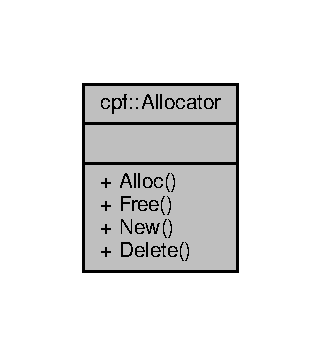
\includegraphics[width=154pt]{classcpf_1_1_allocator__coll__graph}
\end{center}
\end{figure}
\subsection*{정적 Public 멤버 함수}
\begin{DoxyCompactItemize}
\item 
{\footnotesize template$<$typename T $>$ }\\static T $\ast$ \hyperlink{classcpf_1_1_allocator_a3481cae5807aa57faf8ac9157bd5c618}{Alloc} (uint32\+\_\+t num=1)
\item 
{\footnotesize template$<$typename T $>$ }\\static void \hyperlink{classcpf_1_1_allocator_af63eadbfa53045d7eede980fd5d15eb4}{Free} (T $\ast$ptr)
\item 
{\footnotesize template$<$typename T , class ... Args$>$ }\\static T $\ast$ \hyperlink{classcpf_1_1_allocator_ab224979f67fae21e9db39b211a67b2e9}{New} (Args \&\&... args)
\item 
{\footnotesize template$<$typename T $>$ }\\static void \hyperlink{classcpf_1_1_allocator_a6c7808c532c47dc997deaf296aae4f27}{Delete} (T $\ast$ptr)
\end{DoxyCompactItemize}


\subsection{상세한 설명}
메모리 할당을 도와줄 핼퍼 클래스입니다. 

System.\+hpp 파일의 7 번째 라인에서 정의되었습니다.



\subsection{멤버 함수 문서화}
\mbox{\Hypertarget{classcpf_1_1_allocator_a3481cae5807aa57faf8ac9157bd5c618}\label{classcpf_1_1_allocator_a3481cae5807aa57faf8ac9157bd5c618}} 
\index{cpf\+::\+Allocator@{cpf\+::\+Allocator}!Alloc@{Alloc}}
\index{Alloc@{Alloc}!cpf\+::\+Allocator@{cpf\+::\+Allocator}}
\subsubsection{\texorpdfstring{Alloc()}{Alloc()}}
{\footnotesize\ttfamily template$<$typename T $>$ \\
static T$\ast$ cpf\+::\+Allocator\+::\+Alloc (\begin{DoxyParamCaption}\item[{uint32\+\_\+t}]{num = {\ttfamily 1} }\end{DoxyParamCaption})\hspace{0.3cm}{\ttfamily [inline]}, {\ttfamily [static]}}

주어진 타입을 num만큼 생성합니다. 
\begin{DoxyTemplParams}{Template Parameters}
{\em T} & 생성할 타입. \\
\hline
\end{DoxyTemplParams}

\begin{DoxyParams}{매개변수}
{\em num} & 생성할 수량. 기본 값은 1입니다. \\
\hline
\end{DoxyParams}


System.\+hpp 파일의 15 번째 라인에서 정의되었습니다.


\begin{DoxyCode}
15                                           \{
16             \textcolor{keywordflow}{return} \textcolor{keyword}{static\_cast<}T *\textcolor{keyword}{>}(malloc(\textcolor{keyword}{sizeof}(T) * num));
17         \}
\end{DoxyCode}
\mbox{\Hypertarget{classcpf_1_1_allocator_a6c7808c532c47dc997deaf296aae4f27}\label{classcpf_1_1_allocator_a6c7808c532c47dc997deaf296aae4f27}} 
\index{cpf\+::\+Allocator@{cpf\+::\+Allocator}!Delete@{Delete}}
\index{Delete@{Delete}!cpf\+::\+Allocator@{cpf\+::\+Allocator}}
\subsubsection{\texorpdfstring{Delete()}{Delete()}}
{\footnotesize\ttfamily template$<$typename T $>$ \\
static void cpf\+::\+Allocator\+::\+Delete (\begin{DoxyParamCaption}\item[{T $\ast$}]{ptr }\end{DoxyParamCaption})\hspace{0.3cm}{\ttfamily [inline]}, {\ttfamily [static]}}

주어진 객체를 파괴자 호출 후 해제합니다. 

System.\+hpp 파일의 39 번째 라인에서 정의되었습니다.


\begin{DoxyCode}
39                                    \{
40             ptr->~T();
41             \hyperlink{classcpf_1_1_allocator_af63eadbfa53045d7eede980fd5d15eb4}{Free}(ptr);
42         \}
\end{DoxyCode}
\mbox{\Hypertarget{classcpf_1_1_allocator_af63eadbfa53045d7eede980fd5d15eb4}\label{classcpf_1_1_allocator_af63eadbfa53045d7eede980fd5d15eb4}} 
\index{cpf\+::\+Allocator@{cpf\+::\+Allocator}!Free@{Free}}
\index{Free@{Free}!cpf\+::\+Allocator@{cpf\+::\+Allocator}}
\subsubsection{\texorpdfstring{Free()}{Free()}}
{\footnotesize\ttfamily template$<$typename T $>$ \\
static void cpf\+::\+Allocator\+::\+Free (\begin{DoxyParamCaption}\item[{T $\ast$}]{ptr }\end{DoxyParamCaption})\hspace{0.3cm}{\ttfamily [inline]}, {\ttfamily [static]}}

주어진 객체를 해제시킵니다. 

System.\+hpp 파일의 23 번째 라인에서 정의되었습니다.


\begin{DoxyCode}
23                                  \{
24             free(ptr);
25         \}
\end{DoxyCode}
\mbox{\Hypertarget{classcpf_1_1_allocator_ab224979f67fae21e9db39b211a67b2e9}\label{classcpf_1_1_allocator_ab224979f67fae21e9db39b211a67b2e9}} 
\index{cpf\+::\+Allocator@{cpf\+::\+Allocator}!New@{New}}
\index{New@{New}!cpf\+::\+Allocator@{cpf\+::\+Allocator}}
\subsubsection{\texorpdfstring{New()}{New()}}
{\footnotesize\ttfamily template$<$typename T , class ... Args$>$ \\
static T$\ast$ cpf\+::\+Allocator\+::\+New (\begin{DoxyParamCaption}\item[{Args \&\&...}]{args }\end{DoxyParamCaption})\hspace{0.3cm}{\ttfamily [inline]}, {\ttfamily [static]}}

주어진 타입을 인자로 생성합니다. 

System.\+hpp 파일의 31 번째 라인에서 정의되었습니다.


\begin{DoxyCode}
31                                        \{
32             \textcolor{keywordflow}{return} \textcolor{keyword}{new} (Alloc<T>()) T(std::forward<Args>(args)...);
33         \}
\end{DoxyCode}


이 클래스에 대한 문서화 페이지는 다음의 파일로부터 생성되었습니다.\+:\begin{DoxyCompactItemize}
\item 
Source/\+Foundation/\+Alloc/\hyperlink{_system_8hpp}{System.\+hpp}\end{DoxyCompactItemize}

\hypertarget{classcpf_1_1_application}{}\section{cpf\+:\+:Application 클래스 참조}
\label{classcpf_1_1_application}\index{cpf\+::\+Application@{cpf\+::\+Application}}


{\ttfamily \#include $<$Application.\+hpp$>$}



cpf\+:\+:Application에 대한 상속 다이어그램 \+: 
\nopagebreak
\begin{figure}[H]
\begin{center}
\leavevmode
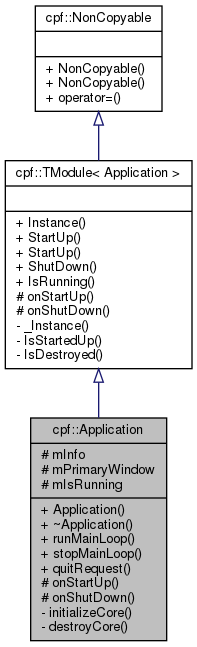
\includegraphics[height=550pt]{classcpf_1_1_application__inherit__graph}
\end{center}
\end{figure}


cpf\+:\+:Application에 대한 협력 다이어그램\+:
\nopagebreak
\begin{figure}[H]
\begin{center}
\leavevmode
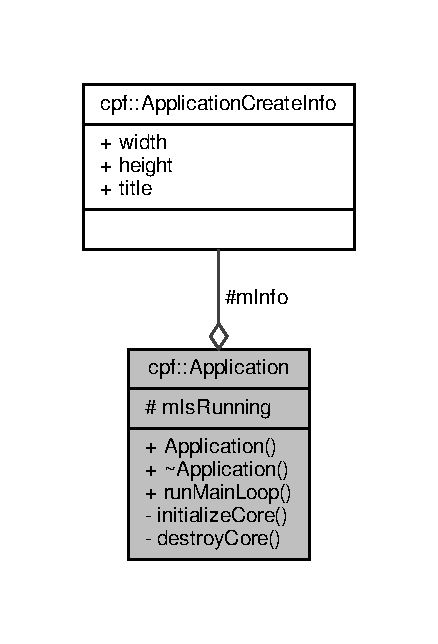
\includegraphics[width=350pt]{classcpf_1_1_application__coll__graph}
\end{center}
\end{figure}
\subsection*{Public 멤버 함수}
\begin{DoxyCompactItemize}
\item 
\hyperlink{classcpf_1_1_application_a82aea6d89660d4ae9898a437f96d2e42}{Application} (const \hyperlink{structcpf_1_1_application_create_info}{Application\+Create\+Info} \&info)
\item 
virtual \hyperlink{classcpf_1_1_application_ad018a98c533cbf877ae11a05b329c4a2}{$\sim$\+Application} ()
\item 
void \hyperlink{classcpf_1_1_application_a52e76d84434e072ad6dafdf7a0f4fd59}{run\+Main\+Loop} ()
\item 
void \hyperlink{classcpf_1_1_application_a527bcad0b3cf7a33ccc8de9318c6d984}{stop\+Main\+Loop} ()
\item 
void \hyperlink{classcpf_1_1_application_ac5c5b81ebccee1f09d777a9fc200eca6}{quit\+Request} ()
\end{DoxyCompactItemize}
\subsection*{정적 Public 멤버 함수}
\begin{DoxyCompactItemize}
\item 
static \hyperlink{classcpf_1_1_application}{Application} \& \hyperlink{classcpf_1_1_t_module_ac8065254584cb0a6656c42f96859d190}{Instance} ()
\item 
static void \hyperlink{classcpf_1_1_t_module_a02fbf3c4d28a3328e81b0e8d0bdd93b0}{Start\+Up} (Args \&\&...args)
\item 
static void \hyperlink{classcpf_1_1_t_module_ac553266ad6255da045ef3f34b0f9bc16}{Start\+Up} (Args \&\&...args)
\item 
static void \hyperlink{classcpf_1_1_t_module_a61452801c61e2546b75a7a6a545e82ee}{Shut\+Down} ()
\item 
static bool \hyperlink{classcpf_1_1_t_module_acd38943803d522ba6dcf7f0871b2f502}{Is\+Running} ()
\end{DoxyCompactItemize}
\subsection*{Protected 멤버 함수}
\begin{DoxyCompactItemize}
\item 
void \hyperlink{classcpf_1_1_application_ae8e759c8722c48c45dc3e02446062aec}{on\+Start\+Up} () override
\item 
void \hyperlink{classcpf_1_1_application_afa25d5eb462d3d5b1ce19c6d217fe9e7}{on\+Shut\+Down} () override
\end{DoxyCompactItemize}
\subsection*{Protected 속성}
\begin{DoxyCompactItemize}
\item 
\hyperlink{structcpf_1_1_application_create_info}{Application\+Create\+Info} \hyperlink{classcpf_1_1_application_aeef620fe71f2ac891e3650d6d3462b28}{m\+Info}
\item 
\hyperlink{namespacecpf_af5ffcc39bb6465427fc3b91366c917f6}{H\+Render\+Window} \hyperlink{classcpf_1_1_application_a112167287be2ff0ee64a793c6a93fa3d}{m\+Primary\+Window}
\item 
bool \hyperlink{classcpf_1_1_application_a84a6e2bafcc39719acee9885a064ac75}{m\+Is\+Running}
\end{DoxyCompactItemize}
\subsection*{Private 멤버 함수}
\begin{DoxyCompactItemize}
\item 
void \hyperlink{classcpf_1_1_application_a676898244f732414360ced11ed65379c}{initialize\+Core} ()
\item 
void \hyperlink{classcpf_1_1_application_aa65f415f1e0866cab063d83ab428ebbc}{destroy\+Core} ()
\end{DoxyCompactItemize}


\subsection{상세한 설명}
어플리케이션의 메인 모듈입니다. 

Application.\+hpp 파일의 21 번째 라인에서 정의되었습니다.



\subsection{생성자 \& 소멸자 문서화}
\mbox{\Hypertarget{classcpf_1_1_application_a82aea6d89660d4ae9898a437f96d2e42}\label{classcpf_1_1_application_a82aea6d89660d4ae9898a437f96d2e42}} 
\index{cpf\+::\+Application@{cpf\+::\+Application}!Application@{Application}}
\index{Application@{Application}!cpf\+::\+Application@{cpf\+::\+Application}}
\subsubsection{\texorpdfstring{Application()}{Application()}}
{\footnotesize\ttfamily cpf\+::\+Application\+::\+Application (\begin{DoxyParamCaption}\item[{const \hyperlink{structcpf_1_1_application_create_info}{Application\+Create\+Info} \&}]{info }\end{DoxyParamCaption})}



Application.\+cpp 파일의 15 번째 라인에서 정의되었습니다.


\begin{DoxyCode}
15                                                               : \hyperlink{classcpf_1_1_application_aeef620fe71f2ac891e3650d6d3462b28}{mInfo}(info), 
      \hyperlink{classcpf_1_1_application_a84a6e2bafcc39719acee9885a064ac75}{mIsRunning}(\textcolor{keyword}{false}) \{
16     \}
\end{DoxyCode}
\mbox{\Hypertarget{classcpf_1_1_application_ad018a98c533cbf877ae11a05b329c4a2}\label{classcpf_1_1_application_ad018a98c533cbf877ae11a05b329c4a2}} 
\index{cpf\+::\+Application@{cpf\+::\+Application}!````~Application@{$\sim$\+Application}}
\index{````~Application@{$\sim$\+Application}!cpf\+::\+Application@{cpf\+::\+Application}}
\subsubsection{\texorpdfstring{$\sim$\+Application()}{~Application()}}
{\footnotesize\ttfamily cpf\+::\+Application\+::$\sim$\+Application (\begin{DoxyParamCaption}{ }\end{DoxyParamCaption})\hspace{0.3cm}{\ttfamily [virtual]}}



Application.\+cpp 파일의 18 번째 라인에서 정의되었습니다.


\begin{DoxyCode}
18                               \{
19     \}
\end{DoxyCode}


\subsection{멤버 함수 문서화}
\mbox{\Hypertarget{classcpf_1_1_application_aa65f415f1e0866cab063d83ab428ebbc}\label{classcpf_1_1_application_aa65f415f1e0866cab063d83ab428ebbc}} 
\index{cpf\+::\+Application@{cpf\+::\+Application}!destroy\+Core@{destroy\+Core}}
\index{destroy\+Core@{destroy\+Core}!cpf\+::\+Application@{cpf\+::\+Application}}
\subsubsection{\texorpdfstring{destroy\+Core()}{destroyCore()}}
{\footnotesize\ttfamily void cpf\+::\+Application\+::destroy\+Core (\begin{DoxyParamCaption}{ }\end{DoxyParamCaption})\hspace{0.3cm}{\ttfamily [private]}}



Application.\+cpp 파일의 56 번째 라인에서 정의되었습니다.


\begin{DoxyCode}
56                                   \{
57         \hyperlink{classcpf_1_1_t_module_a61452801c61e2546b75a7a6a545e82ee}{RenderWindowManager::ShutDown}();
58 
59         glfwTerminate();
60     \}
\end{DoxyCode}
\mbox{\Hypertarget{classcpf_1_1_application_a676898244f732414360ced11ed65379c}\label{classcpf_1_1_application_a676898244f732414360ced11ed65379c}} 
\index{cpf\+::\+Application@{cpf\+::\+Application}!initialize\+Core@{initialize\+Core}}
\index{initialize\+Core@{initialize\+Core}!cpf\+::\+Application@{cpf\+::\+Application}}
\subsubsection{\texorpdfstring{initialize\+Core()}{initializeCore()}}
{\footnotesize\ttfamily void cpf\+::\+Application\+::initialize\+Core (\begin{DoxyParamCaption}{ }\end{DoxyParamCaption})\hspace{0.3cm}{\ttfamily [private]}}



Application.\+cpp 파일의 45 번째 라인에서 정의되었습니다.


\begin{DoxyCode}
45                                      \{
46         \textcolor{keywordflow}{if} (!glfwInit()) \{
47             \hyperlink{classcpf_1_1_debug_a22849847c74bcb444922c263c9ae6183}{Debug::LogFatal}(\textcolor{stringliteral}{"Failed to initialize glfw!"});
48         \}
49 
50         glfwSetErrorCallback(\hyperlink{namespacecpf_a2aa8b9856909234833858da9b6c466dd}{glfwErrorCallback});
51         \hyperlink{classcpf_1_1_t_module_a02fbf3c4d28a3328e81b0e8d0bdd93b0}{RenderWindowManager::StartUp}();
52 
53         \hyperlink{classcpf_1_1_application_a112167287be2ff0ee64a793c6a93fa3d}{mPrimaryWindow} = \hyperlink{classcpf_1_1_t_module_ac8065254584cb0a6656c42f96859d190}{RenderWindowManager::Instance}().
      \hyperlink{classcpf_1_1_render_window_manager_a9e198c25b9f2eb5dd5b248e47532677d}{initialize}(\hyperlink{classcpf_1_1_application_aeef620fe71f2ac891e3650d6d3462b28}{mInfo}.\hyperlink{structcpf_1_1_application_create_info_a1cd605f921ac5ac29474cbe52f7ea499}{primaryWindowCreateInfo});
54     \}
\end{DoxyCode}
\mbox{\Hypertarget{classcpf_1_1_t_module_ac8065254584cb0a6656c42f96859d190}\label{classcpf_1_1_t_module_ac8065254584cb0a6656c42f96859d190}} 
\index{cpf\+::\+Application@{cpf\+::\+Application}!Instance@{Instance}}
\index{Instance@{Instance}!cpf\+::\+Application@{cpf\+::\+Application}}
\subsubsection{\texorpdfstring{Instance()}{Instance()}}
{\footnotesize\ttfamily static \hyperlink{classcpf_1_1_application}{Application} \& \hyperlink{classcpf_1_1_t_module}{cpf\+::\+T\+Module}$<$ \hyperlink{classcpf_1_1_application}{Application}  $>$\+::Instance (\begin{DoxyParamCaption}{ }\end{DoxyParamCaption})\hspace{0.3cm}{\ttfamily [inline]}, {\ttfamily [static]}, {\ttfamily [inherited]}}

모듈 객체의 참조를 반환합니다. \begin{DoxyWarning}{경고}
모듈이 실행중이 아니라면 에러를 출력하고 프로그램이 종료됩니다. 
\end{DoxyWarning}


Module.\+hpp 파일의 32 번째 라인에서 정의되었습니다.


\begin{DoxyCode}
32                              \{
33             \textcolor{keywordflow}{if} (!\hyperlink{classcpf_1_1_t_module_a73732afee7131dad652bf3e00c75cef9}{IsStartedUp}()) \{
34                 Debug::LogFatal(\textcolor{stringliteral}{"Trying to access not start module!"});
35             \}
36 
37             \textcolor{keywordflow}{if} (\hyperlink{classcpf_1_1_t_module_a9f70f0a70ac59b13b7a874f82c877337}{IsDestroyed}()) \{
38                 Debug::LogFatal(\textcolor{stringliteral}{"Trying to access destroyed module!"});
39             \}
40 
41             \textcolor{keywordflow}{return} *\hyperlink{classcpf_1_1_t_module_a06ab8af8ea6b294959937fd2bbc1e615}{\_Instance}();
42         \}
\end{DoxyCode}
\mbox{\Hypertarget{classcpf_1_1_t_module_acd38943803d522ba6dcf7f0871b2f502}\label{classcpf_1_1_t_module_acd38943803d522ba6dcf7f0871b2f502}} 
\index{cpf\+::\+Application@{cpf\+::\+Application}!Is\+Running@{Is\+Running}}
\index{Is\+Running@{Is\+Running}!cpf\+::\+Application@{cpf\+::\+Application}}
\subsubsection{\texorpdfstring{Is\+Running()}{IsRunning()}}
{\footnotesize\ttfamily static bool \hyperlink{classcpf_1_1_t_module}{cpf\+::\+T\+Module}$<$ \hyperlink{classcpf_1_1_application}{Application}  $>$\+::Is\+Running (\begin{DoxyParamCaption}{ }\end{DoxyParamCaption})\hspace{0.3cm}{\ttfamily [inline]}, {\ttfamily [static]}, {\ttfamily [inherited]}}

모듈이 실행 중인지 확인합니다. 

Module.\+hpp 파일의 108 번째 라인에서 정의되었습니다.


\begin{DoxyCode}
108                                 \{
109             \textcolor{keywordflow}{return} \hyperlink{classcpf_1_1_t_module_a73732afee7131dad652bf3e00c75cef9}{IsStartedUp}() && !\hyperlink{classcpf_1_1_t_module_a9f70f0a70ac59b13b7a874f82c877337}{IsDestroyed}();
110         \}
\end{DoxyCode}
\mbox{\Hypertarget{classcpf_1_1_application_afa25d5eb462d3d5b1ce19c6d217fe9e7}\label{classcpf_1_1_application_afa25d5eb462d3d5b1ce19c6d217fe9e7}} 
\index{cpf\+::\+Application@{cpf\+::\+Application}!on\+Shut\+Down@{on\+Shut\+Down}}
\index{on\+Shut\+Down@{on\+Shut\+Down}!cpf\+::\+Application@{cpf\+::\+Application}}
\subsubsection{\texorpdfstring{on\+Shut\+Down()}{onShutDown()}}
{\footnotesize\ttfamily void cpf\+::\+Application\+::on\+Shut\+Down (\begin{DoxyParamCaption}{ }\end{DoxyParamCaption})\hspace{0.3cm}{\ttfamily [override]}, {\ttfamily [protected]}, {\ttfamily [virtual]}}

모듈 해제 직전에 호출됩니다. \begin{DoxyNote}{주의}
해제 직전에 처리해야할 문제가 있다면 해당 함수를 재정의 하세요. 
\end{DoxyNote}


\hyperlink{classcpf_1_1_t_module_a15c93b1aca54022e145961bea8e3ea7d}{cpf\+::\+T\+Module$<$ Application $>$}(으)로부터 재구현되었습니다.



Application.\+cpp 파일의 41 번째 라인에서 정의되었습니다.


\begin{DoxyCode}
41                                  \{
42         \hyperlink{classcpf_1_1_application_aa65f415f1e0866cab063d83ab428ebbc}{destroyCore}();
43     \}
\end{DoxyCode}
\mbox{\Hypertarget{classcpf_1_1_application_ae8e759c8722c48c45dc3e02446062aec}\label{classcpf_1_1_application_ae8e759c8722c48c45dc3e02446062aec}} 
\index{cpf\+::\+Application@{cpf\+::\+Application}!on\+Start\+Up@{on\+Start\+Up}}
\index{on\+Start\+Up@{on\+Start\+Up}!cpf\+::\+Application@{cpf\+::\+Application}}
\subsubsection{\texorpdfstring{on\+Start\+Up()}{onStartUp()}}
{\footnotesize\ttfamily void cpf\+::\+Application\+::on\+Start\+Up (\begin{DoxyParamCaption}{ }\end{DoxyParamCaption})\hspace{0.3cm}{\ttfamily [override]}, {\ttfamily [protected]}, {\ttfamily [virtual]}}

모듈 생성 직후에 호출됩니다. \begin{DoxyNote}{주의}
할당 직후에 처리해야할 문제가 있다면 해당 함수를 재정의 하세요. 
\end{DoxyNote}


\hyperlink{classcpf_1_1_t_module_a4eb83b0848794e422d2d345439f51a04}{cpf\+::\+T\+Module$<$ Application $>$}(으)로부터 재구현되었습니다.



Application.\+cpp 파일의 37 번째 라인에서 정의되었습니다.


\begin{DoxyCode}
37                                 \{
38         \hyperlink{classcpf_1_1_application_a676898244f732414360ced11ed65379c}{initializeCore}();
39     \}
\end{DoxyCode}
\mbox{\Hypertarget{classcpf_1_1_application_ac5c5b81ebccee1f09d777a9fc200eca6}\label{classcpf_1_1_application_ac5c5b81ebccee1f09d777a9fc200eca6}} 
\index{cpf\+::\+Application@{cpf\+::\+Application}!quit\+Request@{quit\+Request}}
\index{quit\+Request@{quit\+Request}!cpf\+::\+Application@{cpf\+::\+Application}}
\subsubsection{\texorpdfstring{quit\+Request()}{quitRequest()}}
{\footnotesize\ttfamily void cpf\+::\+Application\+::quit\+Request (\begin{DoxyParamCaption}{ }\end{DoxyParamCaption})}



Application.\+cpp 파일의 33 번째 라인에서 정의되었습니다.


\begin{DoxyCode}
33                                   \{
34         \hyperlink{classcpf_1_1_application_a527bcad0b3cf7a33ccc8de9318c6d984}{stopMainLoop}();
35     \}
\end{DoxyCode}
\mbox{\Hypertarget{classcpf_1_1_application_a52e76d84434e072ad6dafdf7a0f4fd59}\label{classcpf_1_1_application_a52e76d84434e072ad6dafdf7a0f4fd59}} 
\index{cpf\+::\+Application@{cpf\+::\+Application}!run\+Main\+Loop@{run\+Main\+Loop}}
\index{run\+Main\+Loop@{run\+Main\+Loop}!cpf\+::\+Application@{cpf\+::\+Application}}
\subsubsection{\texorpdfstring{run\+Main\+Loop()}{runMainLoop()}}
{\footnotesize\ttfamily void cpf\+::\+Application\+::run\+Main\+Loop (\begin{DoxyParamCaption}{ }\end{DoxyParamCaption})}



Application.\+cpp 파일의 21 번째 라인에서 정의되었습니다.


\begin{DoxyCode}
21                                   \{
22         \hyperlink{classcpf_1_1_application_a84a6e2bafcc39719acee9885a064ac75}{mIsRunning} = \textcolor{keyword}{true};
23 
24         \textcolor{keywordflow}{while} (\hyperlink{classcpf_1_1_application_a84a6e2bafcc39719acee9885a064ac75}{mIsRunning}) \{
25             \hyperlink{classcpf_1_1_t_module_ac8065254584cb0a6656c42f96859d190}{RenderWindowManager::Instance}().\hyperlink{classcpf_1_1_render_window_manager_adc7ef3bd3f5c4ad9b86899adeb69b0ee}{update}();
26         \}
27     \}
\end{DoxyCode}
\mbox{\Hypertarget{classcpf_1_1_t_module_a61452801c61e2546b75a7a6a545e82ee}\label{classcpf_1_1_t_module_a61452801c61e2546b75a7a6a545e82ee}} 
\index{cpf\+::\+Application@{cpf\+::\+Application}!Shut\+Down@{Shut\+Down}}
\index{Shut\+Down@{Shut\+Down}!cpf\+::\+Application@{cpf\+::\+Application}}
\subsubsection{\texorpdfstring{Shut\+Down()}{ShutDown()}}
{\footnotesize\ttfamily static void \hyperlink{classcpf_1_1_t_module}{cpf\+::\+T\+Module}$<$ \hyperlink{classcpf_1_1_application}{Application}  $>$\+::Shut\+Down (\begin{DoxyParamCaption}{ }\end{DoxyParamCaption})\hspace{0.3cm}{\ttfamily [inline]}, {\ttfamily [static]}, {\ttfamily [inherited]}}

모듈을 종료합니다. \begin{DoxyWarning}{경고}
모듈이 실행 중이 아니라면 에러를 출력하고 프로그램이 종료됩니다. 
\end{DoxyWarning}


Module.\+hpp 파일의 89 번째 라인에서 정의되었습니다.


\begin{DoxyCode}
89                                \{
90             \textcolor{keywordflow}{if} (!\hyperlink{classcpf_1_1_t_module_a73732afee7131dad652bf3e00c75cef9}{IsStartedUp}()) \{
91                 Debug::LogFatal(\textcolor{stringliteral}{"Trying to shut down module start yet"});
92             \}
93 
94             \textcolor{keywordflow}{if} (\hyperlink{classcpf_1_1_t_module_a9f70f0a70ac59b13b7a874f82c877337}{IsDestroyed}()) \{
95                 Debug::LogFatal(\textcolor{stringliteral}{"Trying to shut down module already shut down"});
96             \}
97 
98             \textcolor{keyword}{static\_cast<}TModule<T> *\textcolor{keyword}{>}(\hyperlink{classcpf_1_1_t_module_a06ab8af8ea6b294959937fd2bbc1e615}{\_Instance}())->\hyperlink{classcpf_1_1_t_module_a15c93b1aca54022e145961bea8e3ea7d}{onShutDown}();
99             Allocator::Free(\hyperlink{classcpf_1_1_t_module_a06ab8af8ea6b294959937fd2bbc1e615}{\_Instance}());
100 
101             \hyperlink{classcpf_1_1_t_module_a06ab8af8ea6b294959937fd2bbc1e615}{\_Instance}() = \textcolor{keyword}{nullptr};
102             \hyperlink{classcpf_1_1_t_module_a9f70f0a70ac59b13b7a874f82c877337}{IsDestroyed}() = \textcolor{keyword}{true};
103         \}
\end{DoxyCode}
\mbox{\Hypertarget{classcpf_1_1_t_module_a02fbf3c4d28a3328e81b0e8d0bdd93b0}\label{classcpf_1_1_t_module_a02fbf3c4d28a3328e81b0e8d0bdd93b0}} 
\index{cpf\+::\+Application@{cpf\+::\+Application}!Start\+Up@{Start\+Up}}
\index{Start\+Up@{Start\+Up}!cpf\+::\+Application@{cpf\+::\+Application}}
\subsubsection{\texorpdfstring{Start\+Up()}{StartUp()}\hspace{0.1cm}{\footnotesize\ttfamily [1/2]}}
{\footnotesize\ttfamily static void \hyperlink{classcpf_1_1_t_module}{cpf\+::\+T\+Module}$<$ \hyperlink{classcpf_1_1_application}{Application}  $>$\+::Start\+Up (\begin{DoxyParamCaption}\item[{Args \&\&...}]{args }\end{DoxyParamCaption})\hspace{0.3cm}{\ttfamily [inline]}, {\ttfamily [static]}, {\ttfamily [inherited]}}

모듈을 주어진 인자와 함께 생성합니다. \begin{DoxyWarning}{경고}
모듈이 실행 중이 아니라면 에러를 출력하고 프로그램이 종료됩니다. 
\end{DoxyWarning}


Module.\+hpp 파일의 50 번째 라인에서 정의되었습니다.


\begin{DoxyCode}
50                                             \{
51             \textcolor{keywordflow}{if} (\hyperlink{classcpf_1_1_t_module_a73732afee7131dad652bf3e00c75cef9}{IsStartedUp}()) \{
52                 Debug::LogFatal(\textcolor{stringliteral}{"Trying to start up module already started"});
53             \}
54 
55             \textcolor{keywordflow}{if} (\hyperlink{classcpf_1_1_t_module_a9f70f0a70ac59b13b7a874f82c877337}{IsDestroyed}()) \{
56                 Debug::LogFatal(\textcolor{stringliteral}{"Trying to start up module already destroyed"});
57             \}
58 
59             \hyperlink{classcpf_1_1_t_module_a06ab8af8ea6b294959937fd2bbc1e615}{\_Instance}() = Allocator::New<T>(std::forward<Args>(args)...);
60             \textcolor{keyword}{static\_cast<}TModule<T> *\textcolor{keyword}{>}(\hyperlink{classcpf_1_1_t_module_a06ab8af8ea6b294959937fd2bbc1e615}{\_Instance}())->\hyperlink{classcpf_1_1_t_module_a4eb83b0848794e422d2d345439f51a04}{onStartUp}();
61 
62             \hyperlink{classcpf_1_1_t_module_a73732afee7131dad652bf3e00c75cef9}{IsStartedUp}() = \textcolor{keyword}{true};
63         \}
\end{DoxyCode}
\mbox{\Hypertarget{classcpf_1_1_t_module_ac553266ad6255da045ef3f34b0f9bc16}\label{classcpf_1_1_t_module_ac553266ad6255da045ef3f34b0f9bc16}} 
\index{cpf\+::\+Application@{cpf\+::\+Application}!Start\+Up@{Start\+Up}}
\index{Start\+Up@{Start\+Up}!cpf\+::\+Application@{cpf\+::\+Application}}
\subsubsection{\texorpdfstring{Start\+Up()}{StartUp()}\hspace{0.1cm}{\footnotesize\ttfamily [2/2]}}
{\footnotesize\ttfamily static void \hyperlink{classcpf_1_1_t_module}{cpf\+::\+T\+Module}$<$ \hyperlink{classcpf_1_1_application}{Application}  $>$\+::Start\+Up (\begin{DoxyParamCaption}\item[{Args \&\&...}]{args }\end{DoxyParamCaption})\hspace{0.3cm}{\ttfamily [inline]}, {\ttfamily [static]}, {\ttfamily [inherited]}}

모듈을 주어진 하위 시스템과 인자로 생성합니다. \begin{DoxyWarning}{경고}
모듈이 실행 중이 아니라면 에러를 출력하고 프로그램이 종료됩니다. 
\end{DoxyWarning}


Module.\+hpp 파일의 70 번째 라인에서 정의되었습니다.


\begin{DoxyCode}
70                                             \{
71             \textcolor{keywordflow}{if} (\hyperlink{classcpf_1_1_t_module_a73732afee7131dad652bf3e00c75cef9}{IsStartedUp}()) \{
72                 Debug::LogFatal(\textcolor{stringliteral}{"Trying to start up module already started"});
73             \}
74 
75             \textcolor{keywordflow}{if} (\hyperlink{classcpf_1_1_t_module_a9f70f0a70ac59b13b7a874f82c877337}{IsDestroyed}()) \{
76                 Debug::LogFatal(\textcolor{stringliteral}{"Trying to start up module already destroyed"});
77             \}
78 
79             \hyperlink{classcpf_1_1_t_module_a06ab8af8ea6b294959937fd2bbc1e615}{\_Instance}() = Allocator::New<U>(std::forward<Args>(args)...);
80             \textcolor{keyword}{static\_cast<}TModule<T> *\textcolor{keyword}{>}(\hyperlink{classcpf_1_1_t_module_a06ab8af8ea6b294959937fd2bbc1e615}{\_Instance}())->\hyperlink{classcpf_1_1_t_module_a15c93b1aca54022e145961bea8e3ea7d}{onShutDown}();
81 
82             \hyperlink{classcpf_1_1_t_module_a73732afee7131dad652bf3e00c75cef9}{IsStartedUp}() = \textcolor{keyword}{true};
83         \}
\end{DoxyCode}
\mbox{\Hypertarget{classcpf_1_1_application_a527bcad0b3cf7a33ccc8de9318c6d984}\label{classcpf_1_1_application_a527bcad0b3cf7a33ccc8de9318c6d984}} 
\index{cpf\+::\+Application@{cpf\+::\+Application}!stop\+Main\+Loop@{stop\+Main\+Loop}}
\index{stop\+Main\+Loop@{stop\+Main\+Loop}!cpf\+::\+Application@{cpf\+::\+Application}}
\subsubsection{\texorpdfstring{stop\+Main\+Loop()}{stopMainLoop()}}
{\footnotesize\ttfamily void cpf\+::\+Application\+::stop\+Main\+Loop (\begin{DoxyParamCaption}{ }\end{DoxyParamCaption})}



Application.\+cpp 파일의 29 번째 라인에서 정의되었습니다.


\begin{DoxyCode}
29                                    \{
30         \hyperlink{classcpf_1_1_application_a84a6e2bafcc39719acee9885a064ac75}{mIsRunning} = \textcolor{keyword}{false};
31     \}
\end{DoxyCode}


\subsection{멤버 데이터 문서화}
\mbox{\Hypertarget{classcpf_1_1_application_aeef620fe71f2ac891e3650d6d3462b28}\label{classcpf_1_1_application_aeef620fe71f2ac891e3650d6d3462b28}} 
\index{cpf\+::\+Application@{cpf\+::\+Application}!m\+Info@{m\+Info}}
\index{m\+Info@{m\+Info}!cpf\+::\+Application@{cpf\+::\+Application}}
\subsubsection{\texorpdfstring{m\+Info}{mInfo}}
{\footnotesize\ttfamily \hyperlink{structcpf_1_1_application_create_info}{Application\+Create\+Info} cpf\+::\+Application\+::m\+Info\hspace{0.3cm}{\ttfamily [protected]}}



Application.\+hpp 파일의 23 번째 라인에서 정의되었습니다.

\mbox{\Hypertarget{classcpf_1_1_application_a84a6e2bafcc39719acee9885a064ac75}\label{classcpf_1_1_application_a84a6e2bafcc39719acee9885a064ac75}} 
\index{cpf\+::\+Application@{cpf\+::\+Application}!m\+Is\+Running@{m\+Is\+Running}}
\index{m\+Is\+Running@{m\+Is\+Running}!cpf\+::\+Application@{cpf\+::\+Application}}
\subsubsection{\texorpdfstring{m\+Is\+Running}{mIsRunning}}
{\footnotesize\ttfamily bool cpf\+::\+Application\+::m\+Is\+Running\hspace{0.3cm}{\ttfamily [protected]}}



Application.\+hpp 파일의 26 번째 라인에서 정의되었습니다.

\mbox{\Hypertarget{classcpf_1_1_application_a112167287be2ff0ee64a793c6a93fa3d}\label{classcpf_1_1_application_a112167287be2ff0ee64a793c6a93fa3d}} 
\index{cpf\+::\+Application@{cpf\+::\+Application}!m\+Primary\+Window@{m\+Primary\+Window}}
\index{m\+Primary\+Window@{m\+Primary\+Window}!cpf\+::\+Application@{cpf\+::\+Application}}
\subsubsection{\texorpdfstring{m\+Primary\+Window}{mPrimaryWindow}}
{\footnotesize\ttfamily \hyperlink{namespacecpf_af5ffcc39bb6465427fc3b91366c917f6}{H\+Render\+Window} cpf\+::\+Application\+::m\+Primary\+Window\hspace{0.3cm}{\ttfamily [protected]}}



Application.\+hpp 파일의 25 번째 라인에서 정의되었습니다.



이 클래스에 대한 문서화 페이지는 다음의 파일들로부터 생성되었습니다.\+:\begin{DoxyCompactItemize}
\item 
Source/\+Foundation/\hyperlink{_application_8hpp}{Application.\+hpp}\item 
Source/\+Foundation/\hyperlink{_application_8cpp}{Application.\+cpp}\end{DoxyCompactItemize}

\hypertarget{structcpf_1_1_application_create_info}{}\section{cpf\+:\+:Application\+Create\+Info 구조체 참조}
\label{structcpf_1_1_application_create_info}\index{cpf\+::\+Application\+Create\+Info@{cpf\+::\+Application\+Create\+Info}}


{\ttfamily \#include $<$Application.\+hpp$>$}



cpf\+:\+:Application\+Create\+Info에 대한 협력 다이어그램\+:\nopagebreak
\begin{figure}[H]
\begin{center}
\leavevmode
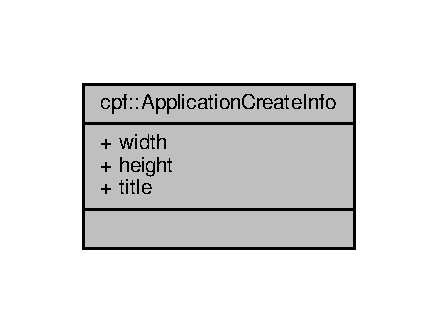
\includegraphics[width=210pt]{structcpf_1_1_application_create_info__coll__graph}
\end{center}
\end{figure}
\subsection*{Public 속성}
\begin{DoxyCompactItemize}
\item 
uint32\+\_\+t \hyperlink{structcpf_1_1_application_create_info_a5fbc8d17129dfb2bfe37432132e214c0}{width}
\item 
uint32\+\_\+t \hyperlink{structcpf_1_1_application_create_info_ad4f22ba65d9f55b667fe38a729166ec1}{height}
\item 
\hyperlink{namespacecpf_a4dbd6992c3ed4440ce7ed8982ff7ffea}{String} \hyperlink{structcpf_1_1_application_create_info_a524aeb95e2ea78c56409a0d60f211be2}{title}
\end{DoxyCompactItemize}


\subsection{상세한 설명}


Application.\+hpp 파일의 6 번째 라인에서 정의되었습니다.



\subsection{멤버 데이터 문서화}
\mbox{\Hypertarget{structcpf_1_1_application_create_info_ad4f22ba65d9f55b667fe38a729166ec1}\label{structcpf_1_1_application_create_info_ad4f22ba65d9f55b667fe38a729166ec1}} 
\index{cpf\+::\+Application\+Create\+Info@{cpf\+::\+Application\+Create\+Info}!height@{height}}
\index{height@{height}!cpf\+::\+Application\+Create\+Info@{cpf\+::\+Application\+Create\+Info}}
\subsubsection{\texorpdfstring{height}{height}}
{\footnotesize\ttfamily uint32\+\_\+t cpf\+::\+Application\+Create\+Info\+::height}



Application.\+hpp 파일의 7 번째 라인에서 정의되었습니다.

\mbox{\Hypertarget{structcpf_1_1_application_create_info_a524aeb95e2ea78c56409a0d60f211be2}\label{structcpf_1_1_application_create_info_a524aeb95e2ea78c56409a0d60f211be2}} 
\index{cpf\+::\+Application\+Create\+Info@{cpf\+::\+Application\+Create\+Info}!title@{title}}
\index{title@{title}!cpf\+::\+Application\+Create\+Info@{cpf\+::\+Application\+Create\+Info}}
\subsubsection{\texorpdfstring{title}{title}}
{\footnotesize\ttfamily \hyperlink{namespacecpf_a4dbd6992c3ed4440ce7ed8982ff7ffea}{String} cpf\+::\+Application\+Create\+Info\+::title}



Application.\+hpp 파일의 8 번째 라인에서 정의되었습니다.

\mbox{\Hypertarget{structcpf_1_1_application_create_info_a5fbc8d17129dfb2bfe37432132e214c0}\label{structcpf_1_1_application_create_info_a5fbc8d17129dfb2bfe37432132e214c0}} 
\index{cpf\+::\+Application\+Create\+Info@{cpf\+::\+Application\+Create\+Info}!width@{width}}
\index{width@{width}!cpf\+::\+Application\+Create\+Info@{cpf\+::\+Application\+Create\+Info}}
\subsubsection{\texorpdfstring{width}{width}}
{\footnotesize\ttfamily uint32\+\_\+t cpf\+::\+Application\+Create\+Info\+::width}



Application.\+hpp 파일의 7 번째 라인에서 정의되었습니다.



이 구조체에 대한 문서화 페이지는 다음의 파일로부터 생성되었습니다.\+:\begin{DoxyCompactItemize}
\item 
Source/\+Foundation/\hyperlink{_application_8hpp}{Application.\+hpp}\end{DoxyCompactItemize}

\hypertarget{classcpf_1_1_debug}{}\section{cpf\+:\+:Debug 클래스 참조}
\label{classcpf_1_1_debug}\index{cpf\+::\+Debug@{cpf\+::\+Debug}}


{\ttfamily \#include $<$Debug.\+hpp$>$}



cpf\+:\+:Debug에 대한 협력 다이어그램\+:\nopagebreak
\begin{figure}[H]
\begin{center}
\leavevmode
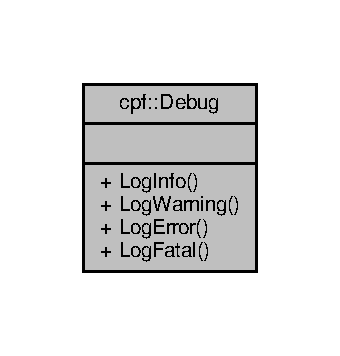
\includegraphics[width=163pt]{classcpf_1_1_debug__coll__graph}
\end{center}
\end{figure}
\subsection*{정적 Public 멤버 함수}
\begin{DoxyCompactItemize}
\item 
{\footnotesize template$<$typename ... Args$>$ }\\static void \hyperlink{classcpf_1_1_debug_a4fdb5fd97498bef70585fcac8047efa2}{Log\+Info} (const \hyperlink{namespacecpf_a4dbd6992c3ed4440ce7ed8982ff7ffea}{String} \&fmt, Args \&\&...args)
\begin{DoxyCompactList}\small\item\em \{\} =$>$ 해당 순서에 맞는 인자를 대입시킵니다. \{n\} =$>$ n에 해당하는 순서에 맞는 인자를 대입시킵니다. \end{DoxyCompactList}\item 
{\footnotesize template$<$typename ... Args$>$ }\\static void \hyperlink{classcpf_1_1_debug_a57373c6a7f52d7d41282596e2eb7d901}{Log\+Warning} (const \hyperlink{namespacecpf_a4dbd6992c3ed4440ce7ed8982ff7ffea}{String} \&fmt, Args \&\&...args)
\item 
{\footnotesize template$<$typename ... Args$>$ }\\static void \hyperlink{classcpf_1_1_debug_a3c867b9c24006a8b45b661b35efea6d2}{Log\+Error} (const \hyperlink{namespacecpf_a4dbd6992c3ed4440ce7ed8982ff7ffea}{String} \&fmt, Args \&\&...args)
\item 
{\footnotesize template$<$typename ... Args$>$ }\\static void \hyperlink{classcpf_1_1_debug_a22849847c74bcb444922c263c9ae6183}{Log\+Fatal} (const \hyperlink{namespacecpf_a4dbd6992c3ed4440ce7ed8982ff7ffea}{String} \&fmt, Args \&\&...args)
\end{DoxyCompactItemize}


\subsection{상세한 설명}
디버깅에 사용할 함수들을 모아놓은 핼퍼 클래스입니다. 

Debug.\+hpp 파일의 9 번째 라인에서 정의되었습니다.



\subsection{멤버 함수 문서화}
\mbox{\Hypertarget{classcpf_1_1_debug_a3c867b9c24006a8b45b661b35efea6d2}\label{classcpf_1_1_debug_a3c867b9c24006a8b45b661b35efea6d2}} 
\index{cpf\+::\+Debug@{cpf\+::\+Debug}!Log\+Error@{Log\+Error}}
\index{Log\+Error@{Log\+Error}!cpf\+::\+Debug@{cpf\+::\+Debug}}
\subsubsection{\texorpdfstring{Log\+Error()}{LogError()}}
{\footnotesize\ttfamily template$<$typename ... Args$>$ \\
static void cpf\+::\+Debug\+::\+Log\+Error (\begin{DoxyParamCaption}\item[{const \hyperlink{namespacecpf_a4dbd6992c3ed4440ce7ed8982ff7ffea}{String} \&}]{fmt,  }\item[{Args \&\&...}]{args }\end{DoxyParamCaption})\hspace{0.3cm}{\ttfamily [inline]}, {\ttfamily [static]}}

비정상적인 상황에 맞닥쳤고 부분적으로 오작동 했을 경우가 높은 상황의 정보를 출력합니다. 

Debug.\+hpp 파일의 32 번째 라인에서 정의되었습니다.


\begin{DoxyCode}
32                                                                \{
33             std::cout << \textcolor{stringliteral}{"ERROR:\(\backslash\)t\(\backslash\)t"} << \hyperlink{classcpf_1_1_string_util_a965cca44ea396f01f2f3c5e3851f1001}{StringUtil::Format}(fmt, std::forward<Args>(args)
      ...) << std::endl;
34         \}
\end{DoxyCode}
\mbox{\Hypertarget{classcpf_1_1_debug_a22849847c74bcb444922c263c9ae6183}\label{classcpf_1_1_debug_a22849847c74bcb444922c263c9ae6183}} 
\index{cpf\+::\+Debug@{cpf\+::\+Debug}!Log\+Fatal@{Log\+Fatal}}
\index{Log\+Fatal@{Log\+Fatal}!cpf\+::\+Debug@{cpf\+::\+Debug}}
\subsubsection{\texorpdfstring{Log\+Fatal()}{LogFatal()}}
{\footnotesize\ttfamily template$<$typename ... Args$>$ \\
static void cpf\+::\+Debug\+::\+Log\+Fatal (\begin{DoxyParamCaption}\item[{const \hyperlink{namespacecpf_a4dbd6992c3ed4440ce7ed8982ff7ffea}{String} \&}]{fmt,  }\item[{Args \&\&...}]{args }\end{DoxyParamCaption})\hspace{0.3cm}{\ttfamily [inline]}, {\ttfamily [static]}}

비정상적인 상황에 맞닥쳤고 복구 불가능한 상황의 정보를 출력합니다. 

Debug.\+hpp 파일의 40 번째 라인에서 정의되었습니다.


\begin{DoxyCode}
40                                                                \{
41             std::cout << \textcolor{stringliteral}{"FATAL:\(\backslash\)t\(\backslash\)t"} << \hyperlink{classcpf_1_1_string_util_a965cca44ea396f01f2f3c5e3851f1001}{StringUtil::Format}(fmt, std::forward<Args>(args)
      ...) << std::endl;
42             exit(EXIT\_FAILURE);
43         \}
\end{DoxyCode}
\mbox{\Hypertarget{classcpf_1_1_debug_a4fdb5fd97498bef70585fcac8047efa2}\label{classcpf_1_1_debug_a4fdb5fd97498bef70585fcac8047efa2}} 
\index{cpf\+::\+Debug@{cpf\+::\+Debug}!Log\+Info@{Log\+Info}}
\index{Log\+Info@{Log\+Info}!cpf\+::\+Debug@{cpf\+::\+Debug}}
\subsubsection{\texorpdfstring{Log\+Info()}{LogInfo()}}
{\footnotesize\ttfamily template$<$typename ... Args$>$ \\
static void cpf\+::\+Debug\+::\+Log\+Info (\begin{DoxyParamCaption}\item[{const \hyperlink{namespacecpf_a4dbd6992c3ed4440ce7ed8982ff7ffea}{String} \&}]{fmt,  }\item[{Args \&\&...}]{args }\end{DoxyParamCaption})\hspace{0.3cm}{\ttfamily [inline]}, {\ttfamily [static]}}



\{\} =$>$ 해당 순서에 맞는 인자를 대입시킵니다. \{n\} =$>$ n에 해당하는 순서에 맞는 인자를 대입시킵니다. 

개발, 운영에 도움을 줄 정보를 출력합니다. 주어진 포멧에 맞게 인자들을 재배치시킵니다. \begin{DoxyRefDesc}{할일}
\item[\hyperlink{todo__todo000001}{할일}]해당 위치에 특정한 타입으로 대입 시킬 수 있는 포멧을 추가할 예정입니다. \end{DoxyRefDesc}


Debug.\+hpp 파일의 16 번째 라인에서 정의되었습니다.


\begin{DoxyCode}
16                                                               \{
17             std::cout << \textcolor{stringliteral}{"INFO:\(\backslash\)t\(\backslash\)t"}  << \hyperlink{classcpf_1_1_string_util_a965cca44ea396f01f2f3c5e3851f1001}{StringUtil::Format}(fmt, std::forward<Args>(args)
      ...) << std::endl;
18         \}
\end{DoxyCode}
\mbox{\Hypertarget{classcpf_1_1_debug_a57373c6a7f52d7d41282596e2eb7d901}\label{classcpf_1_1_debug_a57373c6a7f52d7d41282596e2eb7d901}} 
\index{cpf\+::\+Debug@{cpf\+::\+Debug}!Log\+Warning@{Log\+Warning}}
\index{Log\+Warning@{Log\+Warning}!cpf\+::\+Debug@{cpf\+::\+Debug}}
\subsubsection{\texorpdfstring{Log\+Warning()}{LogWarning()}}
{\footnotesize\ttfamily template$<$typename ... Args$>$ \\
static void cpf\+::\+Debug\+::\+Log\+Warning (\begin{DoxyParamCaption}\item[{const \hyperlink{namespacecpf_a4dbd6992c3ed4440ce7ed8982ff7ffea}{String} \&}]{fmt,  }\item[{Args \&\&...}]{args }\end{DoxyParamCaption})\hspace{0.3cm}{\ttfamily [inline]}, {\ttfamily [static]}}

비정상적인 상황에 맞닥쳤지만 해결할 수 있는 상황의 정보를 출력합니다. 

Debug.\+hpp 파일의 24 번째 라인에서 정의되었습니다.


\begin{DoxyCode}
24                                                                  \{
25             std::cout << \textcolor{stringliteral}{"WARNING:\(\backslash\)t"} << \hyperlink{classcpf_1_1_string_util_a965cca44ea396f01f2f3c5e3851f1001}{StringUtil::Format}(fmt, std::forward<Args>(args)
      ...) << std::endl;
26         \}
\end{DoxyCode}


이 클래스에 대한 문서화 페이지는 다음의 파일로부터 생성되었습니다.\+:\begin{DoxyCompactItemize}
\item 
Source/\+Foundation/\+Debug/\hyperlink{_debug_8hpp}{Debug.\+hpp}\end{DoxyCompactItemize}

\hypertarget{classcpf_1_1_non_copyable}{}\section{cpf\+:\+:Non\+Copyable 클래스 참조}
\label{classcpf_1_1_non_copyable}\index{cpf\+::\+Non\+Copyable@{cpf\+::\+Non\+Copyable}}


{\ttfamily \#include $<$Non\+Copyable.\+hpp$>$}



cpf\+:\+:Non\+Copyable에 대한 상속 다이어그램 \+: \nopagebreak
\begin{figure}[H]
\begin{center}
\leavevmode
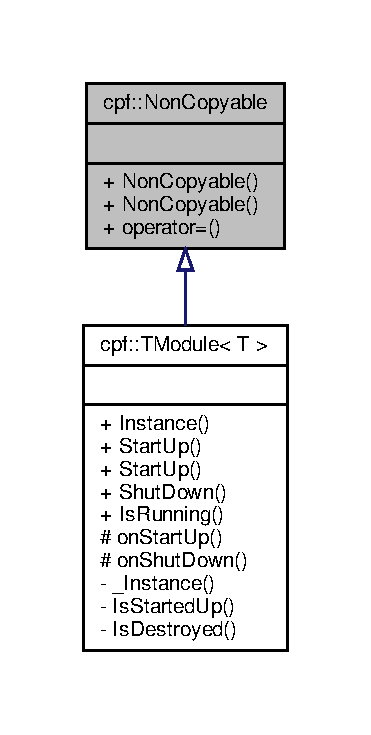
\includegraphics[width=178pt]{classcpf_1_1_non_copyable__inherit__graph}
\end{center}
\end{figure}


cpf\+:\+:Non\+Copyable에 대한 협력 다이어그램\+:\nopagebreak
\begin{figure}[H]
\begin{center}
\leavevmode
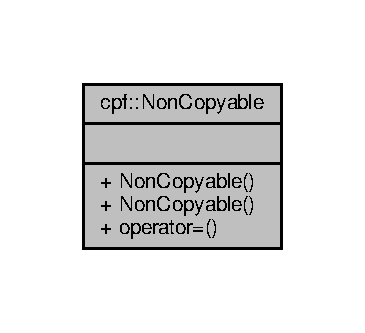
\includegraphics[width=175pt]{classcpf_1_1_non_copyable__coll__graph}
\end{center}
\end{figure}
\subsection*{Public 멤버 함수}
\begin{DoxyCompactItemize}
\item 
\hyperlink{classcpf_1_1_non_copyable_abd233cd8f5e778f7a7ba258e7729092f}{Non\+Copyable} ()=default
\item 
\hyperlink{classcpf_1_1_non_copyable_a5aa73b9cfec65049b3dea0ea2a8ea528}{Non\+Copyable} (const \hyperlink{classcpf_1_1_non_copyable}{Non\+Copyable} \&)=delete
\item 
\hyperlink{classcpf_1_1_non_copyable}{Non\+Copyable} \& \hyperlink{classcpf_1_1_non_copyable_a2d6fb4d45055443aad6051676509af70}{operator=} (const \hyperlink{classcpf_1_1_non_copyable}{Non\+Copyable} \&)=delete
\end{DoxyCompactItemize}


\subsection{상세한 설명}
복사를 차단하는 클래스입니다. 

Non\+Copyable.\+hpp 파일의 7 번째 라인에서 정의되었습니다.



\subsection{생성자 \& 소멸자 문서화}
\mbox{\Hypertarget{classcpf_1_1_non_copyable_abd233cd8f5e778f7a7ba258e7729092f}\label{classcpf_1_1_non_copyable_abd233cd8f5e778f7a7ba258e7729092f}} 
\index{cpf\+::\+Non\+Copyable@{cpf\+::\+Non\+Copyable}!Non\+Copyable@{Non\+Copyable}}
\index{Non\+Copyable@{Non\+Copyable}!cpf\+::\+Non\+Copyable@{cpf\+::\+Non\+Copyable}}
\subsubsection{\texorpdfstring{Non\+Copyable()}{NonCopyable()}\hspace{0.1cm}{\footnotesize\ttfamily [1/2]}}
{\footnotesize\ttfamily cpf\+::\+Non\+Copyable\+::\+Non\+Copyable (\begin{DoxyParamCaption}{ }\end{DoxyParamCaption})\hspace{0.3cm}{\ttfamily [default]}}

\mbox{\Hypertarget{classcpf_1_1_non_copyable_a5aa73b9cfec65049b3dea0ea2a8ea528}\label{classcpf_1_1_non_copyable_a5aa73b9cfec65049b3dea0ea2a8ea528}} 
\index{cpf\+::\+Non\+Copyable@{cpf\+::\+Non\+Copyable}!Non\+Copyable@{Non\+Copyable}}
\index{Non\+Copyable@{Non\+Copyable}!cpf\+::\+Non\+Copyable@{cpf\+::\+Non\+Copyable}}
\subsubsection{\texorpdfstring{Non\+Copyable()}{NonCopyable()}\hspace{0.1cm}{\footnotesize\ttfamily [2/2]}}
{\footnotesize\ttfamily cpf\+::\+Non\+Copyable\+::\+Non\+Copyable (\begin{DoxyParamCaption}\item[{const \hyperlink{classcpf_1_1_non_copyable}{Non\+Copyable} \&}]{ }\end{DoxyParamCaption})\hspace{0.3cm}{\ttfamily [delete]}}



\subsection{멤버 함수 문서화}
\mbox{\Hypertarget{classcpf_1_1_non_copyable_a2d6fb4d45055443aad6051676509af70}\label{classcpf_1_1_non_copyable_a2d6fb4d45055443aad6051676509af70}} 
\index{cpf\+::\+Non\+Copyable@{cpf\+::\+Non\+Copyable}!operator=@{operator=}}
\index{operator=@{operator=}!cpf\+::\+Non\+Copyable@{cpf\+::\+Non\+Copyable}}
\subsubsection{\texorpdfstring{operator=()}{operator=()}}
{\footnotesize\ttfamily \hyperlink{classcpf_1_1_non_copyable}{Non\+Copyable}\& cpf\+::\+Non\+Copyable\+::operator= (\begin{DoxyParamCaption}\item[{const \hyperlink{classcpf_1_1_non_copyable}{Non\+Copyable} \&}]{ }\end{DoxyParamCaption})\hspace{0.3cm}{\ttfamily [delete]}}



이 클래스에 대한 문서화 페이지는 다음의 파일로부터 생성되었습니다.\+:\begin{DoxyCompactItemize}
\item 
Source/\+Foundation/\+Utility/\hyperlink{_non_copyable_8hpp}{Non\+Copyable.\+hpp}\end{DoxyCompactItemize}

\hypertarget{classcpf_1_1_string_util}{}\section{cpf\+:\+:String\+Util 클래스 참조}
\label{classcpf_1_1_string_util}\index{cpf\+::\+String\+Util@{cpf\+::\+String\+Util}}


{\ttfamily \#include $<$String.\+hpp$>$}



cpf\+:\+:String\+Util에 대한 협력 다이어그램\+:\nopagebreak
\begin{figure}[H]
\begin{center}
\leavevmode
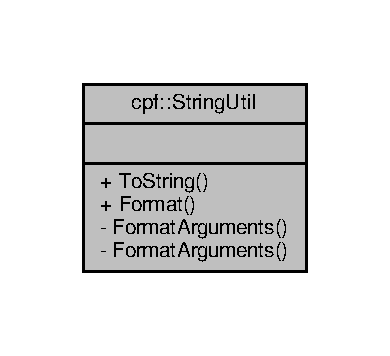
\includegraphics[width=187pt]{classcpf_1_1_string_util__coll__graph}
\end{center}
\end{figure}
\subsection*{정적 Public 멤버 함수}
\begin{DoxyCompactItemize}
\item 
{\footnotesize template$<$typename T $>$ }\\static std\+::string \hyperlink{classcpf_1_1_string_util_a53a8571bef952fecc7008f309171b8c5}{To\+String} (const T \&arg)
\item 
{\footnotesize template$<$typename ... Args$>$ }\\static \hyperlink{namespacecpf_a4dbd6992c3ed4440ce7ed8982ff7ffea}{String} \hyperlink{classcpf_1_1_string_util_a965cca44ea396f01f2f3c5e3851f1001}{Format} (const \hyperlink{namespacecpf_a4dbd6992c3ed4440ce7ed8982ff7ffea}{String} \&fmt, Args \&\&...arguments)
\begin{DoxyCompactList}\small\item\em \{\} =$>$ 해당 순서에 맞는 인자를 대입시킵니다. \{n\} =$>$ n에 해당하는 순서에 맞는 인자를 대입시킵니다. \end{DoxyCompactList}\end{DoxyCompactItemize}
\subsection*{정적 Private 멤버 함수}
\begin{DoxyCompactItemize}
\item 
{\footnotesize template$<$size\+\_\+t Count$>$ }\\static void \hyperlink{classcpf_1_1_string_util_af6a0483e9f189a49f9f25a6ca74d94a2}{Format\+Arguments} (std\+::array$<$ std\+::string, Count $>$ \&fmt)
\item 
{\footnotesize template$<$size\+\_\+t Count, typename T , typename... Args$>$ }\\static void \hyperlink{classcpf_1_1_string_util_a42ad0dd4e29fef98117340ae1193cd95}{Format\+Arguments} (std\+::array$<$ std\+::string, Count $>$ \&fmt, T \&\&arg, Args \&\&...args)
\end{DoxyCompactItemize}


\subsection{상세한 설명}


String.\+hpp 파일의 24 번째 라인에서 정의되었습니다.



\subsection{멤버 함수 문서화}
\mbox{\Hypertarget{classcpf_1_1_string_util_a965cca44ea396f01f2f3c5e3851f1001}\label{classcpf_1_1_string_util_a965cca44ea396f01f2f3c5e3851f1001}} 
\index{cpf\+::\+String\+Util@{cpf\+::\+String\+Util}!Format@{Format}}
\index{Format@{Format}!cpf\+::\+String\+Util@{cpf\+::\+String\+Util}}
\subsubsection{\texorpdfstring{Format()}{Format()}}
{\footnotesize\ttfamily template$<$typename ... Args$>$ \\
static \hyperlink{namespacecpf_a4dbd6992c3ed4440ce7ed8982ff7ffea}{String} cpf\+::\+String\+Util\+::\+Format (\begin{DoxyParamCaption}\item[{const \hyperlink{namespacecpf_a4dbd6992c3ed4440ce7ed8982ff7ffea}{String} \&}]{fmt,  }\item[{Args \&\&...}]{arguments }\end{DoxyParamCaption})\hspace{0.3cm}{\ttfamily [inline]}, {\ttfamily [static]}}



\{\} =$>$ 해당 순서에 맞는 인자를 대입시킵니다. \{n\} =$>$ n에 해당하는 순서에 맞는 인자를 대입시킵니다. 

주어진 포멧에 맞게 인자들을 재배치시킵니다. \begin{DoxyRefDesc}{할일}
\item[\hyperlink{todo__todo000002}{할일}]해당 위치에 특정한 타입으로 대입 시킬 수 있는 포멧을 추가할 예정입니다. \end{DoxyRefDesc}


String.\+hpp 파일의 55 번째 라인에서 정의되었습니다.


\begin{DoxyCode}
55                                                                     \{
56             std::array<std::string, \textcolor{keyword}{sizeof}...(Args)> args;
57             \hyperlink{classcpf_1_1_string_util_af6a0483e9f189a49f9f25a6ca74d94a2}{FormatArguments}(args, std::forward<Args>(arguments)...);
58 
59             \textcolor{keyword}{auto} check = [&fmt](String::const\_iterator it, std::function<bool(const char &ch)> fn) \{
60                 \textcolor{keywordflow}{return} it != fmt.end() && fn(*it);
61             \};
62 
63             \hyperlink{namespacecpf_a6e5583a51165e808f1a480563a2d98b2}{StringStream} ss;
64             \hyperlink{namespacecpf_a6e5583a51165e808f1a480563a2d98b2}{StringStream} tmp;
65             uint32\_t forceOfNature = 0;
66 
67             \textcolor{keywordflow}{for} (String::const\_iterator it = fmt.begin(); it != fmt.end();) \{
68                 \textcolor{keywordflow}{if} (check(it, [](\textcolor{keyword}{const} \textcolor{keywordtype}{char} &ch) -> \textcolor{keywordtype}{bool} \{ \textcolor{keywordflow}{return} ch == \textcolor{charliteral}{'\{'}; \})) \{
69                     it++;
70                     tmp.str(\textcolor{stringliteral}{""});
71 
72                     \textcolor{comment}{// check args}
73                     \textcolor{keywordflow}{while} (check(it, [](\textcolor{keyword}{const} \textcolor{keywordtype}{char} &ch) -> \textcolor{keywordtype}{bool} \{ \textcolor{keywordflow}{return} std::isdigit(ch); \})) \{
74                         tmp << *it;
75                         it++;
76                     \}
77 
78                     \textcolor{keywordflow}{if} (tmp.str().empty()) \{
79                         ss << args[forceOfNature];
80                     \} \textcolor{keywordflow}{else} \{
81                         int32\_t index = std::atoi(tmp.str().c\_str());
82                         \textcolor{keywordflow}{if} (index < args.size()) \{
83                             ss << args[index];
84                         \} \textcolor{keywordflow}{else} \{
85                             std::cout << \textcolor{stringliteral}{"ERROR: Out of range!"} << std::endl 
86                                 << \textcolor{stringliteral}{"Request index is "} << index 
87                                 << \textcolor{stringliteral}{", but max args index is "} << args.size() - 1 << std::endl;
88                             \textcolor{keywordflow}{return} \textcolor{stringliteral}{""};
89                         \}
90     
91                     \}
92 
93                     \textcolor{keywordflow}{if} (!check(it++, [](\textcolor{keyword}{const} \textcolor{keywordtype}{char} &ch) -> \textcolor{keywordtype}{bool} \{ \textcolor{keywordflow}{return} ch == \textcolor{charliteral}{'\}'}; \})) \{
94                         std::cout << \textcolor{stringliteral}{"ERROR: Invalid token! "} << *it << std::endl;
95                         \textcolor{keywordflow}{return} \textcolor{stringliteral}{""};
96                     \}
97 
98                     forceOfNature++;
99                 \} \textcolor{keywordflow}{else} \{
100                     ss << *it;
101                     it++;
102                 \}
103             \}
104 
105             \textcolor{keywordflow}{return} ss.str();
106         \}
\end{DoxyCode}
\mbox{\Hypertarget{classcpf_1_1_string_util_af6a0483e9f189a49f9f25a6ca74d94a2}\label{classcpf_1_1_string_util_af6a0483e9f189a49f9f25a6ca74d94a2}} 
\index{cpf\+::\+String\+Util@{cpf\+::\+String\+Util}!Format\+Arguments@{Format\+Arguments}}
\index{Format\+Arguments@{Format\+Arguments}!cpf\+::\+String\+Util@{cpf\+::\+String\+Util}}
\subsubsection{\texorpdfstring{Format\+Arguments()}{FormatArguments()}\hspace{0.1cm}{\footnotesize\ttfamily [1/2]}}
{\footnotesize\ttfamily template$<$size\+\_\+t Count$>$ \\
static void cpf\+::\+String\+Util\+::\+Format\+Arguments (\begin{DoxyParamCaption}\item[{std\+::array$<$ std\+::string, Count $>$ \&}]{fmt }\end{DoxyParamCaption})\hspace{0.3cm}{\ttfamily [inline]}, {\ttfamily [static]}, {\ttfamily [private]}}



String.\+hpp 파일의 27 번째 라인에서 정의되었습니다.


\begin{DoxyCode}
27                                                                             \{
28             \textcolor{comment}{// base}
29         \}
\end{DoxyCode}
\mbox{\Hypertarget{classcpf_1_1_string_util_a42ad0dd4e29fef98117340ae1193cd95}\label{classcpf_1_1_string_util_a42ad0dd4e29fef98117340ae1193cd95}} 
\index{cpf\+::\+String\+Util@{cpf\+::\+String\+Util}!Format\+Arguments@{Format\+Arguments}}
\index{Format\+Arguments@{Format\+Arguments}!cpf\+::\+String\+Util@{cpf\+::\+String\+Util}}
\subsubsection{\texorpdfstring{Format\+Arguments()}{FormatArguments()}\hspace{0.1cm}{\footnotesize\ttfamily [2/2]}}
{\footnotesize\ttfamily template$<$size\+\_\+t Count, typename T , typename... Args$>$ \\
static void cpf\+::\+String\+Util\+::\+Format\+Arguments (\begin{DoxyParamCaption}\item[{std\+::array$<$ std\+::string, Count $>$ \&}]{fmt,  }\item[{T \&\&}]{arg,  }\item[{Args \&\&...}]{args }\end{DoxyParamCaption})\hspace{0.3cm}{\ttfamily [inline]}, {\ttfamily [static]}, {\ttfamily [private]}}



String.\+hpp 파일의 32 번째 라인에서 정의되었습니다.


\begin{DoxyCode}
32                                                                                                     \{
33             fmt[Count - 1 - \textcolor{keyword}{sizeof}...(args)] = \hyperlink{classcpf_1_1_string_util_a53a8571bef952fecc7008f309171b8c5}{ToString}(arg);
34             \hyperlink{classcpf_1_1_string_util_af6a0483e9f189a49f9f25a6ca74d94a2}{FormatArguments}(fmt, std::forward<Args>(args)...);
35         \}
\end{DoxyCode}
\mbox{\Hypertarget{classcpf_1_1_string_util_a53a8571bef952fecc7008f309171b8c5}\label{classcpf_1_1_string_util_a53a8571bef952fecc7008f309171b8c5}} 
\index{cpf\+::\+String\+Util@{cpf\+::\+String\+Util}!To\+String@{To\+String}}
\index{To\+String@{To\+String}!cpf\+::\+String\+Util@{cpf\+::\+String\+Util}}
\subsubsection{\texorpdfstring{To\+String()}{ToString()}}
{\footnotesize\ttfamily template$<$typename T $>$ \\
static std\+::string cpf\+::\+String\+Util\+::\+To\+String (\begin{DoxyParamCaption}\item[{const T \&}]{arg }\end{DoxyParamCaption})\hspace{0.3cm}{\ttfamily [inline]}, {\ttfamily [static]}}



String.\+hpp 파일의 39 번째 라인에서 정의되었습니다.


\begin{DoxyCode}
39                                                        \{
40             \hyperlink{namespacecpf_a6e5583a51165e808f1a480563a2d98b2}{StringStream} ss;
41             ss << arg;
42             \textcolor{keywordflow}{return} ss.str();
43         \}
\end{DoxyCode}


이 클래스에 대한 문서화 페이지는 다음의 파일로부터 생성되었습니다.\+:\begin{DoxyCompactItemize}
\item 
Source/\+Foundation/\+String/\hyperlink{_string_8hpp}{String.\+hpp}\end{DoxyCompactItemize}

\hypertarget{classcpf_1_1_t_module}{}\section{cpf\+:\+:T\+Module$<$ T $>$ 클래스 템플릿 참조}
\label{classcpf_1_1_t_module}\index{cpf\+::\+T\+Module$<$ T $>$@{cpf\+::\+T\+Module$<$ T $>$}}


{\ttfamily \#include $<$Module.\+hpp$>$}



cpf\+:\+:T\+Module$<$ T $>$에 대한 상속 다이어그램 \+: \nopagebreak
\begin{figure}[H]
\begin{center}
\leavevmode
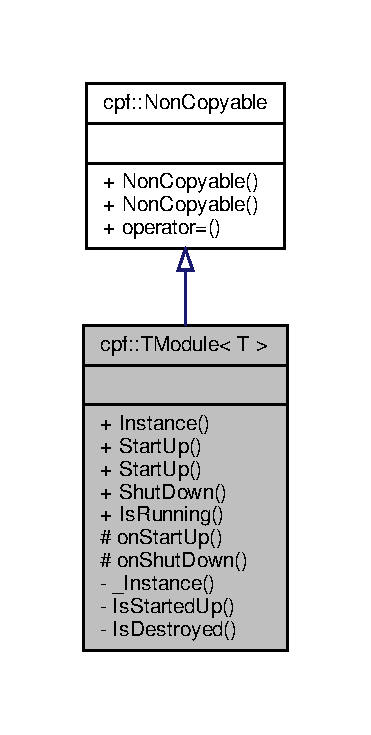
\includegraphics[width=178pt]{classcpf_1_1_t_module__inherit__graph}
\end{center}
\end{figure}


cpf\+:\+:T\+Module$<$ T $>$에 대한 협력 다이어그램\+:\nopagebreak
\begin{figure}[H]
\begin{center}
\leavevmode
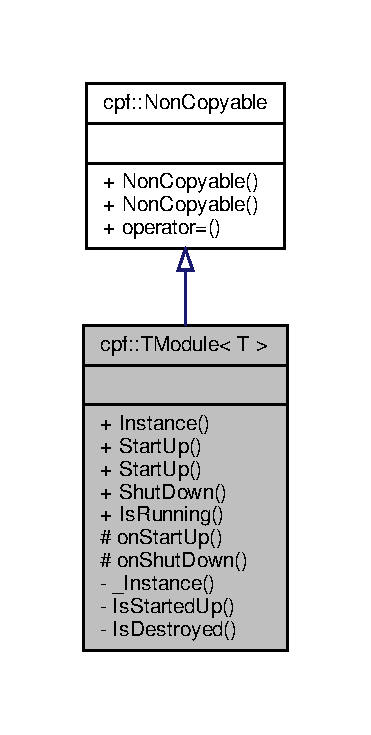
\includegraphics[width=178pt]{classcpf_1_1_t_module__coll__graph}
\end{center}
\end{figure}
\subsection*{정적 Public 멤버 함수}
\begin{DoxyCompactItemize}
\item 
static T \& \hyperlink{classcpf_1_1_t_module_ac8065254584cb0a6656c42f96859d190}{Instance} ()
\item 
{\footnotesize template$<$class ... Args$>$ }\\static void \hyperlink{classcpf_1_1_t_module_a02fbf3c4d28a3328e81b0e8d0bdd93b0}{Start\+Up} (Args \&\&...args)
\item 
{\footnotesize template$<$typename U , class ... Args$>$ }\\static void \hyperlink{classcpf_1_1_t_module_ac553266ad6255da045ef3f34b0f9bc16}{Start\+Up} (Args \&\&...args)
\item 
static void \hyperlink{classcpf_1_1_t_module_a61452801c61e2546b75a7a6a545e82ee}{Shut\+Down} ()
\item 
static bool \hyperlink{classcpf_1_1_t_module_acd38943803d522ba6dcf7f0871b2f502}{Is\+Running} ()
\end{DoxyCompactItemize}
\subsection*{Protected 멤버 함수}
\begin{DoxyCompactItemize}
\item 
virtual void \hyperlink{classcpf_1_1_t_module_a4eb83b0848794e422d2d345439f51a04}{on\+Start\+Up} ()
\item 
virtual void \hyperlink{classcpf_1_1_t_module_a15c93b1aca54022e145961bea8e3ea7d}{on\+Shut\+Down} ()
\end{DoxyCompactItemize}
\subsection*{정적 Private 멤버 함수}
\begin{DoxyCompactItemize}
\item 
static T $\ast$\& \hyperlink{classcpf_1_1_t_module_a06ab8af8ea6b294959937fd2bbc1e615}{\+\_\+\+Instance} ()
\item 
static bool \& \hyperlink{classcpf_1_1_t_module_a73732afee7131dad652bf3e00c75cef9}{Is\+Started\+Up} ()
\item 
static bool \& \hyperlink{classcpf_1_1_t_module_a9f70f0a70ac59b13b7a874f82c877337}{Is\+Destroyed} ()
\end{DoxyCompactItemize}


\subsection{상세한 설명}
\subsubsection*{template$<$typename T$>$\newline
class cpf\+::\+T\+Module$<$ T $>$}

하나의 엔진 모듈입니다. 본질은 특수한 유형의 싱글톤이라 사용 전후에 직접 생성하고 종료해야합니다. 

Module.\+hpp 파일의 21 번째 라인에서 정의되었습니다.



\subsection{멤버 함수 문서화}
\mbox{\Hypertarget{classcpf_1_1_t_module_a06ab8af8ea6b294959937fd2bbc1e615}\label{classcpf_1_1_t_module_a06ab8af8ea6b294959937fd2bbc1e615}} 
\index{cpf\+::\+T\+Module@{cpf\+::\+T\+Module}!\+\_\+\+Instance@{\+\_\+\+Instance}}
\index{\+\_\+\+Instance@{\+\_\+\+Instance}!cpf\+::\+T\+Module@{cpf\+::\+T\+Module}}
\subsubsection{\texorpdfstring{\+\_\+\+Instance()}{\_Instance()}}
{\footnotesize\ttfamily template$<$typename T$>$ \\
static T$\ast$\& \hyperlink{classcpf_1_1_t_module}{cpf\+::\+T\+Module}$<$ T $>$\+::\+\_\+\+Instance (\begin{DoxyParamCaption}{ }\end{DoxyParamCaption})\hspace{0.3cm}{\ttfamily [inline]}, {\ttfamily [static]}, {\ttfamily [private]}}



Module.\+hpp 파일의 126 번째 라인에서 정의되었습니다.


\begin{DoxyCode}
126                                \{
127 \textcolor{preprocessor}{#if COMPILE == COMPILER\_MSVC}
128             \textcolor{keyword}{static} T *inst = \textcolor{keyword}{nullptr};
129             \textcolor{keywordflow}{return} inst;
130 \textcolor{preprocessor}{#else }
131             \textcolor{keywordflow}{return} mInstance;
132 \textcolor{preprocessor}{#endif}
133         \}
\end{DoxyCode}
\mbox{\Hypertarget{classcpf_1_1_t_module_ac8065254584cb0a6656c42f96859d190}\label{classcpf_1_1_t_module_ac8065254584cb0a6656c42f96859d190}} 
\index{cpf\+::\+T\+Module@{cpf\+::\+T\+Module}!Instance@{Instance}}
\index{Instance@{Instance}!cpf\+::\+T\+Module@{cpf\+::\+T\+Module}}
\subsubsection{\texorpdfstring{Instance()}{Instance()}}
{\footnotesize\ttfamily template$<$typename T$>$ \\
static T\& \hyperlink{classcpf_1_1_t_module}{cpf\+::\+T\+Module}$<$ T $>$\+::Instance (\begin{DoxyParamCaption}{ }\end{DoxyParamCaption})\hspace{0.3cm}{\ttfamily [inline]}, {\ttfamily [static]}}

모듈 객체의 참조를 반환합니다. \begin{DoxyWarning}{경고}
모듈이 실행중이 아니라면 에러를 출력하고 프로그램이 종료됩니다. 
\end{DoxyWarning}


Module.\+hpp 파일의 32 번째 라인에서 정의되었습니다.


\begin{DoxyCode}
32                              \{
33             \textcolor{keywordflow}{if} (!\hyperlink{classcpf_1_1_t_module_a73732afee7131dad652bf3e00c75cef9}{IsStartedUp}()) \{
34                 \hyperlink{classcpf_1_1_debug_a22849847c74bcb444922c263c9ae6183}{Debug::LogFatal}(\textcolor{stringliteral}{"Trying to access not start module!"});
35             \}
36 
37             \textcolor{keywordflow}{if} (\hyperlink{classcpf_1_1_t_module_a9f70f0a70ac59b13b7a874f82c877337}{IsDestroyed}()) \{
38                 \hyperlink{classcpf_1_1_debug_a22849847c74bcb444922c263c9ae6183}{Debug::LogFatal}(\textcolor{stringliteral}{"Trying to access destroyed module!"});
39             \}
40 
41             \textcolor{keywordflow}{return} *\hyperlink{classcpf_1_1_t_module_a06ab8af8ea6b294959937fd2bbc1e615}{\_Instance}();
42         \}
\end{DoxyCode}
\mbox{\Hypertarget{classcpf_1_1_t_module_a9f70f0a70ac59b13b7a874f82c877337}\label{classcpf_1_1_t_module_a9f70f0a70ac59b13b7a874f82c877337}} 
\index{cpf\+::\+T\+Module@{cpf\+::\+T\+Module}!Is\+Destroyed@{Is\+Destroyed}}
\index{Is\+Destroyed@{Is\+Destroyed}!cpf\+::\+T\+Module@{cpf\+::\+T\+Module}}
\subsubsection{\texorpdfstring{Is\+Destroyed()}{IsDestroyed()}}
{\footnotesize\ttfamily template$<$typename T$>$ \\
static bool\& \hyperlink{classcpf_1_1_t_module}{cpf\+::\+T\+Module}$<$ T $>$\+::Is\+Destroyed (\begin{DoxyParamCaption}{ }\end{DoxyParamCaption})\hspace{0.3cm}{\ttfamily [inline]}, {\ttfamily [static]}, {\ttfamily [private]}}



Module.\+hpp 파일의 144 번째 라인에서 정의되었습니다.


\begin{DoxyCode}
144                                    \{
145 \textcolor{preprocessor}{#if COMPILE == COMPILER\_MSVC }
146             \textcolor{keyword}{static} \textcolor{keywordtype}{bool} inst = \textcolor{keyword}{false};
147             \textcolor{keywordflow}{return} inst;
148 \textcolor{preprocessor}{#else}
149             \textcolor{keywordflow}{return} mIsDestroyed;
150 \textcolor{preprocessor}{#endif}
151         \}
\end{DoxyCode}
\mbox{\Hypertarget{classcpf_1_1_t_module_acd38943803d522ba6dcf7f0871b2f502}\label{classcpf_1_1_t_module_acd38943803d522ba6dcf7f0871b2f502}} 
\index{cpf\+::\+T\+Module@{cpf\+::\+T\+Module}!Is\+Running@{Is\+Running}}
\index{Is\+Running@{Is\+Running}!cpf\+::\+T\+Module@{cpf\+::\+T\+Module}}
\subsubsection{\texorpdfstring{Is\+Running()}{IsRunning()}}
{\footnotesize\ttfamily template$<$typename T$>$ \\
static bool \hyperlink{classcpf_1_1_t_module}{cpf\+::\+T\+Module}$<$ T $>$\+::Is\+Running (\begin{DoxyParamCaption}{ }\end{DoxyParamCaption})\hspace{0.3cm}{\ttfamily [inline]}, {\ttfamily [static]}}

모듈이 실행 중인지 확인합니다. 

Module.\+hpp 파일의 108 번째 라인에서 정의되었습니다.


\begin{DoxyCode}
108                                 \{
109             \textcolor{keywordflow}{return} \hyperlink{classcpf_1_1_t_module_a73732afee7131dad652bf3e00c75cef9}{IsStartedUp}() && !\hyperlink{classcpf_1_1_t_module_a9f70f0a70ac59b13b7a874f82c877337}{IsDestroyed}();
110         \}
\end{DoxyCode}
\mbox{\Hypertarget{classcpf_1_1_t_module_a73732afee7131dad652bf3e00c75cef9}\label{classcpf_1_1_t_module_a73732afee7131dad652bf3e00c75cef9}} 
\index{cpf\+::\+T\+Module@{cpf\+::\+T\+Module}!Is\+Started\+Up@{Is\+Started\+Up}}
\index{Is\+Started\+Up@{Is\+Started\+Up}!cpf\+::\+T\+Module@{cpf\+::\+T\+Module}}
\subsubsection{\texorpdfstring{Is\+Started\+Up()}{IsStartedUp()}}
{\footnotesize\ttfamily template$<$typename T$>$ \\
static bool\& \hyperlink{classcpf_1_1_t_module}{cpf\+::\+T\+Module}$<$ T $>$\+::Is\+Started\+Up (\begin{DoxyParamCaption}{ }\end{DoxyParamCaption})\hspace{0.3cm}{\ttfamily [inline]}, {\ttfamily [static]}, {\ttfamily [private]}}



Module.\+hpp 파일의 135 번째 라인에서 정의되었습니다.


\begin{DoxyCode}
135                                    \{
136 \textcolor{preprocessor}{#if COMPILE == COMPILER\_MSVC}
137             \textcolor{keyword}{static} \textcolor{keywordtype}{bool} inst = \textcolor{keyword}{false};
138             \textcolor{keywordflow}{return} inst;
139 \textcolor{preprocessor}{#else}
140             \textcolor{keywordflow}{return} mIsStartedUp;
141 \textcolor{preprocessor}{#endif}
142         \}
\end{DoxyCode}
\mbox{\Hypertarget{classcpf_1_1_t_module_a15c93b1aca54022e145961bea8e3ea7d}\label{classcpf_1_1_t_module_a15c93b1aca54022e145961bea8e3ea7d}} 
\index{cpf\+::\+T\+Module@{cpf\+::\+T\+Module}!on\+Shut\+Down@{on\+Shut\+Down}}
\index{on\+Shut\+Down@{on\+Shut\+Down}!cpf\+::\+T\+Module@{cpf\+::\+T\+Module}}
\subsubsection{\texorpdfstring{on\+Shut\+Down()}{onShutDown()}}
{\footnotesize\ttfamily template$<$typename T$>$ \\
virtual void \hyperlink{classcpf_1_1_t_module}{cpf\+::\+T\+Module}$<$ T $>$\+::on\+Shut\+Down (\begin{DoxyParamCaption}{ }\end{DoxyParamCaption})\hspace{0.3cm}{\ttfamily [inline]}, {\ttfamily [protected]}, {\ttfamily [virtual]}}

모듈 해제 직전에 호출됩니다. \begin{DoxyNote}{주의}
해제 직전에 처리해야할 문제가 있다면 해당 함수를 재정의 하세요. 
\end{DoxyNote}


\hyperlink{classcpf_1_1_application_afa25d5eb462d3d5b1ce19c6d217fe9e7}{cpf\+::\+Application}에서 재구현되었습니다.



Module.\+hpp 파일의 123 번째 라인에서 정의되었습니다.


\begin{DoxyCode}
123 \{\}
\end{DoxyCode}
\mbox{\Hypertarget{classcpf_1_1_t_module_a4eb83b0848794e422d2d345439f51a04}\label{classcpf_1_1_t_module_a4eb83b0848794e422d2d345439f51a04}} 
\index{cpf\+::\+T\+Module@{cpf\+::\+T\+Module}!on\+Start\+Up@{on\+Start\+Up}}
\index{on\+Start\+Up@{on\+Start\+Up}!cpf\+::\+T\+Module@{cpf\+::\+T\+Module}}
\subsubsection{\texorpdfstring{on\+Start\+Up()}{onStartUp()}}
{\footnotesize\ttfamily template$<$typename T$>$ \\
virtual void \hyperlink{classcpf_1_1_t_module}{cpf\+::\+T\+Module}$<$ T $>$\+::on\+Start\+Up (\begin{DoxyParamCaption}{ }\end{DoxyParamCaption})\hspace{0.3cm}{\ttfamily [inline]}, {\ttfamily [protected]}, {\ttfamily [virtual]}}

모듈 생성 직후에 호출됩니다. \begin{DoxyNote}{주의}
할당 직후에 처리해야할 문제가 있다면 해당 함수를 재정의 하세요. 
\end{DoxyNote}


\hyperlink{classcpf_1_1_application_ae8e759c8722c48c45dc3e02446062aec}{cpf\+::\+Application}에서 재구현되었습니다.



Module.\+hpp 파일의 117 번째 라인에서 정의되었습니다.


\begin{DoxyCode}
117 \{\}
\end{DoxyCode}
\mbox{\Hypertarget{classcpf_1_1_t_module_a61452801c61e2546b75a7a6a545e82ee}\label{classcpf_1_1_t_module_a61452801c61e2546b75a7a6a545e82ee}} 
\index{cpf\+::\+T\+Module@{cpf\+::\+T\+Module}!Shut\+Down@{Shut\+Down}}
\index{Shut\+Down@{Shut\+Down}!cpf\+::\+T\+Module@{cpf\+::\+T\+Module}}
\subsubsection{\texorpdfstring{Shut\+Down()}{ShutDown()}}
{\footnotesize\ttfamily template$<$typename T$>$ \\
static void \hyperlink{classcpf_1_1_t_module}{cpf\+::\+T\+Module}$<$ T $>$\+::Shut\+Down (\begin{DoxyParamCaption}{ }\end{DoxyParamCaption})\hspace{0.3cm}{\ttfamily [inline]}, {\ttfamily [static]}}

모듈을 종료합니다. \begin{DoxyWarning}{경고}
모듈이 실행 중이 아니라면 에러를 출력하고 프로그램이 종료됩니다. 
\end{DoxyWarning}


Module.\+hpp 파일의 89 번째 라인에서 정의되었습니다.


\begin{DoxyCode}
89                                \{
90             \textcolor{keywordflow}{if} (!\hyperlink{classcpf_1_1_t_module_a73732afee7131dad652bf3e00c75cef9}{IsStartedUp}()) \{
91                 \hyperlink{classcpf_1_1_debug_a22849847c74bcb444922c263c9ae6183}{Debug::LogFatal}(\textcolor{stringliteral}{"Trying to shut down module start yet"});
92             \}
93 
94             \textcolor{keywordflow}{if} (\hyperlink{classcpf_1_1_t_module_a9f70f0a70ac59b13b7a874f82c877337}{IsDestroyed}()) \{
95                 \hyperlink{classcpf_1_1_debug_a22849847c74bcb444922c263c9ae6183}{Debug::LogFatal}(\textcolor{stringliteral}{"Trying to shut down module already shut down"});
96             \}
97 
98             \textcolor{keyword}{static\_cast<}TModule<T> *\textcolor{keyword}{>}(\hyperlink{classcpf_1_1_t_module_a06ab8af8ea6b294959937fd2bbc1e615}{\_Instance}())->\hyperlink{classcpf_1_1_t_module_a15c93b1aca54022e145961bea8e3ea7d}{onShutDown}();
99             \hyperlink{classcpf_1_1_allocator_af63eadbfa53045d7eede980fd5d15eb4}{Allocator::Free}(\hyperlink{classcpf_1_1_t_module_a06ab8af8ea6b294959937fd2bbc1e615}{\_Instance}());
100 
101             \hyperlink{classcpf_1_1_t_module_a06ab8af8ea6b294959937fd2bbc1e615}{\_Instance}() = \textcolor{keyword}{nullptr};
102             \hyperlink{classcpf_1_1_t_module_a9f70f0a70ac59b13b7a874f82c877337}{IsDestroyed}() = \textcolor{keyword}{true};
103         \}
\end{DoxyCode}
\mbox{\Hypertarget{classcpf_1_1_t_module_a02fbf3c4d28a3328e81b0e8d0bdd93b0}\label{classcpf_1_1_t_module_a02fbf3c4d28a3328e81b0e8d0bdd93b0}} 
\index{cpf\+::\+T\+Module@{cpf\+::\+T\+Module}!Start\+Up@{Start\+Up}}
\index{Start\+Up@{Start\+Up}!cpf\+::\+T\+Module@{cpf\+::\+T\+Module}}
\subsubsection{\texorpdfstring{Start\+Up()}{StartUp()}\hspace{0.1cm}{\footnotesize\ttfamily [1/2]}}
{\footnotesize\ttfamily template$<$typename T$>$ \\
template$<$class ... Args$>$ \\
static void \hyperlink{classcpf_1_1_t_module}{cpf\+::\+T\+Module}$<$ T $>$\+::Start\+Up (\begin{DoxyParamCaption}\item[{Args \&\&...}]{args }\end{DoxyParamCaption})\hspace{0.3cm}{\ttfamily [inline]}, {\ttfamily [static]}}

모듈을 주어진 인자와 함께 생성합니다. \begin{DoxyWarning}{경고}
모듈이 실행 중이 아니라면 에러를 출력하고 프로그램이 종료됩니다. 
\end{DoxyWarning}


Module.\+hpp 파일의 50 번째 라인에서 정의되었습니다.


\begin{DoxyCode}
50                                             \{
51             \textcolor{keywordflow}{if} (\hyperlink{classcpf_1_1_t_module_a73732afee7131dad652bf3e00c75cef9}{IsStartedUp}()) \{
52                 \hyperlink{classcpf_1_1_debug_a22849847c74bcb444922c263c9ae6183}{Debug::LogFatal}(\textcolor{stringliteral}{"Trying to start up module already started"});
53             \}
54 
55             \textcolor{keywordflow}{if} (\hyperlink{classcpf_1_1_t_module_a9f70f0a70ac59b13b7a874f82c877337}{IsDestroyed}()) \{
56                 \hyperlink{classcpf_1_1_debug_a22849847c74bcb444922c263c9ae6183}{Debug::LogFatal}(\textcolor{stringliteral}{"Trying to start up module already destroyed"});
57             \}
58 
59             \hyperlink{classcpf_1_1_t_module_a06ab8af8ea6b294959937fd2bbc1e615}{\_Instance}() = Allocator::New<T>(std::forward<Args>(args)...);
60             \textcolor{keyword}{static\_cast<}TModule<T> *\textcolor{keyword}{>}(\hyperlink{classcpf_1_1_t_module_a06ab8af8ea6b294959937fd2bbc1e615}{\_Instance}())->\hyperlink{classcpf_1_1_t_module_a4eb83b0848794e422d2d345439f51a04}{onStartUp}();
61 
62             \hyperlink{classcpf_1_1_t_module_a73732afee7131dad652bf3e00c75cef9}{IsStartedUp}() = \textcolor{keyword}{true};
63         \}
\end{DoxyCode}
\mbox{\Hypertarget{classcpf_1_1_t_module_ac553266ad6255da045ef3f34b0f9bc16}\label{classcpf_1_1_t_module_ac553266ad6255da045ef3f34b0f9bc16}} 
\index{cpf\+::\+T\+Module@{cpf\+::\+T\+Module}!Start\+Up@{Start\+Up}}
\index{Start\+Up@{Start\+Up}!cpf\+::\+T\+Module@{cpf\+::\+T\+Module}}
\subsubsection{\texorpdfstring{Start\+Up()}{StartUp()}\hspace{0.1cm}{\footnotesize\ttfamily [2/2]}}
{\footnotesize\ttfamily template$<$typename T$>$ \\
template$<$typename U , class ... Args$>$ \\
static void \hyperlink{classcpf_1_1_t_module}{cpf\+::\+T\+Module}$<$ T $>$\+::Start\+Up (\begin{DoxyParamCaption}\item[{Args \&\&...}]{args }\end{DoxyParamCaption})\hspace{0.3cm}{\ttfamily [inline]}, {\ttfamily [static]}}

모듈을 주어진 하위 시스템과 인자로 생성합니다. \begin{DoxyWarning}{경고}
모듈이 실행 중이 아니라면 에러를 출력하고 프로그램이 종료됩니다. 
\end{DoxyWarning}


Module.\+hpp 파일의 70 번째 라인에서 정의되었습니다.


\begin{DoxyCode}
70                                             \{
71             \textcolor{keywordflow}{if} (\hyperlink{classcpf_1_1_t_module_a73732afee7131dad652bf3e00c75cef9}{IsStartedUp}()) \{
72                 \hyperlink{classcpf_1_1_debug_a22849847c74bcb444922c263c9ae6183}{Debug::LogFatal}(\textcolor{stringliteral}{"Trying to start up module already started"});
73             \}
74 
75             \textcolor{keywordflow}{if} (\hyperlink{classcpf_1_1_t_module_a9f70f0a70ac59b13b7a874f82c877337}{IsDestroyed}()) \{
76                 \hyperlink{classcpf_1_1_debug_a22849847c74bcb444922c263c9ae6183}{Debug::LogFatal}(\textcolor{stringliteral}{"Trying to start up module already destroyed"});
77             \}
78 
79             \hyperlink{classcpf_1_1_t_module_a06ab8af8ea6b294959937fd2bbc1e615}{\_Instance}() = Allocator::New<U>(std::forward<Args>(args)...);
80             \textcolor{keyword}{static\_cast<}TModule<T> *\textcolor{keyword}{>}(\hyperlink{classcpf_1_1_t_module_a06ab8af8ea6b294959937fd2bbc1e615}{\_Instance}())->\hyperlink{classcpf_1_1_t_module_a15c93b1aca54022e145961bea8e3ea7d}{onShutDown}();
81 
82             \hyperlink{classcpf_1_1_t_module_a73732afee7131dad652bf3e00c75cef9}{IsStartedUp}() = \textcolor{keyword}{true};
83         \}
\end{DoxyCode}


이 클래스에 대한 문서화 페이지는 다음의 파일로부터 생성되었습니다.\+:\begin{DoxyCompactItemize}
\item 
Source/\+Foundation/\+Utility/\hyperlink{_module_8hpp}{Module.\+hpp}\end{DoxyCompactItemize}

\chapter{파일 문서화}
\hypertarget{_system_8hpp}{}\section{Source/\+Foundation/\+Alloc/\+System.hpp 파일 참조}
\label{_system_8hpp}\index{Source/\+Foundation/\+Alloc/\+System.\+hpp@{Source/\+Foundation/\+Alloc/\+System.\+hpp}}
이 그래프는 이 파일을 직/간접적으로 include 하는 파일들을 보여줍니다.\+:
\nopagebreak
\begin{figure}[H]
\begin{center}
\leavevmode
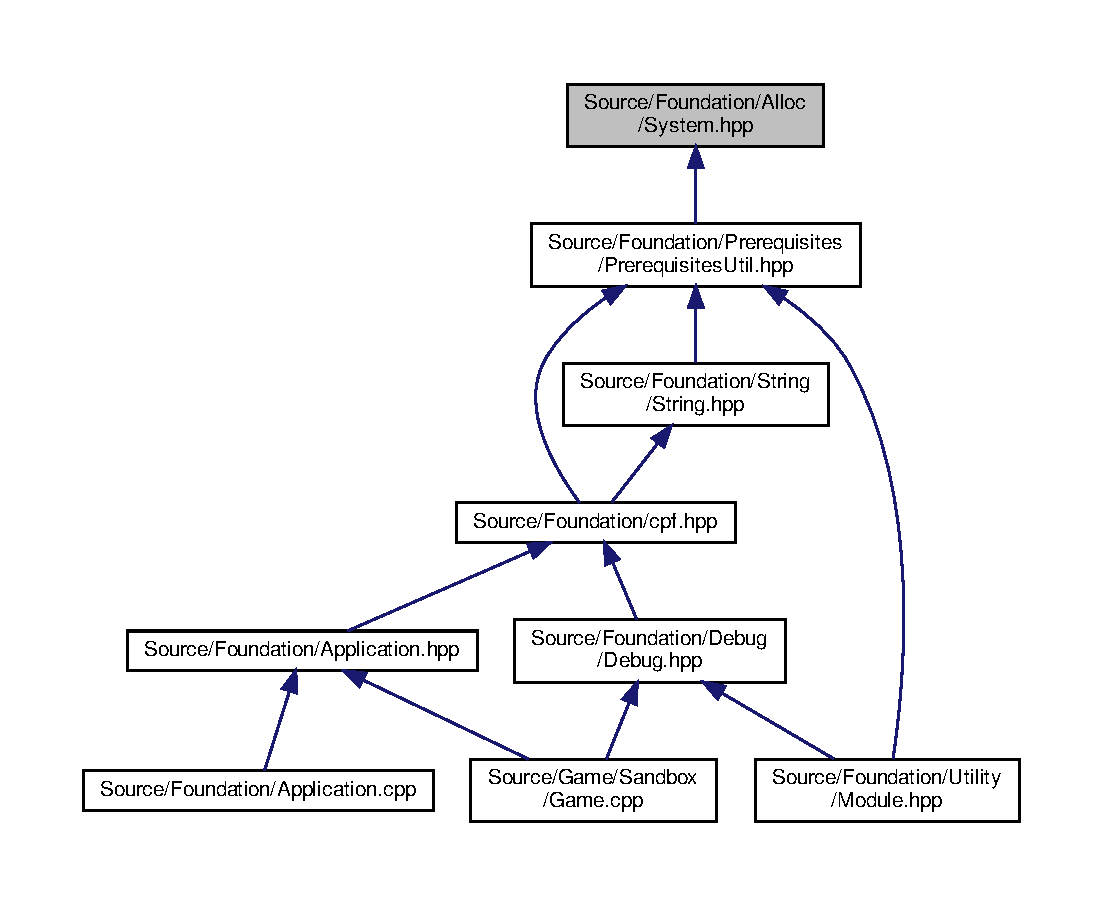
\includegraphics[width=350pt]{_system_8hpp__dep__incl}
\end{center}
\end{figure}
\subsection*{클래스}
\begin{DoxyCompactItemize}
\item 
class \hyperlink{classcpf_1_1_allocator}{cpf\+::\+Allocator}
\end{DoxyCompactItemize}
\subsection*{네임스페이스}
\begin{DoxyCompactItemize}
\item 
 \hyperlink{namespacecpf}{cpf}
\end{DoxyCompactItemize}

\hypertarget{_application_8cpp}{}\section{Source/\+Foundation/\+Application.cpp 파일 참조}
\label{_application_8cpp}\index{Source/\+Foundation/\+Application.\+cpp@{Source/\+Foundation/\+Application.\+cpp}}
{\ttfamily \#include \char`\"{}Application.\+hpp\char`\"{}}\newline
Application.\+cpp에 대한 include 의존 그래프\nopagebreak
\begin{figure}[H]
\begin{center}
\leavevmode
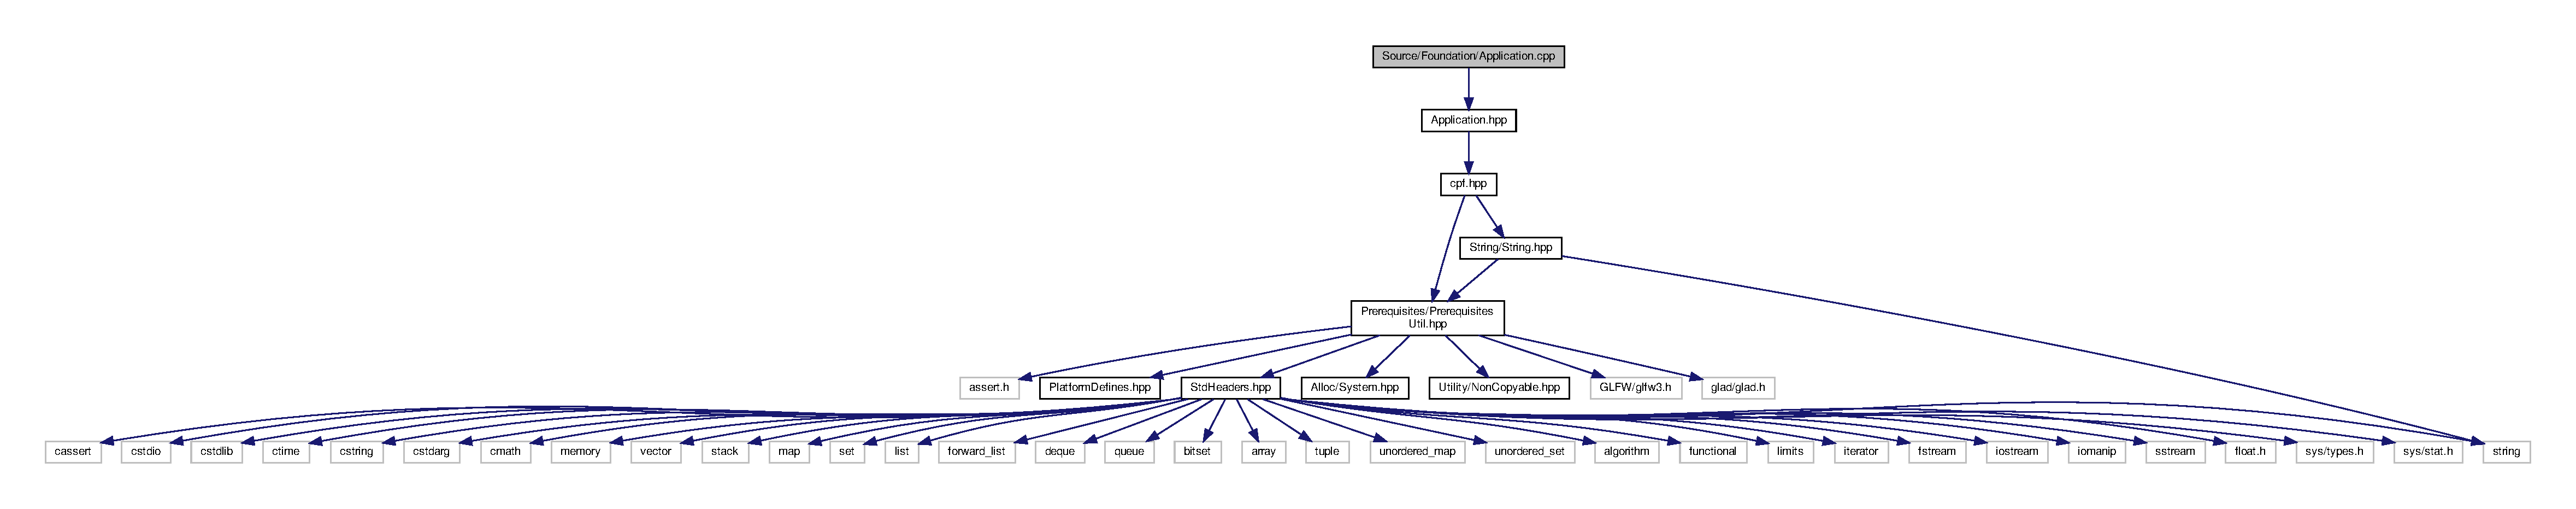
\includegraphics[width=350pt]{_application_8cpp__incl}
\end{center}
\end{figure}
\subsection*{네임스페이스}
\begin{DoxyCompactItemize}
\item 
 \hyperlink{namespacecpf}{cpf}
\end{DoxyCompactItemize}

\hypertarget{_application_8hpp}{}\section{Source/\+Foundation/\+Application.hpp 파일 참조}
\label{_application_8hpp}\index{Source/\+Foundation/\+Application.\+hpp@{Source/\+Foundation/\+Application.\+hpp}}
{\ttfamily \#include \char`\"{}cpf.\+hpp\char`\"{}}\newline
{\ttfamily \#include \char`\"{}Rendering/\+Render\+Window.\+hpp\char`\"{}}\newline
{\ttfamily \#include \char`\"{}Utility/\+Module.\+hpp\char`\"{}}\newline
Application.\+hpp에 대한 include 의존 그래프
\nopagebreak
\begin{figure}[H]
\begin{center}
\leavevmode
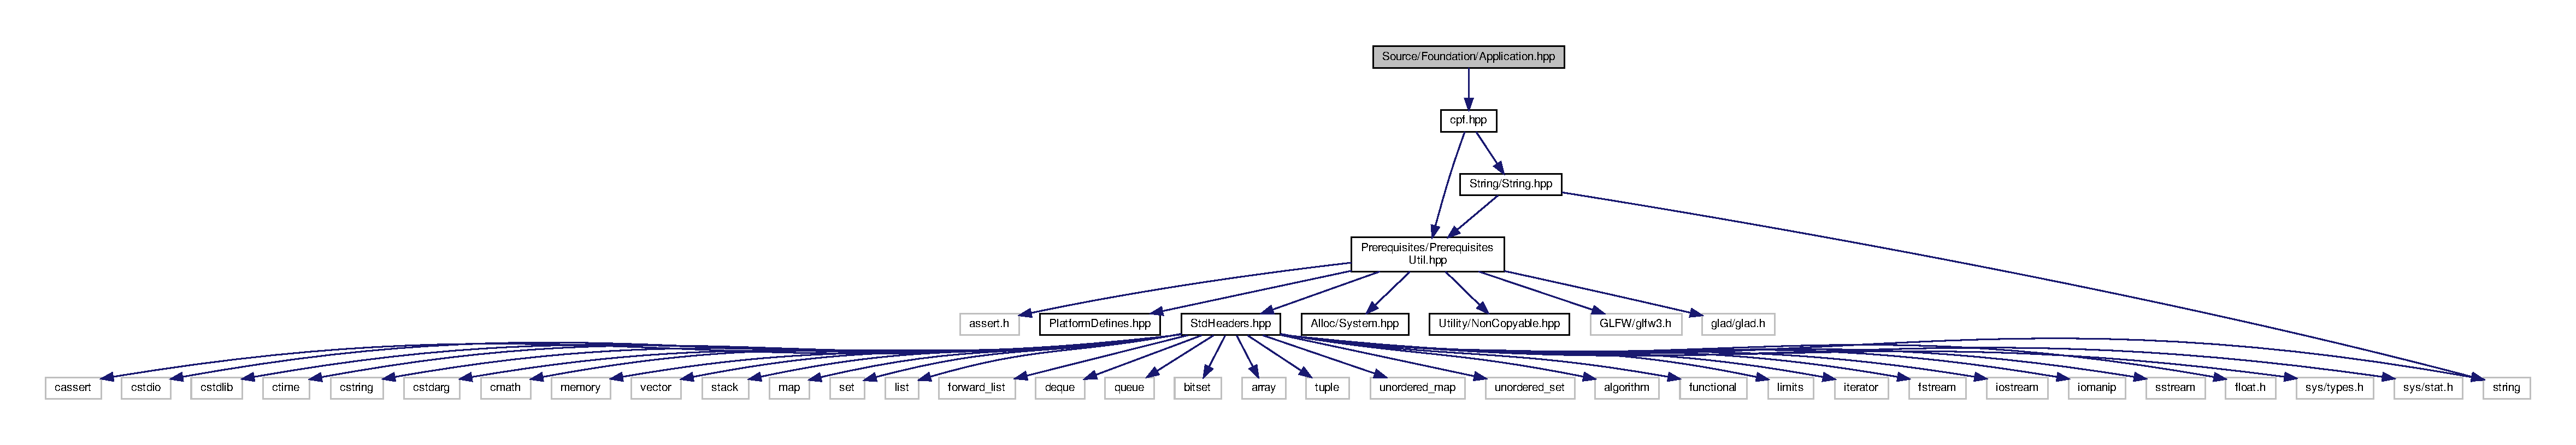
\includegraphics[width=350pt]{_application_8hpp__incl}
\end{center}
\end{figure}
이 그래프는 이 파일을 직/간접적으로 include 하는 파일들을 보여줍니다.\+:
\nopagebreak
\begin{figure}[H]
\begin{center}
\leavevmode
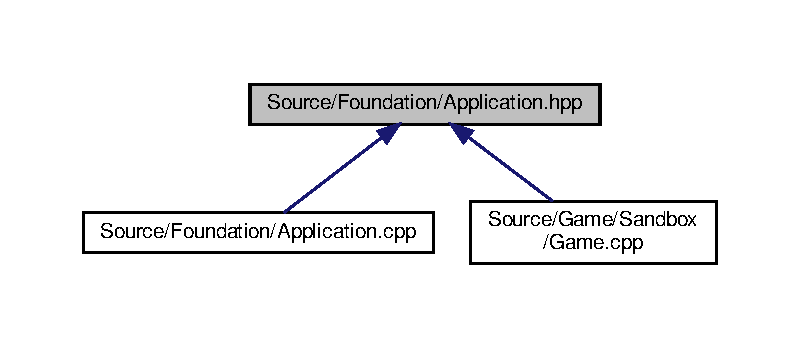
\includegraphics[width=350pt]{_application_8hpp__dep__incl}
\end{center}
\end{figure}
\subsection*{클래스}
\begin{DoxyCompactItemize}
\item 
struct \hyperlink{structcpf_1_1_application_create_info}{cpf\+::\+Application\+Create\+Info}
\item 
class \hyperlink{classcpf_1_1_application}{cpf\+::\+Application}
\end{DoxyCompactItemize}
\subsection*{네임스페이스}
\begin{DoxyCompactItemize}
\item 
 \hyperlink{namespacecpf}{cpf}
\end{DoxyCompactItemize}

\hypertarget{cpf_8hpp}{}\section{Source/\+Foundation/cpf.hpp 파일 참조}
\label{cpf_8hpp}\index{Source/\+Foundation/cpf.\+hpp@{Source/\+Foundation/cpf.\+hpp}}
{\ttfamily \#include \char`\"{}Prerequisites/\+Prerequisites\+Util.\+hpp\char`\"{}}\newline
{\ttfamily \#include \char`\"{}String/\+String.\+hpp\char`\"{}}\newline
cpf.\+hpp에 대한 include 의존 그래프\nopagebreak
\begin{figure}[H]
\begin{center}
\leavevmode
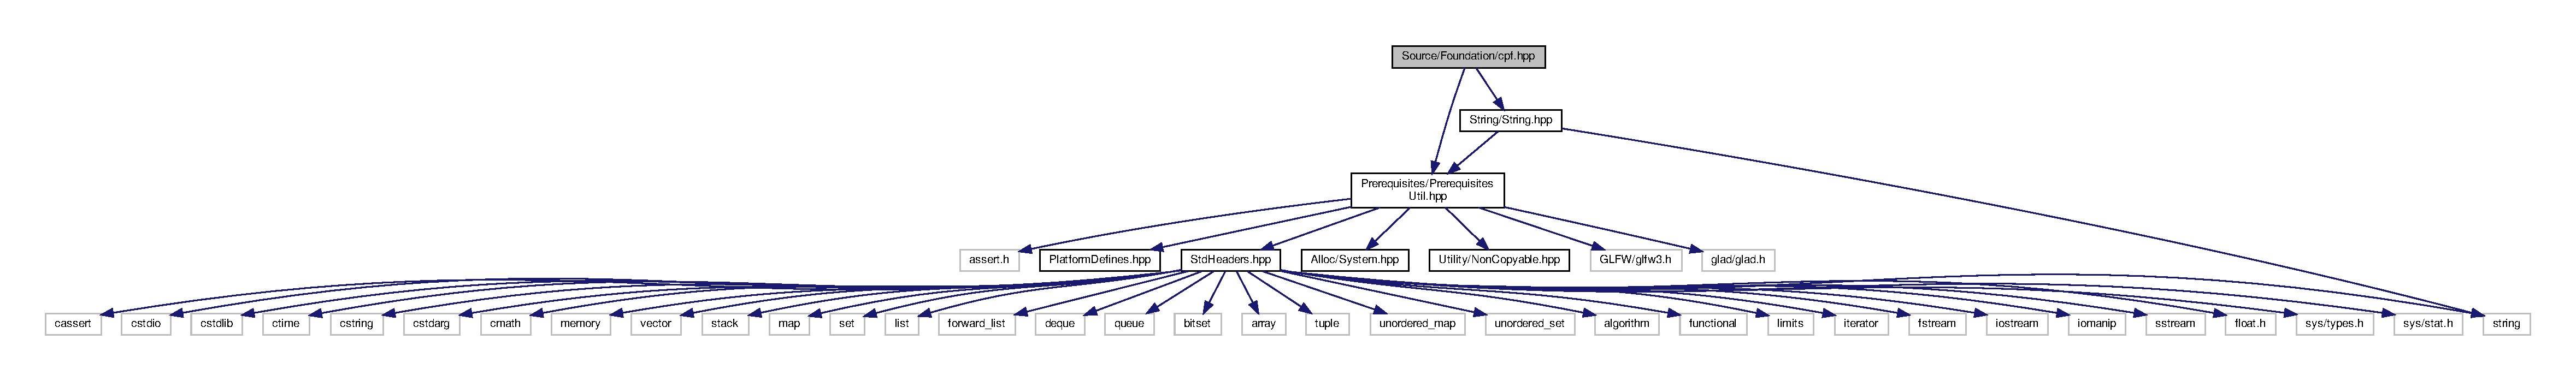
\includegraphics[width=350pt]{cpf_8hpp__incl}
\end{center}
\end{figure}
이 그래프는 이 파일을 직/간접적으로 include 하는 파일들을 보여줍니다.\+:
\nopagebreak
\begin{figure}[H]
\begin{center}
\leavevmode
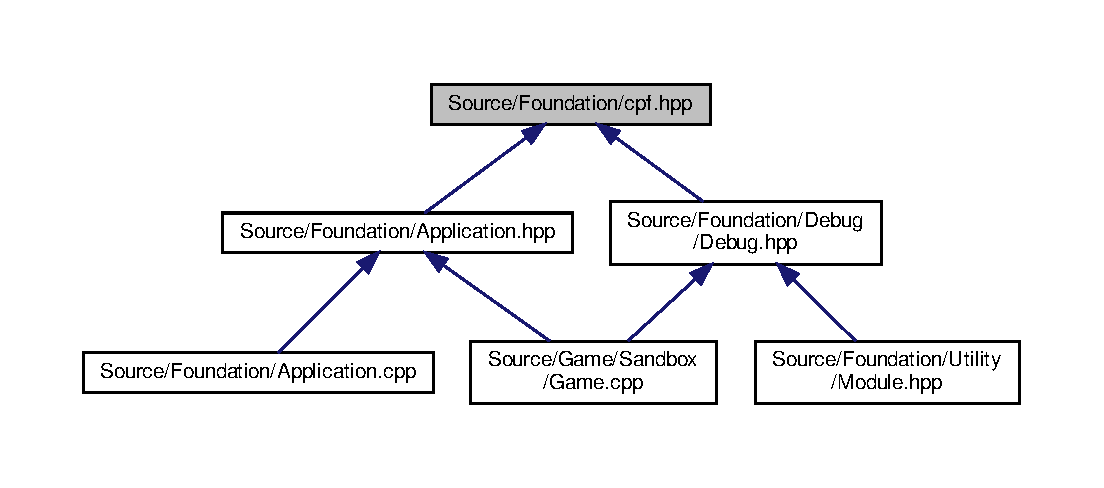
\includegraphics[width=350pt]{cpf_8hpp__dep__incl}
\end{center}
\end{figure}
\subsection*{네임스페이스}
\begin{DoxyCompactItemize}
\item 
 \hyperlink{namespacecpf}{cpf}
\end{DoxyCompactItemize}
\subsection*{타입정의}
\begin{DoxyCompactItemize}
\item 
{\footnotesize template$<$class T $>$ }\\using \hyperlink{namespacecpf_a91e72db639307e12a24546a0eebb1a42}{cpf\+::\+S\+Ptr} = std\+::shared\+\_\+ptr$<$ T $>$
\item 
{\footnotesize template$<$class T $>$ }\\using \hyperlink{namespacecpf_ae8ac5e55927cc357960f1d47c19fe0b9}{cpf\+::\+U\+Ptr} = std\+::unique\+\_\+ptr$<$ T $>$
\item 
using \hyperlink{namespacecpf_a3f0ea2ea743b0adb7c12e52131d485b5}{cpf\+::\+H\+Render\+Target} = S\+Ptr$<$ Render\+Target $>$
\item 
using \hyperlink{namespacecpf_af5ffcc39bb6465427fc3b91366c917f6}{cpf\+::\+H\+Render\+Window} = S\+Ptr$<$ Render\+Window $>$
\end{DoxyCompactItemize}

\hypertarget{_debug_8cpp}{}\section{Source/\+Foundation/\+Debug/\+Debug.cpp 파일 참조}
\label{_debug_8cpp}\index{Source/\+Foundation/\+Debug/\+Debug.\+cpp@{Source/\+Foundation/\+Debug/\+Debug.\+cpp}}

\hypertarget{_debug_8hpp}{}\section{Source/\+Foundation/\+Debug/\+Debug.hpp 파일 참조}
\label{_debug_8hpp}\index{Source/\+Foundation/\+Debug/\+Debug.\+hpp@{Source/\+Foundation/\+Debug/\+Debug.\+hpp}}
{\ttfamily \#include \char`\"{}cpf.\+hpp\char`\"{}}\newline
Debug.\+hpp에 대한 include 의존 그래프\nopagebreak
\begin{figure}[H]
\begin{center}
\leavevmode
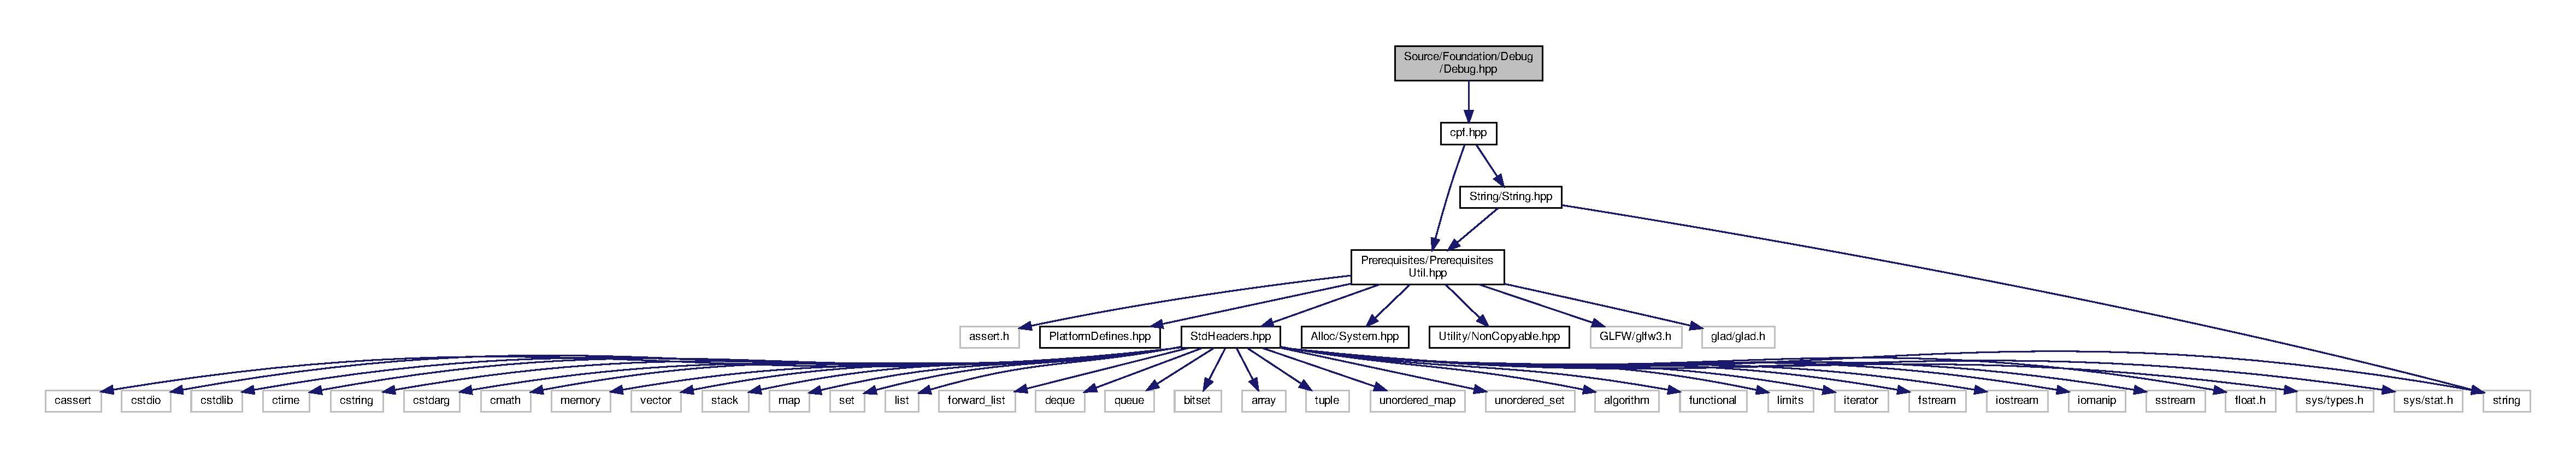
\includegraphics[width=350pt]{_debug_8hpp__incl}
\end{center}
\end{figure}
이 그래프는 이 파일을 직/간접적으로 include 하는 파일들을 보여줍니다.\+:\nopagebreak
\begin{figure}[H]
\begin{center}
\leavevmode
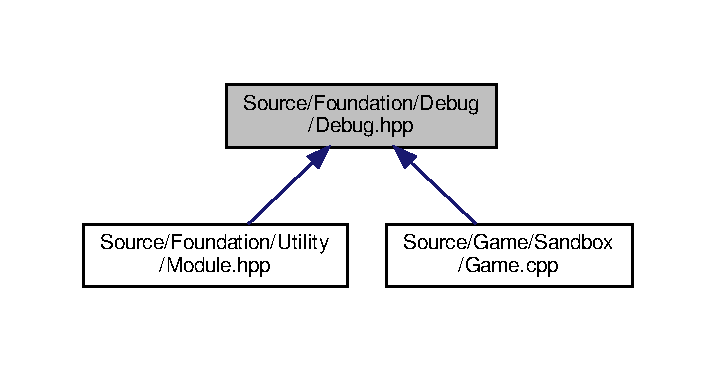
\includegraphics[width=344pt]{_debug_8hpp__dep__incl}
\end{center}
\end{figure}
\subsection*{클래스}
\begin{DoxyCompactItemize}
\item 
class \hyperlink{classcpf_1_1_debug}{cpf\+::\+Debug}
\end{DoxyCompactItemize}
\subsection*{네임스페이스}
\begin{DoxyCompactItemize}
\item 
 \hyperlink{namespacecpf}{cpf}
\end{DoxyCompactItemize}

\hypertarget{_platform_defines_8hpp}{}\section{Source/\+Foundation/\+Prerequisites/\+Platform\+Defines.hpp 파일 참조}
\label{_platform_defines_8hpp}\index{Source/\+Foundation/\+Prerequisites/\+Platform\+Defines.\+hpp@{Source/\+Foundation/\+Prerequisites/\+Platform\+Defines.\+hpp}}
이 그래프는 이 파일을 직/간접적으로 include 하는 파일들을 보여줍니다.\+:\nopagebreak
\begin{figure}[H]
\begin{center}
\leavevmode
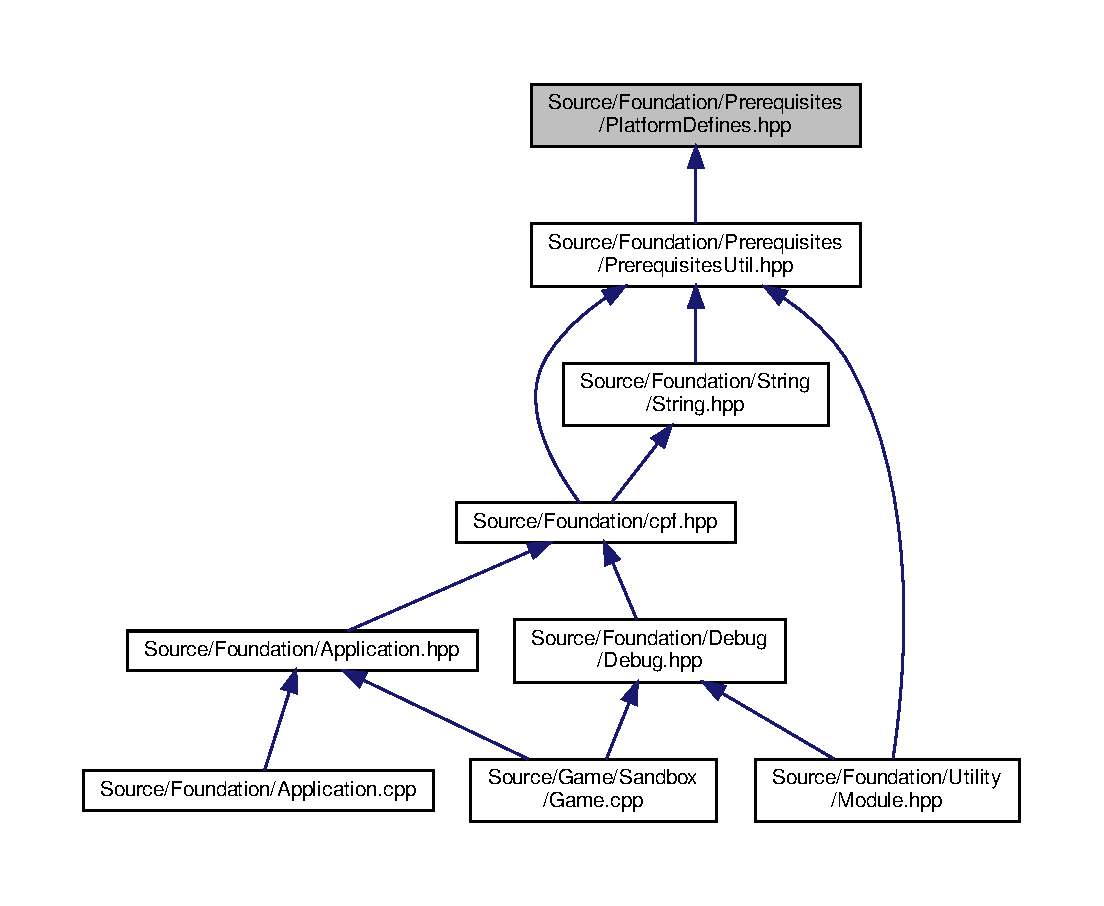
\includegraphics[width=350pt]{_platform_defines_8hpp__dep__incl}
\end{center}
\end{figure}
\subsection*{매크로}
\begin{DoxyCompactItemize}
\item 
\#define \hyperlink{_platform_defines_8hpp_a15efcdea14416b069da71f2c04d9bd08}{P\+L\+A\+T\+F\+O\+R\+M\+\_\+\+W\+I\+N32}~1
\item 
\#define \hyperlink{_platform_defines_8hpp_affcc3790504b838f9ce56a008cce0950}{P\+L\+A\+T\+F\+O\+R\+M\+\_\+\+L\+I\+N\+UX}~2
\item 
\#define \hyperlink{_platform_defines_8hpp_a6277ef2afb55add8d81d32ebd07e1540}{C\+O\+M\+P\+I\+L\+E\+R\+\_\+\+M\+S\+VC}~1
\item 
\#define \hyperlink{_platform_defines_8hpp_a01b57e71dec2e02afbc8021a4b7bae29}{C\+O\+M\+P\+I\+L\+E\+R\+\_\+\+G\+N\+UC}~2
\item 
\#define \hyperlink{_platform_defines_8hpp_a6b57fb2a693b8ae06b593c7614cb0c7f}{C\+O\+M\+P\+I\+L\+E\+R\+\_\+\+C\+L\+A\+NG}~3
\item 
\#define \hyperlink{_platform_defines_8hpp_a1fa4f1561216be34f745f32aaa38d943}{P\+L\+A\+T\+F\+O\+RM}~\hyperlink{_platform_defines_8hpp_affcc3790504b838f9ce56a008cce0950}{P\+L\+A\+T\+F\+O\+R\+M\+\_\+\+L\+I\+N\+UX}
\item 
\#define \hyperlink{_platform_defines_8hpp_a1ca888bd091694c05472e1b91df1a97b}{D\+L\+L\+\_\+\+E\+X\+P\+O\+RT}~\+\_\+\+\_\+attribute\+\_\+\+\_\+ ((visibility(\char`\"{}default\char`\"{})))
\item 
\#define \hyperlink{_platform_defines_8hpp_a89cec5a0cc184865c34c13ae6a0481fb}{P\+L\+U\+G\+I\+N\+\_\+\+E\+X\+P\+O\+RT}~\+\_\+\+\_\+attribute\+\_\+\+\_\+((visibility(\char`\"{}default\char`\"{})))
\end{DoxyCompactItemize}


\subsection{매크로 문서화}
\mbox{\Hypertarget{_platform_defines_8hpp_a6b57fb2a693b8ae06b593c7614cb0c7f}\label{_platform_defines_8hpp_a6b57fb2a693b8ae06b593c7614cb0c7f}} 
\index{Platform\+Defines.\+hpp@{Platform\+Defines.\+hpp}!C\+O\+M\+P\+I\+L\+E\+R\+\_\+\+C\+L\+A\+NG@{C\+O\+M\+P\+I\+L\+E\+R\+\_\+\+C\+L\+A\+NG}}
\index{C\+O\+M\+P\+I\+L\+E\+R\+\_\+\+C\+L\+A\+NG@{C\+O\+M\+P\+I\+L\+E\+R\+\_\+\+C\+L\+A\+NG}!Platform\+Defines.\+hpp@{Platform\+Defines.\+hpp}}
\subsubsection{\texorpdfstring{C\+O\+M\+P\+I\+L\+E\+R\+\_\+\+C\+L\+A\+NG}{COMPILER\_CLANG}}
{\footnotesize\ttfamily \#define C\+O\+M\+P\+I\+L\+E\+R\+\_\+\+C\+L\+A\+NG~3}



Platform\+Defines.\+hpp 파일의 8 번째 라인에서 정의되었습니다.

\mbox{\Hypertarget{_platform_defines_8hpp_a01b57e71dec2e02afbc8021a4b7bae29}\label{_platform_defines_8hpp_a01b57e71dec2e02afbc8021a4b7bae29}} 
\index{Platform\+Defines.\+hpp@{Platform\+Defines.\+hpp}!C\+O\+M\+P\+I\+L\+E\+R\+\_\+\+G\+N\+UC@{C\+O\+M\+P\+I\+L\+E\+R\+\_\+\+G\+N\+UC}}
\index{C\+O\+M\+P\+I\+L\+E\+R\+\_\+\+G\+N\+UC@{C\+O\+M\+P\+I\+L\+E\+R\+\_\+\+G\+N\+UC}!Platform\+Defines.\+hpp@{Platform\+Defines.\+hpp}}
\subsubsection{\texorpdfstring{C\+O\+M\+P\+I\+L\+E\+R\+\_\+\+G\+N\+UC}{COMPILER\_GNUC}}
{\footnotesize\ttfamily \#define C\+O\+M\+P\+I\+L\+E\+R\+\_\+\+G\+N\+UC~2}



Platform\+Defines.\+hpp 파일의 7 번째 라인에서 정의되었습니다.

\mbox{\Hypertarget{_platform_defines_8hpp_a6277ef2afb55add8d81d32ebd07e1540}\label{_platform_defines_8hpp_a6277ef2afb55add8d81d32ebd07e1540}} 
\index{Platform\+Defines.\+hpp@{Platform\+Defines.\+hpp}!C\+O\+M\+P\+I\+L\+E\+R\+\_\+\+M\+S\+VC@{C\+O\+M\+P\+I\+L\+E\+R\+\_\+\+M\+S\+VC}}
\index{C\+O\+M\+P\+I\+L\+E\+R\+\_\+\+M\+S\+VC@{C\+O\+M\+P\+I\+L\+E\+R\+\_\+\+M\+S\+VC}!Platform\+Defines.\+hpp@{Platform\+Defines.\+hpp}}
\subsubsection{\texorpdfstring{C\+O\+M\+P\+I\+L\+E\+R\+\_\+\+M\+S\+VC}{COMPILER\_MSVC}}
{\footnotesize\ttfamily \#define C\+O\+M\+P\+I\+L\+E\+R\+\_\+\+M\+S\+VC~1}



Platform\+Defines.\+hpp 파일의 6 번째 라인에서 정의되었습니다.

\mbox{\Hypertarget{_platform_defines_8hpp_a1ca888bd091694c05472e1b91df1a97b}\label{_platform_defines_8hpp_a1ca888bd091694c05472e1b91df1a97b}} 
\index{Platform\+Defines.\+hpp@{Platform\+Defines.\+hpp}!D\+L\+L\+\_\+\+E\+X\+P\+O\+RT@{D\+L\+L\+\_\+\+E\+X\+P\+O\+RT}}
\index{D\+L\+L\+\_\+\+E\+X\+P\+O\+RT@{D\+L\+L\+\_\+\+E\+X\+P\+O\+RT}!Platform\+Defines.\+hpp@{Platform\+Defines.\+hpp}}
\subsubsection{\texorpdfstring{D\+L\+L\+\_\+\+E\+X\+P\+O\+RT}{DLL\_EXPORT}}
{\footnotesize\ttfamily \#define D\+L\+L\+\_\+\+E\+X\+P\+O\+RT~\+\_\+\+\_\+attribute\+\_\+\+\_\+ ((visibility(\char`\"{}default\char`\"{})))}



Platform\+Defines.\+hpp 파일의 43 번째 라인에서 정의되었습니다.

\mbox{\Hypertarget{_platform_defines_8hpp_a1fa4f1561216be34f745f32aaa38d943}\label{_platform_defines_8hpp_a1fa4f1561216be34f745f32aaa38d943}} 
\index{Platform\+Defines.\+hpp@{Platform\+Defines.\+hpp}!P\+L\+A\+T\+F\+O\+RM@{P\+L\+A\+T\+F\+O\+RM}}
\index{P\+L\+A\+T\+F\+O\+RM@{P\+L\+A\+T\+F\+O\+RM}!Platform\+Defines.\+hpp@{Platform\+Defines.\+hpp}}
\subsubsection{\texorpdfstring{P\+L\+A\+T\+F\+O\+RM}{PLATFORM}}
{\footnotesize\ttfamily \#define P\+L\+A\+T\+F\+O\+RM~\hyperlink{_platform_defines_8hpp_affcc3790504b838f9ce56a008cce0950}{P\+L\+A\+T\+F\+O\+R\+M\+\_\+\+L\+I\+N\+UX}}



Platform\+Defines.\+hpp 파일의 24 번째 라인에서 정의되었습니다.

\mbox{\Hypertarget{_platform_defines_8hpp_affcc3790504b838f9ce56a008cce0950}\label{_platform_defines_8hpp_affcc3790504b838f9ce56a008cce0950}} 
\index{Platform\+Defines.\+hpp@{Platform\+Defines.\+hpp}!P\+L\+A\+T\+F\+O\+R\+M\+\_\+\+L\+I\+N\+UX@{P\+L\+A\+T\+F\+O\+R\+M\+\_\+\+L\+I\+N\+UX}}
\index{P\+L\+A\+T\+F\+O\+R\+M\+\_\+\+L\+I\+N\+UX@{P\+L\+A\+T\+F\+O\+R\+M\+\_\+\+L\+I\+N\+UX}!Platform\+Defines.\+hpp@{Platform\+Defines.\+hpp}}
\subsubsection{\texorpdfstring{P\+L\+A\+T\+F\+O\+R\+M\+\_\+\+L\+I\+N\+UX}{PLATFORM\_LINUX}}
{\footnotesize\ttfamily \#define P\+L\+A\+T\+F\+O\+R\+M\+\_\+\+L\+I\+N\+UX~2}



Platform\+Defines.\+hpp 파일의 4 번째 라인에서 정의되었습니다.

\mbox{\Hypertarget{_platform_defines_8hpp_a15efcdea14416b069da71f2c04d9bd08}\label{_platform_defines_8hpp_a15efcdea14416b069da71f2c04d9bd08}} 
\index{Platform\+Defines.\+hpp@{Platform\+Defines.\+hpp}!P\+L\+A\+T\+F\+O\+R\+M\+\_\+\+W\+I\+N32@{P\+L\+A\+T\+F\+O\+R\+M\+\_\+\+W\+I\+N32}}
\index{P\+L\+A\+T\+F\+O\+R\+M\+\_\+\+W\+I\+N32@{P\+L\+A\+T\+F\+O\+R\+M\+\_\+\+W\+I\+N32}!Platform\+Defines.\+hpp@{Platform\+Defines.\+hpp}}
\subsubsection{\texorpdfstring{P\+L\+A\+T\+F\+O\+R\+M\+\_\+\+W\+I\+N32}{PLATFORM\_WIN32}}
{\footnotesize\ttfamily \#define P\+L\+A\+T\+F\+O\+R\+M\+\_\+\+W\+I\+N32~1}



Platform\+Defines.\+hpp 파일의 3 번째 라인에서 정의되었습니다.

\mbox{\Hypertarget{_platform_defines_8hpp_a89cec5a0cc184865c34c13ae6a0481fb}\label{_platform_defines_8hpp_a89cec5a0cc184865c34c13ae6a0481fb}} 
\index{Platform\+Defines.\+hpp@{Platform\+Defines.\+hpp}!P\+L\+U\+G\+I\+N\+\_\+\+E\+X\+P\+O\+RT@{P\+L\+U\+G\+I\+N\+\_\+\+E\+X\+P\+O\+RT}}
\index{P\+L\+U\+G\+I\+N\+\_\+\+E\+X\+P\+O\+RT@{P\+L\+U\+G\+I\+N\+\_\+\+E\+X\+P\+O\+RT}!Platform\+Defines.\+hpp@{Platform\+Defines.\+hpp}}
\subsubsection{\texorpdfstring{P\+L\+U\+G\+I\+N\+\_\+\+E\+X\+P\+O\+RT}{PLUGIN\_EXPORT}}
{\footnotesize\ttfamily \#define P\+L\+U\+G\+I\+N\+\_\+\+E\+X\+P\+O\+RT~\+\_\+\+\_\+attribute\+\_\+\+\_\+((visibility(\char`\"{}default\char`\"{})))}



Platform\+Defines.\+hpp 파일의 53 번째 라인에서 정의되었습니다.


\hypertarget{_prerequisites_util_8hpp}{}\section{Source/\+Foundation/\+Prerequisites/\+Prerequisites\+Util.hpp 파일 참조}
\label{_prerequisites_util_8hpp}\index{Source/\+Foundation/\+Prerequisites/\+Prerequisites\+Util.\+hpp@{Source/\+Foundation/\+Prerequisites/\+Prerequisites\+Util.\+hpp}}
{\ttfamily \#include $<$assert.\+h$>$}\newline
{\ttfamily \#include \char`\"{}Platform\+Defines.\+hpp\char`\"{}}\newline
{\ttfamily \#include \char`\"{}Std\+Headers.\+hpp\char`\"{}}\newline
{\ttfamily \#include \char`\"{}Alloc/\+System.\+hpp\char`\"{}}\newline
{\ttfamily \#include \char`\"{}Utility/\+Non\+Copyable.\+hpp\char`\"{}}\newline
{\ttfamily \#include $<$G\+L\+F\+W/glfw3.\+h$>$}\newline
{\ttfamily \#include $<$glad/glad.\+h$>$}\newline
Prerequisites\+Util.\+hpp에 대한 include 의존 그래프\nopagebreak
\begin{figure}[H]
\begin{center}
\leavevmode
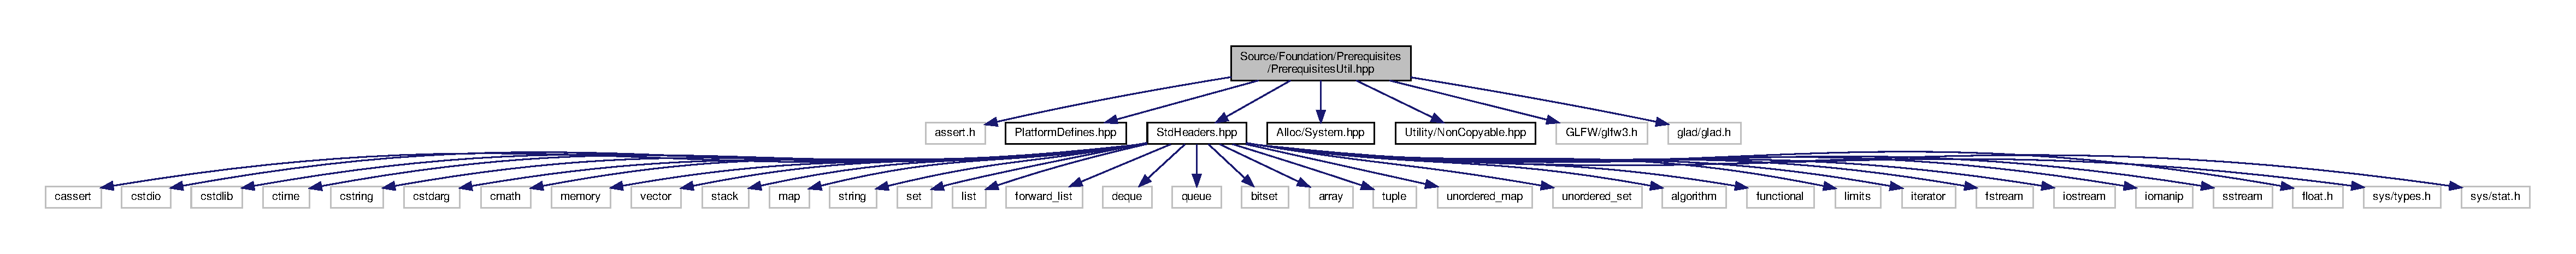
\includegraphics[width=350pt]{_prerequisites_util_8hpp__incl}
\end{center}
\end{figure}
이 그래프는 이 파일을 직/간접적으로 include 하는 파일들을 보여줍니다.\+:\nopagebreak
\begin{figure}[H]
\begin{center}
\leavevmode
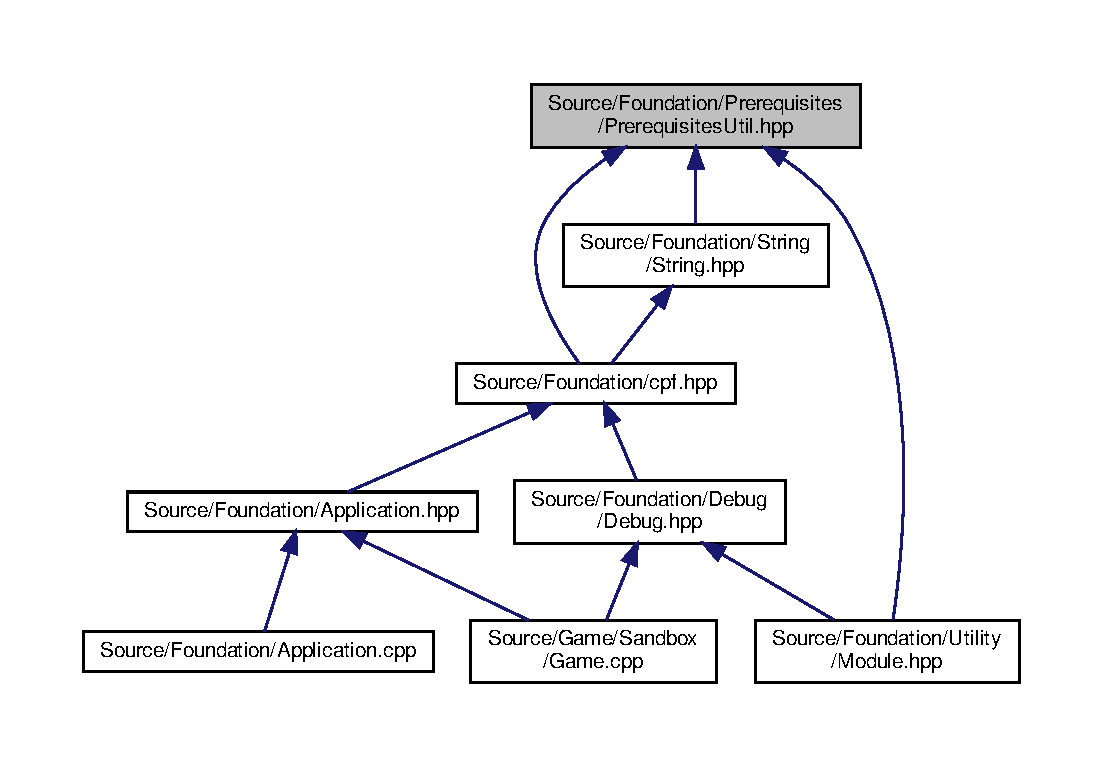
\includegraphics[width=350pt]{_prerequisites_util_8hpp__dep__incl}
\end{center}
\end{figure}
\subsection*{매크로}
\begin{DoxyCompactItemize}
\item 
\#define \hyperlink{_prerequisites_util_8hpp_ac80a3592e72fd96b772ee47a7d8e0d0a}{D\+E\+B\+U\+G\+\_\+\+M\+O\+DE}~0
\item 
\#define \hyperlink{_prerequisites_util_8hpp_a6db42795d52176b12d559089baa86f1d}{D\+E\+B\+U\+G\+\_\+\+O\+N\+LY}(exp)
\item 
\#define \hyperlink{_prerequisites_util_8hpp_a092bd7bb2cb7fd9f483b6995cee61bc0}{A\+S\+S\+E\+RT}(exp)
\item 
\#define \hyperlink{_prerequisites_util_8hpp_a088324ad8995e3eb76024e3e79083d48}{G\+L\+F\+W\+\_\+\+I\+N\+C\+L\+U\+D\+E\+\_\+\+N\+O\+NE}
\end{DoxyCompactItemize}


\subsection{매크로 문서화}
\mbox{\Hypertarget{_prerequisites_util_8hpp_a092bd7bb2cb7fd9f483b6995cee61bc0}\label{_prerequisites_util_8hpp_a092bd7bb2cb7fd9f483b6995cee61bc0}} 
\index{Prerequisites\+Util.\+hpp@{Prerequisites\+Util.\+hpp}!A\+S\+S\+E\+RT@{A\+S\+S\+E\+RT}}
\index{A\+S\+S\+E\+RT@{A\+S\+S\+E\+RT}!Prerequisites\+Util.\+hpp@{Prerequisites\+Util.\+hpp}}
\subsubsection{\texorpdfstring{A\+S\+S\+E\+RT}{ASSERT}}
{\footnotesize\ttfamily \#define A\+S\+S\+E\+RT(\begin{DoxyParamCaption}\item[{}]{exp }\end{DoxyParamCaption})}



Prerequisites\+Util.\+hpp 파일의 18 번째 라인에서 정의되었습니다.

\mbox{\Hypertarget{_prerequisites_util_8hpp_ac80a3592e72fd96b772ee47a7d8e0d0a}\label{_prerequisites_util_8hpp_ac80a3592e72fd96b772ee47a7d8e0d0a}} 
\index{Prerequisites\+Util.\+hpp@{Prerequisites\+Util.\+hpp}!D\+E\+B\+U\+G\+\_\+\+M\+O\+DE@{D\+E\+B\+U\+G\+\_\+\+M\+O\+DE}}
\index{D\+E\+B\+U\+G\+\_\+\+M\+O\+DE@{D\+E\+B\+U\+G\+\_\+\+M\+O\+DE}!Prerequisites\+Util.\+hpp@{Prerequisites\+Util.\+hpp}}
\subsubsection{\texorpdfstring{D\+E\+B\+U\+G\+\_\+\+M\+O\+DE}{DEBUG\_MODE}}
{\footnotesize\ttfamily \#define D\+E\+B\+U\+G\+\_\+\+M\+O\+DE~0}



Prerequisites\+Util.\+hpp 파일의 10 번째 라인에서 정의되었습니다.

\mbox{\Hypertarget{_prerequisites_util_8hpp_a6db42795d52176b12d559089baa86f1d}\label{_prerequisites_util_8hpp_a6db42795d52176b12d559089baa86f1d}} 
\index{Prerequisites\+Util.\+hpp@{Prerequisites\+Util.\+hpp}!D\+E\+B\+U\+G\+\_\+\+O\+N\+LY@{D\+E\+B\+U\+G\+\_\+\+O\+N\+LY}}
\index{D\+E\+B\+U\+G\+\_\+\+O\+N\+LY@{D\+E\+B\+U\+G\+\_\+\+O\+N\+LY}!Prerequisites\+Util.\+hpp@{Prerequisites\+Util.\+hpp}}
\subsubsection{\texorpdfstring{D\+E\+B\+U\+G\+\_\+\+O\+N\+LY}{DEBUG\_ONLY}}
{\footnotesize\ttfamily \#define D\+E\+B\+U\+G\+\_\+\+O\+N\+LY(\begin{DoxyParamCaption}\item[{}]{exp }\end{DoxyParamCaption})}



Prerequisites\+Util.\+hpp 파일의 17 번째 라인에서 정의되었습니다.

\mbox{\Hypertarget{_prerequisites_util_8hpp_a088324ad8995e3eb76024e3e79083d48}\label{_prerequisites_util_8hpp_a088324ad8995e3eb76024e3e79083d48}} 
\index{Prerequisites\+Util.\+hpp@{Prerequisites\+Util.\+hpp}!G\+L\+F\+W\+\_\+\+I\+N\+C\+L\+U\+D\+E\+\_\+\+N\+O\+NE@{G\+L\+F\+W\+\_\+\+I\+N\+C\+L\+U\+D\+E\+\_\+\+N\+O\+NE}}
\index{G\+L\+F\+W\+\_\+\+I\+N\+C\+L\+U\+D\+E\+\_\+\+N\+O\+NE@{G\+L\+F\+W\+\_\+\+I\+N\+C\+L\+U\+D\+E\+\_\+\+N\+O\+NE}!Prerequisites\+Util.\+hpp@{Prerequisites\+Util.\+hpp}}
\subsubsection{\texorpdfstring{G\+L\+F\+W\+\_\+\+I\+N\+C\+L\+U\+D\+E\+\_\+\+N\+O\+NE}{GLFW\_INCLUDE\_NONE}}
{\footnotesize\ttfamily \#define G\+L\+F\+W\+\_\+\+I\+N\+C\+L\+U\+D\+E\+\_\+\+N\+O\+NE}



Prerequisites\+Util.\+hpp 파일의 26 번째 라인에서 정의되었습니다.


\hypertarget{_std_headers_8hpp}{}\section{Source/\+Foundation/\+Prerequisites/\+Std\+Headers.hpp 파일 참조}
\label{_std_headers_8hpp}\index{Source/\+Foundation/\+Prerequisites/\+Std\+Headers.\+hpp@{Source/\+Foundation/\+Prerequisites/\+Std\+Headers.\+hpp}}
{\ttfamily \#include $<$cassert$>$}\newline
{\ttfamily \#include $<$cstdio$>$}\newline
{\ttfamily \#include $<$cstdlib$>$}\newline
{\ttfamily \#include $<$ctime$>$}\newline
{\ttfamily \#include $<$cstring$>$}\newline
{\ttfamily \#include $<$cstdarg$>$}\newline
{\ttfamily \#include $<$cmath$>$}\newline
{\ttfamily \#include $<$memory$>$}\newline
{\ttfamily \#include $<$vector$>$}\newline
{\ttfamily \#include $<$stack$>$}\newline
{\ttfamily \#include $<$map$>$}\newline
{\ttfamily \#include $<$string$>$}\newline
{\ttfamily \#include $<$set$>$}\newline
{\ttfamily \#include $<$list$>$}\newline
{\ttfamily \#include $<$forward\+\_\+list$>$}\newline
{\ttfamily \#include $<$deque$>$}\newline
{\ttfamily \#include $<$queue$>$}\newline
{\ttfamily \#include $<$bitset$>$}\newline
{\ttfamily \#include $<$array$>$}\newline
{\ttfamily \#include $<$tuple$>$}\newline
{\ttfamily \#include $<$unordered\+\_\+map$>$}\newline
{\ttfamily \#include $<$unordered\+\_\+set$>$}\newline
{\ttfamily \#include $<$algorithm$>$}\newline
{\ttfamily \#include $<$functional$>$}\newline
{\ttfamily \#include $<$limits$>$}\newline
{\ttfamily \#include $<$iterator$>$}\newline
{\ttfamily \#include $<$fstream$>$}\newline
{\ttfamily \#include $<$iostream$>$}\newline
{\ttfamily \#include $<$iomanip$>$}\newline
{\ttfamily \#include $<$sstream$>$}\newline
{\ttfamily \#include $<$float.\+h$>$}\newline
{\ttfamily \#include $<$sys/types.\+h$>$}\newline
{\ttfamily \#include $<$sys/stat.\+h$>$}\newline
Std\+Headers.\+hpp에 대한 include 의존 그래프\nopagebreak
\begin{figure}[H]
\begin{center}
\leavevmode
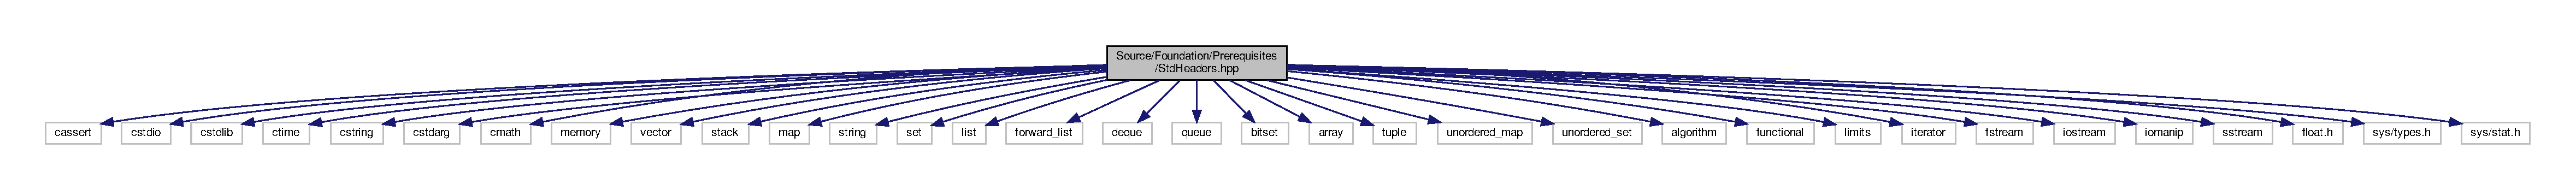
\includegraphics[width=350pt]{_std_headers_8hpp__incl}
\end{center}
\end{figure}
이 그래프는 이 파일을 직/간접적으로 include 하는 파일들을 보여줍니다.\+:\nopagebreak
\begin{figure}[H]
\begin{center}
\leavevmode
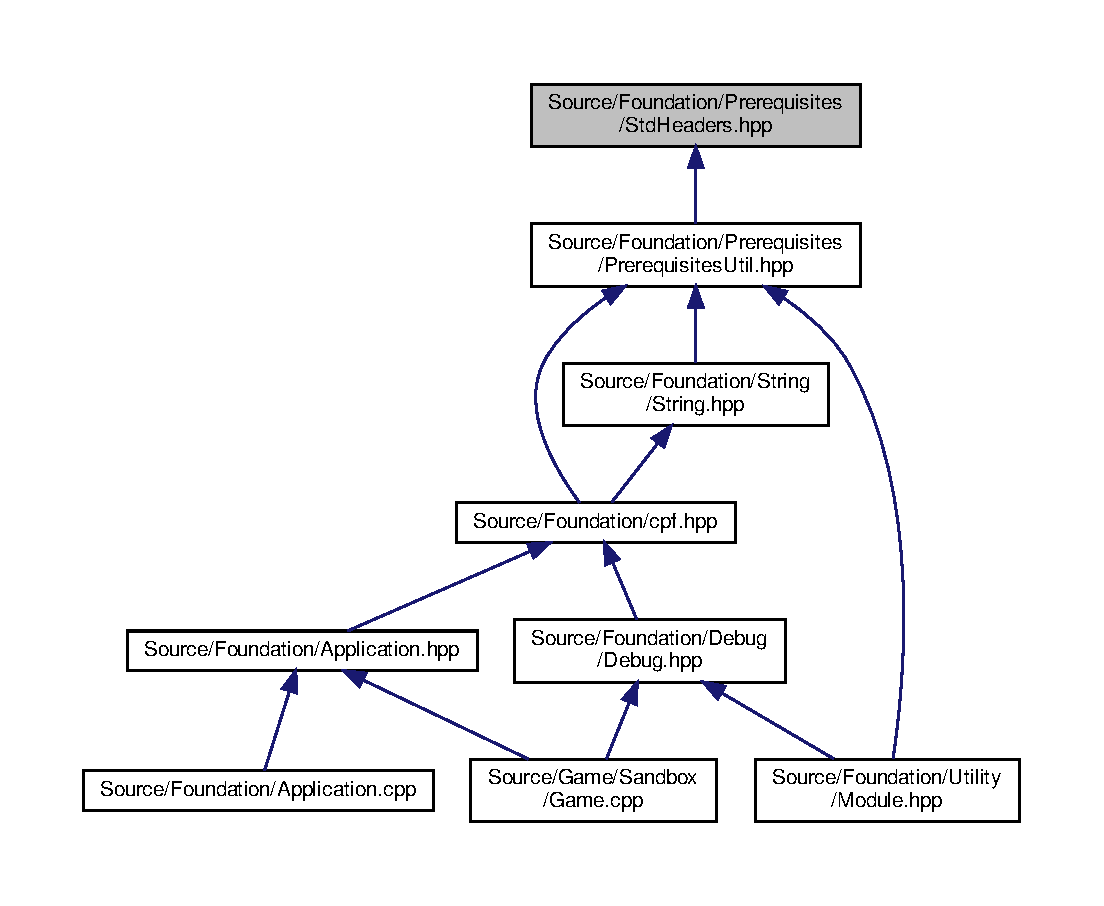
\includegraphics[width=350pt]{_std_headers_8hpp__dep__incl}
\end{center}
\end{figure}

\hypertarget{_string_8cpp}{}\section{Source/\+Foundation/\+String/\+String.cpp 파일 참조}
\label{_string_8cpp}\index{Source/\+Foundation/\+String/\+String.\+cpp@{Source/\+Foundation/\+String/\+String.\+cpp}}

\hypertarget{_string_8hpp}{}\section{Source/\+Foundation/\+String/\+String.hpp 파일 참조}
\label{_string_8hpp}\index{Source/\+Foundation/\+String/\+String.\+hpp@{Source/\+Foundation/\+String/\+String.\+hpp}}
{\ttfamily \#include $<$string$>$}\newline
{\ttfamily \#include \char`\"{}Prerequisites/\+Prerequisites\+Util.\+hpp\char`\"{}}\newline
String.\+hpp에 대한 include 의존 그래프\nopagebreak
\begin{figure}[H]
\begin{center}
\leavevmode
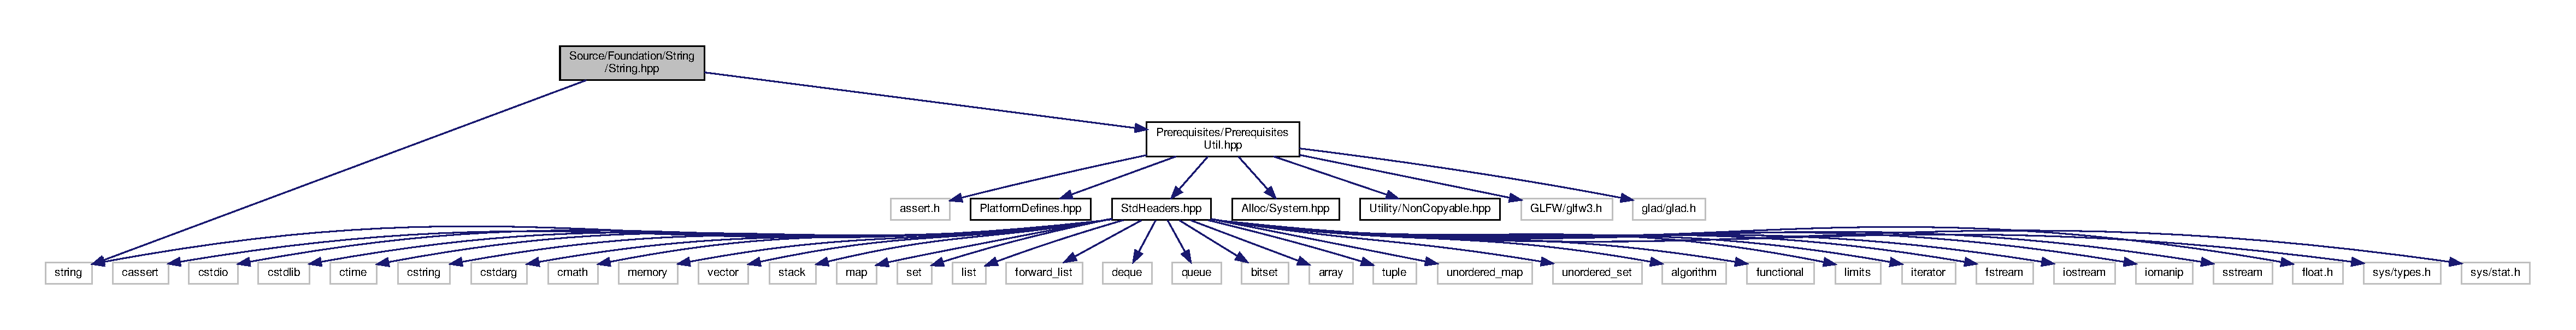
\includegraphics[width=350pt]{_string_8hpp__incl}
\end{center}
\end{figure}
이 그래프는 이 파일을 직/간접적으로 include 하는 파일들을 보여줍니다.\+:\nopagebreak
\begin{figure}[H]
\begin{center}
\leavevmode
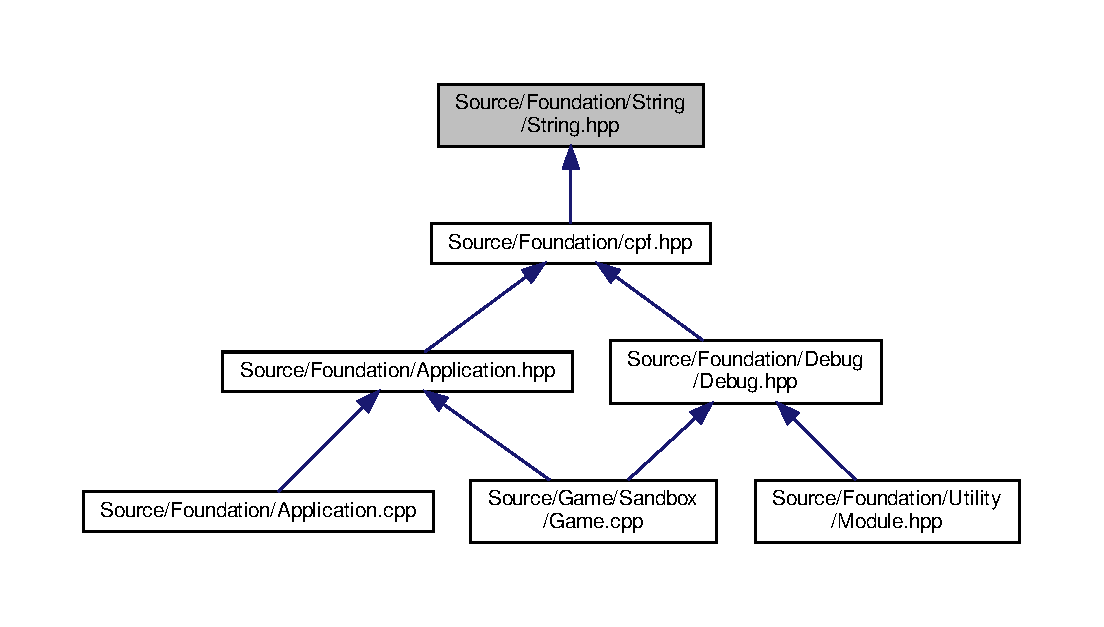
\includegraphics[width=350pt]{_string_8hpp__dep__incl}
\end{center}
\end{figure}
\subsection*{클래스}
\begin{DoxyCompactItemize}
\item 
class \hyperlink{classcpf_1_1_string_util}{cpf\+::\+String\+Util}
\end{DoxyCompactItemize}
\subsection*{네임스페이스}
\begin{DoxyCompactItemize}
\item 
 \hyperlink{namespacecpf}{cpf}
\end{DoxyCompactItemize}
\subsection*{타입정의}
\begin{DoxyCompactItemize}
\item 
{\footnotesize template$<$typename T $>$ }\\using \hyperlink{namespacecpf_ac91c8c57a370a5bef21ac23f876ad536}{cpf\+::\+Basic\+String} = std\+::basic\+\_\+string$<$ T, std\+::char\+\_\+traits$<$ T $>$ $>$
\item 
{\footnotesize template$<$typename T $>$ }\\using \hyperlink{namespacecpf_a1fe334b3d2422535a1cfe51785d98cb8}{cpf\+::\+Basic\+String\+Stream} = std\+::basic\+\_\+stringstream$<$ T, std\+::char\+\_\+traits$<$ T $>$ $>$
\item 
using \hyperlink{namespacecpf_a4dbd6992c3ed4440ce7ed8982ff7ffea}{cpf\+::\+String} = Basic\+String$<$ char $>$
\item 
using \hyperlink{namespacecpf_ad36115a5fb55fb1cc257eeab6aed2d7a}{cpf\+::\+W\+String} = Basic\+String$<$ wchar\+\_\+t $>$
\item 
using \hyperlink{namespacecpf_a32926a91098f8ea8d354b9f234b75acc}{cpf\+::\+U16\+String} = Basic\+String$<$ char16\+\_\+t $>$
\item 
using \hyperlink{namespacecpf_a71279c3a3d59ed723c48245204f8c0e5}{cpf\+::\+U32\+String} = Basic\+String$<$ char32\+\_\+t $>$
\item 
using \hyperlink{namespacecpf_a6e5583a51165e808f1a480563a2d98b2}{cpf\+::\+String\+Stream} = Basic\+String\+Stream$<$ char $>$
\item 
using \hyperlink{namespacecpf_a7e79dec7a6790331bee7ef1e85dafba6}{cpf\+::\+W\+String\+Stream} = Basic\+String\+Stream$<$ wchar\+\_\+t $>$
\item 
using \hyperlink{namespacecpf_a401e80bf9227c14c3f1f27121ba489d1}{cpf\+::\+U16\+String\+Stream} = Basic\+String\+Stream$<$ char16\+\_\+t $>$
\item 
using \hyperlink{namespacecpf_a7e95b195d831b69d8e661dd685128097}{cpf\+::\+U32\+String\+Stream} = Basic\+String\+Stream$<$ char32\+\_\+t $>$
\end{DoxyCompactItemize}

\hypertarget{_module_8hpp}{}\section{Source/\+Foundation/\+Utility/\+Module.hpp 파일 참조}
\label{_module_8hpp}\index{Source/\+Foundation/\+Utility/\+Module.\+hpp@{Source/\+Foundation/\+Utility/\+Module.\+hpp}}
{\ttfamily \#include \char`\"{}Prerequisites/\+Prerequisites\+Util.\+hpp\char`\"{}}\newline
{\ttfamily \#include \char`\"{}Debug/\+Debug.\+hpp\char`\"{}}\newline
Module.\+hpp에 대한 include 의존 그래프\nopagebreak
\begin{figure}[H]
\begin{center}
\leavevmode
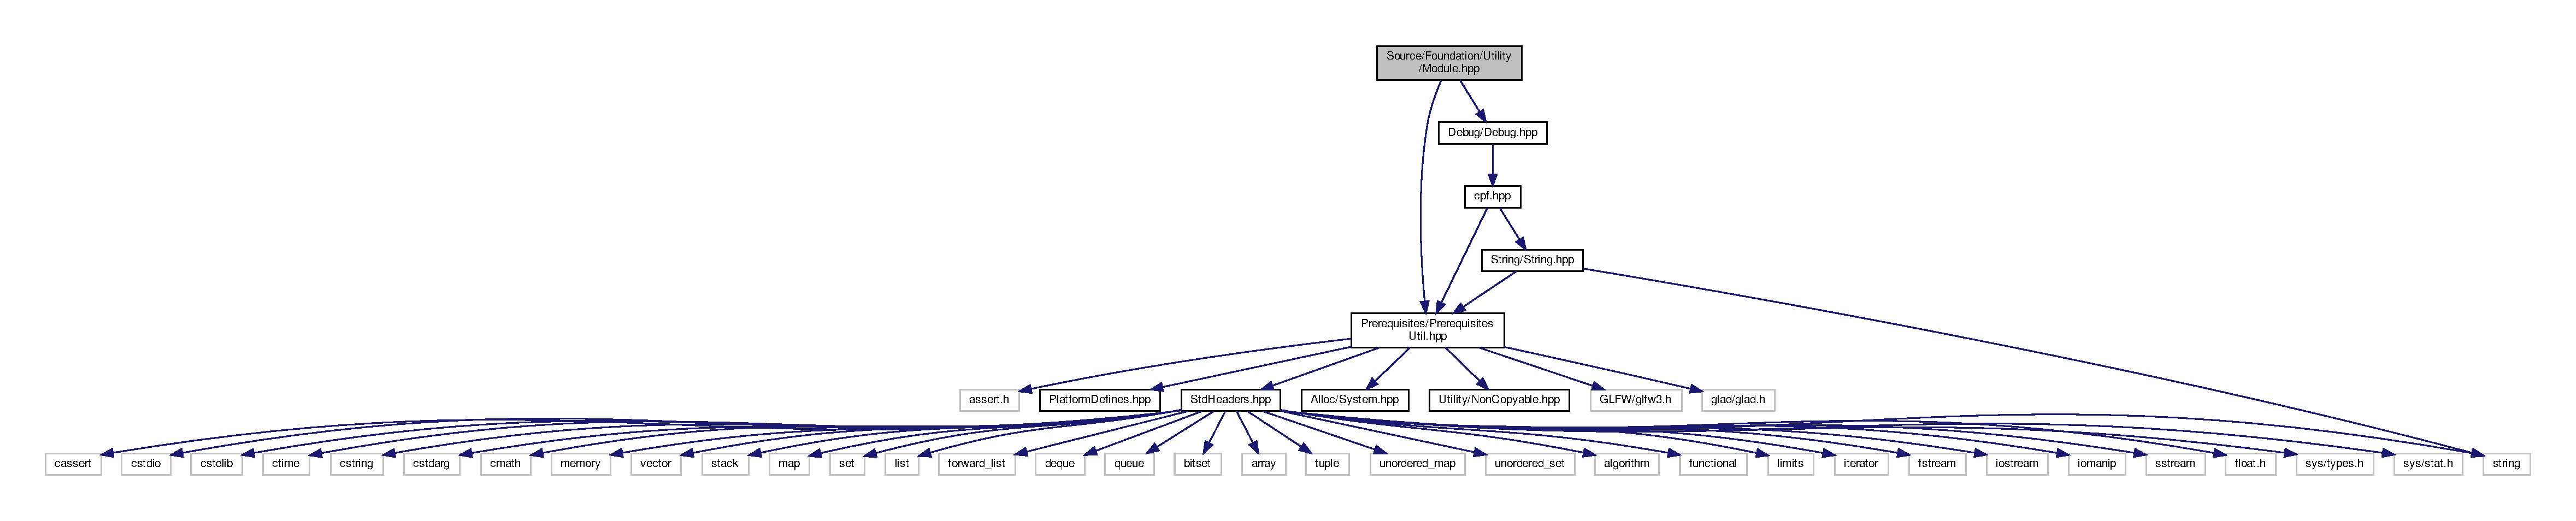
\includegraphics[width=350pt]{_module_8hpp__incl}
\end{center}
\end{figure}
\subsection*{클래스}
\begin{DoxyCompactItemize}
\item 
class \hyperlink{classcpf_1_1_t_module}{cpf\+::\+T\+Module$<$ T $>$}
\end{DoxyCompactItemize}
\subsection*{네임스페이스}
\begin{DoxyCompactItemize}
\item 
 \hyperlink{namespacecpf}{cpf}
\end{DoxyCompactItemize}
\subsection*{매크로}
\begin{DoxyCompactItemize}
\item 
\#define \hyperlink{_module_8hpp_abe137d157f9db724af4c9416d5d234de}{T\+M\+O\+D\+U\+L\+E\+\_\+\+I\+M\+P\+L\+E\+M\+E\+NT}(E\+X\+P\+O\+R\+T\+\_\+\+M\+A\+C\+RO,  C\+L\+A\+S\+S\+N\+A\+ME)
\end{DoxyCompactItemize}


\subsection{매크로 문서화}
\mbox{\Hypertarget{_module_8hpp_abe137d157f9db724af4c9416d5d234de}\label{_module_8hpp_abe137d157f9db724af4c9416d5d234de}} 
\index{Module.\+hpp@{Module.\+hpp}!T\+M\+O\+D\+U\+L\+E\+\_\+\+I\+M\+P\+L\+E\+M\+E\+NT@{T\+M\+O\+D\+U\+L\+E\+\_\+\+I\+M\+P\+L\+E\+M\+E\+NT}}
\index{T\+M\+O\+D\+U\+L\+E\+\_\+\+I\+M\+P\+L\+E\+M\+E\+NT@{T\+M\+O\+D\+U\+L\+E\+\_\+\+I\+M\+P\+L\+E\+M\+E\+NT}!Module.\+hpp@{Module.\+hpp}}
\subsubsection{\texorpdfstring{T\+M\+O\+D\+U\+L\+E\+\_\+\+I\+M\+P\+L\+E\+M\+E\+NT}{TMODULE\_IMPLEMENT}}
{\footnotesize\ttfamily \#define T\+M\+O\+D\+U\+L\+E\+\_\+\+I\+M\+P\+L\+E\+M\+E\+NT(\begin{DoxyParamCaption}\item[{}]{E\+X\+P\+O\+R\+T\+\_\+\+M\+A\+C\+RO,  }\item[{}]{C\+L\+A\+S\+S\+N\+A\+ME }\end{DoxyParamCaption})}



Module.\+hpp 파일의 9 번째 라인에서 정의되었습니다.


\hypertarget{_non_copyable_8hpp}{}\section{Source/\+Foundation/\+Utility/\+Non\+Copyable.hpp 파일 참조}
\label{_non_copyable_8hpp}\index{Source/\+Foundation/\+Utility/\+Non\+Copyable.\+hpp@{Source/\+Foundation/\+Utility/\+Non\+Copyable.\+hpp}}
이 그래프는 이 파일을 직/간접적으로 include 하는 파일들을 보여줍니다.\+:
\nopagebreak
\begin{figure}[H]
\begin{center}
\leavevmode
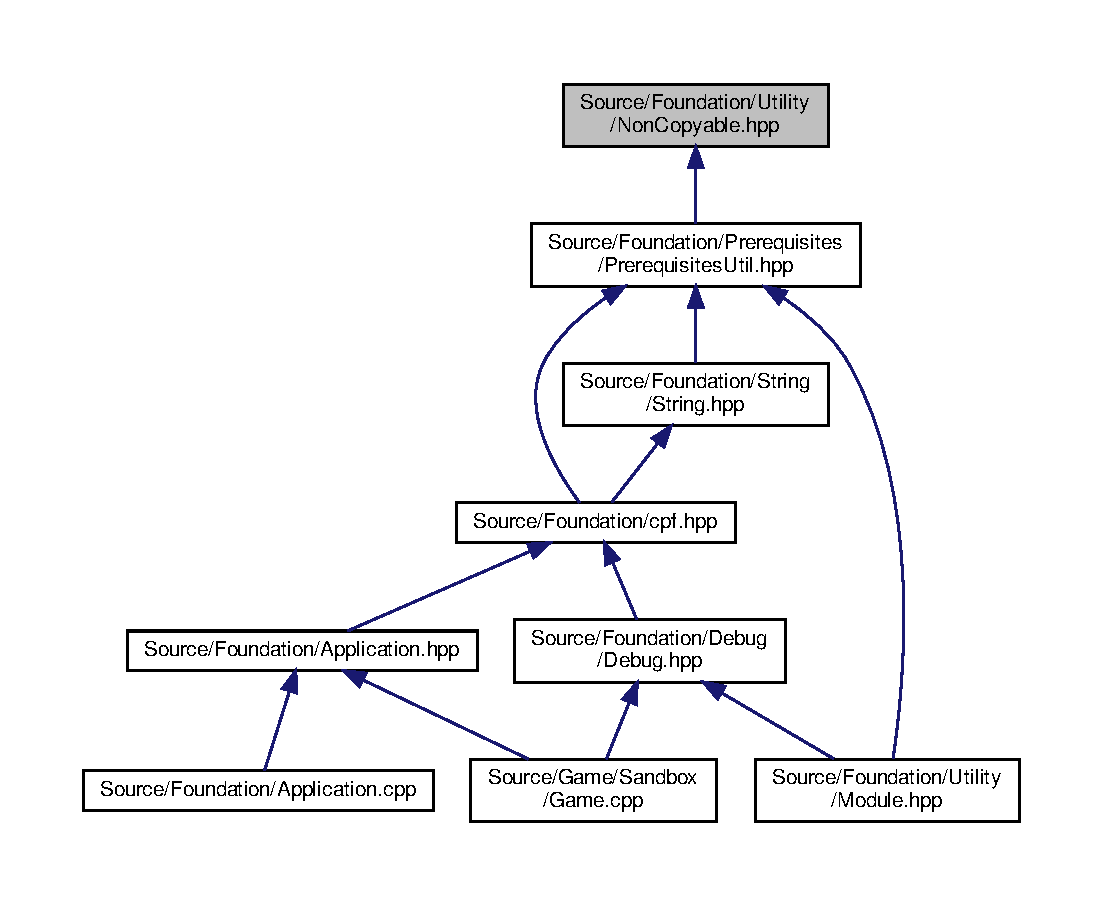
\includegraphics[width=350pt]{_non_copyable_8hpp__dep__incl}
\end{center}
\end{figure}
\subsection*{클래스}
\begin{DoxyCompactItemize}
\item 
class \hyperlink{classcpf_1_1_non_copyable}{cpf\+::\+Non\+Copyable}
\end{DoxyCompactItemize}
\subsection*{네임스페이스}
\begin{DoxyCompactItemize}
\item 
 \hyperlink{namespacecpf}{cpf}
\end{DoxyCompactItemize}

\hypertarget{_game_8cpp}{}\section{Source/\+Game/\+Sandbox/\+Game.cpp 파일 참조}
\label{_game_8cpp}\index{Source/\+Game/\+Sandbox/\+Game.\+cpp@{Source/\+Game/\+Sandbox/\+Game.\+cpp}}
{\ttfamily \#include \char`\"{}Application.\+hpp\char`\"{}}\newline
{\ttfamily \#include \char`\"{}Debug/\+Debug.\+hpp\char`\"{}}\newline
Game.\+cpp에 대한 include 의존 그래프\nopagebreak
\begin{figure}[H]
\begin{center}
\leavevmode
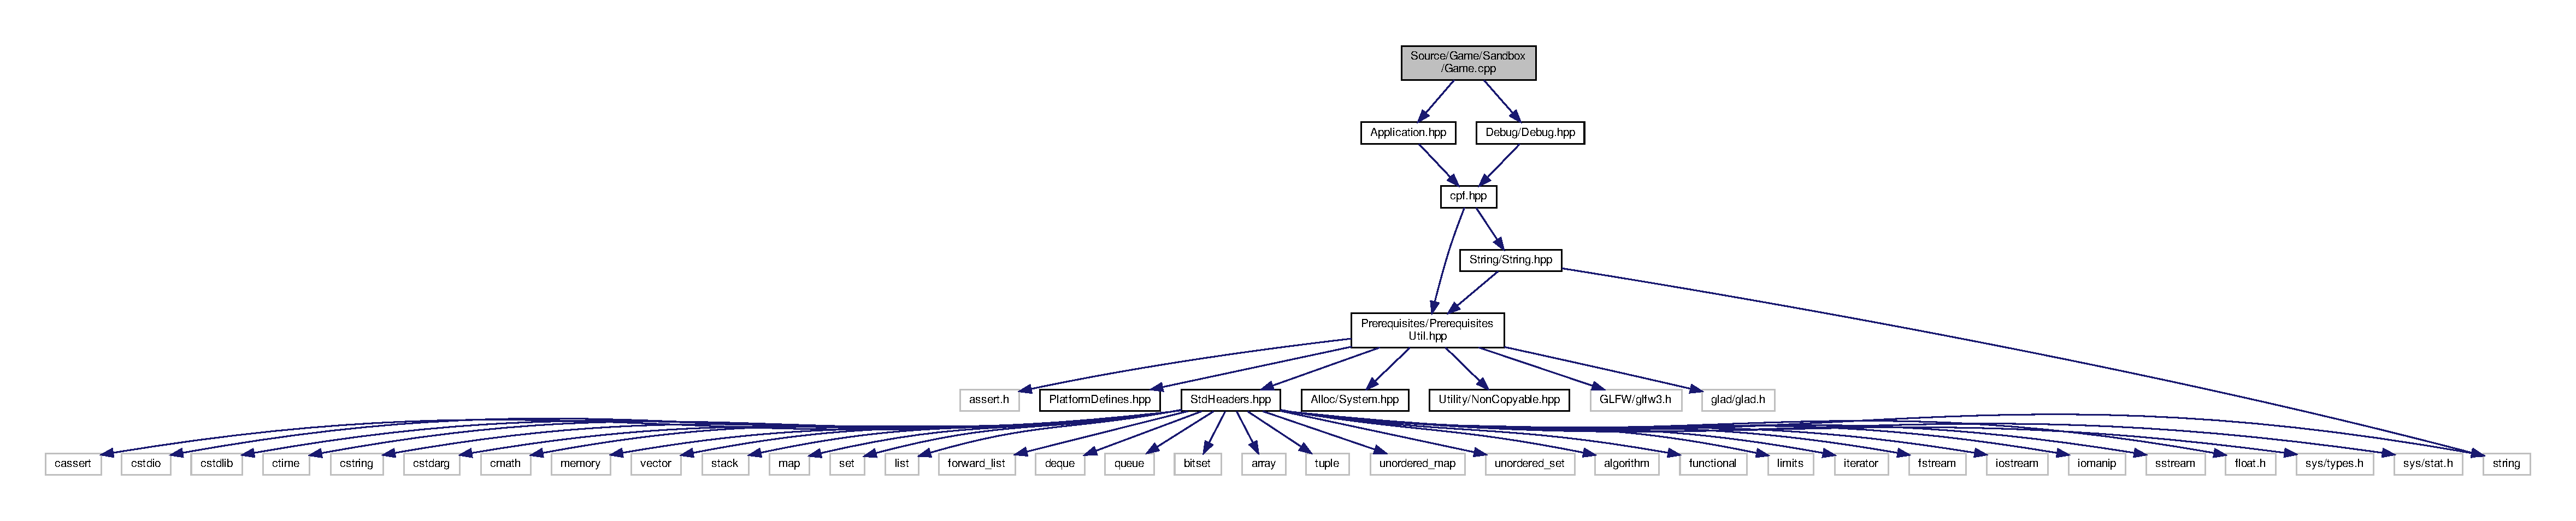
\includegraphics[width=350pt]{_game_8cpp__incl}
\end{center}
\end{figure}
\subsection*{함수}
\begin{DoxyCompactItemize}
\item 
int \hyperlink{_game_8cpp_ae66f6b31b5ad750f1fe042a706a4e3d4}{main} ()
\end{DoxyCompactItemize}


\subsection{함수 문서화}
\mbox{\Hypertarget{_game_8cpp_ae66f6b31b5ad750f1fe042a706a4e3d4}\label{_game_8cpp_ae66f6b31b5ad750f1fe042a706a4e3d4}} 
\index{Game.\+cpp@{Game.\+cpp}!main@{main}}
\index{main@{main}!Game.\+cpp@{Game.\+cpp}}
\subsubsection{\texorpdfstring{main()}{main()}}
{\footnotesize\ttfamily int main (\begin{DoxyParamCaption}{ }\end{DoxyParamCaption})}



Game.\+cpp 파일의 6 번째 라인에서 정의되었습니다.


\begin{DoxyCode}
6            \{
7     Debug::LogInfo(\textcolor{stringliteral}{"\{\}, \{\}"}, \textcolor{stringliteral}{"Hello"}, \textcolor{stringliteral}{"World"});
8     Debug::LogInfo(\textcolor{stringliteral}{"\{1\}, \{0\}"}, 1, \textcolor{stringliteral}{"World"});
9     Debug::LogWarning(\textcolor{stringliteral}{"\{\}, \{\}"}, \textcolor{stringliteral}{"This is"}, \textcolor{stringliteral}{"Warning!"});
10     Debug::LogError(\textcolor{stringliteral}{"\{\}, \{\}"}, \textcolor{stringliteral}{"Oh my GOD!"}, \textcolor{stringliteral}{"Error!"});
11     Debug::LogFatal(\textcolor{stringliteral}{"\{\}, \{\}, \{\}"}, \textcolor{stringliteral}{"Good norning"}, \textcolor{stringliteral}{"Good afternoon"}, \textcolor{stringliteral}{"Good evening"});
12 
13     \textcolor{keywordflow}{return} 0;
14 \}
\end{DoxyCode}

%--- End generated contents ---

% Index
\backmatter
\newpage
\phantomsection
\clearemptydoublepage
\addcontentsline{toc}{chapter}{색인}
\printindex

\end{document}
